% =============================================================
%  main.tex  --  Root-Dokument: ROS 2-Robotik-Handbuch
%  Compile:  latexmk -pdf main.tex
%            pdflatex main && bibtex main && pdflatex main && pdflatex main
% =============================================================

\documentclass[11pt,a4paper]{report}

% ---------- Preamble (packages, colors, styles, commands) ----------
% =============================================================
%  preamble.tex  --  Packages, styles, custom commands
%  Included by main.tex via % =============================================================
%  preamble.tex  --  Packages, styles, custom commands
%  Included by main.tex via % =============================================================
%  preamble.tex  --  Packages, styles, custom commands
%  Included by main.tex via \input{preamble}
% =============================================================

% ---------- Encoding & language ----------
\usepackage[utf8]{inputenc}
\usepackage[T1]{fontenc}
\usepackage[ngerman]{babel}
\usepackage{lmodern}

% ---------- Math ----------
\usepackage{amsmath,amssymb,bm}

% ---------- Layout ----------
\usepackage[a4paper,margin=2.3cm]{geometry}
\usepackage{parskip}
\usepackage{enumitem}
\setlist{nosep,leftmargin=1.4em}
\usepackage{booktabs}
\usepackage{tabularx}
\usepackage{longtable}
\usepackage{graphicx}
\usepackage{caption}
\captionsetup{font=small,labelfont=bf}

% ---------- Colors ----------
\usepackage{xcolor}
\definecolor{accent}{RGB}{20,90,160}
\definecolor{accent2}{RGB}{180,70,20}
\definecolor{codebg}{RGB}{245,246,248}
\definecolor{codekw}{RGB}{0,90,160}
\definecolor{codecom}{RGB}{100,120,100}
\definecolor{codestr}{RGB}{160,60,30}
\definecolor{rule}{RGB}{200,205,212}

% ---------- Headers ----------
\usepackage{fancyhdr}
\pagestyle{fancy}
\fancyhf{}
\renewcommand{\headrulewidth}{0.4pt}
\fancyhead[L]{\small\nouppercase{\leftmark}}
\fancyhead[R]{\small\thepage}
\fancypagestyle{plain}{%
  \fancyhf{}
  \fancyhead[R]{\small\thepage}
  \renewcommand{\headrulewidth}{0pt}%
}

% ---------- Code listings ----------
\usepackage{listings}
\lstdefinestyle{base}{
  backgroundcolor=\color{codebg},
  basicstyle=\ttfamily\footnotesize,
  keywordstyle=\color{codekw}\bfseries,
  commentstyle=\color{codecom}\itshape,
  stringstyle=\color{codestr},
  numbers=left, numberstyle=\tiny\color{gray}, numbersep=7pt,
  showstringspaces=false, breaklines=true, frame=single,
  rulecolor=\color{rule}, framesep=5pt, xleftmargin=14pt,
  tabsize=2, captionpos=b, aboveskip=8pt, belowskip=6pt,
}
\lstdefinestyle{py}{style=base,language=Python}
\lstdefinestyle{cpp}{style=base,language=C++}
\lstdefinestyle{bash}{style=base,language=bash,keywordstyle=\color{accent2}\bfseries}
\lstdefinestyle{xml}{style=base,language=XML,%
  morekeywords={link,joint,visual,collision,inertial,origin,axis,parent,child,%
    limit,mass,inertia,geometry,mesh,robot,transmission,actuator}}
\lstdefinestyle{yaml}{style=base,basicstyle=\ttfamily\footnotesize}

% ---------- Hyperref (load last among style packages) ----------
\usepackage[colorlinks=true,linkcolor=accent,urlcolor=accent2,citecolor=accent]{hyperref}

% ---------- TikZ ----------
\usepackage{tikz}
\usetikzlibrary{arrows.meta,positioning,shapes.geometric,fit,backgrounds,calc}
\usepackage{eurosym}
\tikzset{
  node/.style={draw,rounded corners=2pt,fill=accent!10,draw=accent,%
    font=\footnotesize\ttfamily,inner sep=4pt,align=center},
  topic/.style={draw,fill=accent2!8,draw=accent2,%
    font=\scriptsize\ttfamily,inner sep=3pt,align=center},
  flow/.style={-{Stealth[length=2mm]},thick,draw=gray!70},
}

% ---------- Custom coloured boxes ----------
\usepackage[most]{tcolorbox}
\newtcolorbox{infobox}[1][]{%
  colback=accent!5,colframe=accent!60,boxrule=0.6pt,arc=2pt,%
  left=6pt,right=6pt,top=4pt,bottom=4pt,fonttitle=\bfseries,#1}
\newtcolorbox{warnbox}[1][]{%
  colback=accent2!6,colframe=accent2!60,boxrule=0.6pt,arc=2pt,%
  left=6pt,right=6pt,top=4pt,bottom=4pt,fonttitle=\bfseries,#1}

% ---------- Inline code shorthand ----------
\newcommand{\code}[1]{\texttt{\small #1}}

% =============================================================

% ---------- Encoding & language ----------
\usepackage[utf8]{inputenc}
\usepackage[T1]{fontenc}
\usepackage[ngerman]{babel}
\usepackage{lmodern}

% ---------- Math ----------
\usepackage{amsmath,amssymb,bm}

% ---------- Layout ----------
\usepackage[a4paper,margin=2.3cm]{geometry}
\usepackage{parskip}
\usepackage{enumitem}
\setlist{nosep,leftmargin=1.4em}
\usepackage{booktabs}
\usepackage{tabularx}
\usepackage{longtable}
\usepackage{graphicx}
\usepackage{caption}
\captionsetup{font=small,labelfont=bf}

% ---------- Colors ----------
\usepackage{xcolor}
\definecolor{accent}{RGB}{20,90,160}
\definecolor{accent2}{RGB}{180,70,20}
\definecolor{codebg}{RGB}{245,246,248}
\definecolor{codekw}{RGB}{0,90,160}
\definecolor{codecom}{RGB}{100,120,100}
\definecolor{codestr}{RGB}{160,60,30}
\definecolor{rule}{RGB}{200,205,212}

% ---------- Headers ----------
\usepackage{fancyhdr}
\pagestyle{fancy}
\fancyhf{}
\renewcommand{\headrulewidth}{0.4pt}
\fancyhead[L]{\small\nouppercase{\leftmark}}
\fancyhead[R]{\small\thepage}
\fancypagestyle{plain}{%
  \fancyhf{}
  \fancyhead[R]{\small\thepage}
  \renewcommand{\headrulewidth}{0pt}%
}

% ---------- Code listings ----------
\usepackage{listings}
\lstdefinestyle{base}{
  backgroundcolor=\color{codebg},
  basicstyle=\ttfamily\footnotesize,
  keywordstyle=\color{codekw}\bfseries,
  commentstyle=\color{codecom}\itshape,
  stringstyle=\color{codestr},
  numbers=left, numberstyle=\tiny\color{gray}, numbersep=7pt,
  showstringspaces=false, breaklines=true, frame=single,
  rulecolor=\color{rule}, framesep=5pt, xleftmargin=14pt,
  tabsize=2, captionpos=b, aboveskip=8pt, belowskip=6pt,
}
\lstdefinestyle{py}{style=base,language=Python}
\lstdefinestyle{cpp}{style=base,language=C++}
\lstdefinestyle{bash}{style=base,language=bash,keywordstyle=\color{accent2}\bfseries}
\lstdefinestyle{xml}{style=base,language=XML,%
  morekeywords={link,joint,visual,collision,inertial,origin,axis,parent,child,%
    limit,mass,inertia,geometry,mesh,robot,transmission,actuator}}
\lstdefinestyle{yaml}{style=base,basicstyle=\ttfamily\footnotesize}

% ---------- Hyperref (load last among style packages) ----------
\usepackage[colorlinks=true,linkcolor=accent,urlcolor=accent2,citecolor=accent]{hyperref}

% ---------- TikZ ----------
\usepackage{tikz}
\usetikzlibrary{arrows.meta,positioning,shapes.geometric,fit,backgrounds,calc}
\usepackage{eurosym}
\tikzset{
  node/.style={draw,rounded corners=2pt,fill=accent!10,draw=accent,%
    font=\footnotesize\ttfamily,inner sep=4pt,align=center},
  topic/.style={draw,fill=accent2!8,draw=accent2,%
    font=\scriptsize\ttfamily,inner sep=3pt,align=center},
  flow/.style={-{Stealth[length=2mm]},thick,draw=gray!70},
}

% ---------- Custom coloured boxes ----------
\usepackage[most]{tcolorbox}
\newtcolorbox{infobox}[1][]{%
  colback=accent!5,colframe=accent!60,boxrule=0.6pt,arc=2pt,%
  left=6pt,right=6pt,top=4pt,bottom=4pt,fonttitle=\bfseries,#1}
\newtcolorbox{warnbox}[1][]{%
  colback=accent2!6,colframe=accent2!60,boxrule=0.6pt,arc=2pt,%
  left=6pt,right=6pt,top=4pt,bottom=4pt,fonttitle=\bfseries,#1}

% ---------- Inline code shorthand ----------
\newcommand{\code}[1]{\texttt{\small #1}}

% =============================================================

% ---------- Encoding & language ----------
\usepackage[utf8]{inputenc}
\usepackage[T1]{fontenc}
\usepackage[ngerman]{babel}
\usepackage{lmodern}

% ---------- Math ----------
\usepackage{amsmath,amssymb,bm}

% ---------- Layout ----------
\usepackage[a4paper,margin=2.3cm]{geometry}
\usepackage{parskip}
\usepackage{enumitem}
\setlist{nosep,leftmargin=1.4em}
\usepackage{booktabs}
\usepackage{tabularx}
\usepackage{longtable}
\usepackage{graphicx}
\usepackage{caption}
\captionsetup{font=small,labelfont=bf}

% ---------- Colors ----------
\usepackage{xcolor}
\definecolor{accent}{RGB}{20,90,160}
\definecolor{accent2}{RGB}{180,70,20}
\definecolor{codebg}{RGB}{245,246,248}
\definecolor{codekw}{RGB}{0,90,160}
\definecolor{codecom}{RGB}{100,120,100}
\definecolor{codestr}{RGB}{160,60,30}
\definecolor{rule}{RGB}{200,205,212}

% ---------- Headers ----------
\usepackage{fancyhdr}
\pagestyle{fancy}
\fancyhf{}
\renewcommand{\headrulewidth}{0.4pt}
\fancyhead[L]{\small\nouppercase{\leftmark}}
\fancyhead[R]{\small\thepage}
\fancypagestyle{plain}{%
  \fancyhf{}
  \fancyhead[R]{\small\thepage}
  \renewcommand{\headrulewidth}{0pt}%
}

% ---------- Code listings ----------
\usepackage{listings}
\lstdefinestyle{base}{
  backgroundcolor=\color{codebg},
  basicstyle=\ttfamily\footnotesize,
  keywordstyle=\color{codekw}\bfseries,
  commentstyle=\color{codecom}\itshape,
  stringstyle=\color{codestr},
  numbers=left, numberstyle=\tiny\color{gray}, numbersep=7pt,
  showstringspaces=false, breaklines=true, frame=single,
  rulecolor=\color{rule}, framesep=5pt, xleftmargin=14pt,
  tabsize=2, captionpos=b, aboveskip=8pt, belowskip=6pt,
}
\lstdefinestyle{py}{style=base,language=Python}
\lstdefinestyle{cpp}{style=base,language=C++}
\lstdefinestyle{bash}{style=base,language=bash,keywordstyle=\color{accent2}\bfseries}
\lstdefinestyle{xml}{style=base,language=XML,%
  morekeywords={link,joint,visual,collision,inertial,origin,axis,parent,child,%
    limit,mass,inertia,geometry,mesh,robot,transmission,actuator}}
\lstdefinestyle{yaml}{style=base,basicstyle=\ttfamily\footnotesize}

% ---------- Hyperref (load last among style packages) ----------
\usepackage[colorlinks=true,linkcolor=accent,urlcolor=accent2,citecolor=accent]{hyperref}

% ---------- TikZ ----------
\usepackage{tikz}
\usetikzlibrary{arrows.meta,positioning,shapes.geometric,fit,backgrounds,calc}
\usepackage{eurosym}
\tikzset{
  node/.style={draw,rounded corners=2pt,fill=accent!10,draw=accent,%
    font=\footnotesize\ttfamily,inner sep=4pt,align=center},
  topic/.style={draw,fill=accent2!8,draw=accent2,%
    font=\scriptsize\ttfamily,inner sep=3pt,align=center},
  flow/.style={-{Stealth[length=2mm]},thick,draw=gray!70},
}

% ---------- Custom coloured boxes ----------
\usepackage[most]{tcolorbox}
\newtcolorbox{infobox}[1][]{%
  colback=accent!5,colframe=accent!60,boxrule=0.6pt,arc=2pt,%
  left=6pt,right=6pt,top=4pt,bottom=4pt,fonttitle=\bfseries,#1}
\newtcolorbox{warnbox}[1][]{%
  colback=accent2!6,colframe=accent2!60,boxrule=0.6pt,arc=2pt,%
  left=6pt,right=6pt,top=4pt,bottom=4pt,fonttitle=\bfseries,#1}

% ---------- Inline code shorthand ----------
\newcommand{\code}[1]{\texttt{\small #1}}


% ---------- Graphics search path ----------
\graphicspath{{figures/}}

% ---------- Bibliography style ----------
\usepackage[backend=bibtex,style=numeric,sorting=none]{biblatex}
\addbibresource{back/bibliography.bib}

% =============================================================
\begin{document}

% ---- Front matter ----
% =============================================================
%  front/titlepage.tex  --  Custom title page
% =============================================================

\begin{titlepage}
  \centering
  \vspace*{2cm}

  {\Huge\bfseries ROS\,2-Robotik-Handbuch\par}
  \vspace{0.5cm}
  {\Large Theoretische Grundlagen, Hardware, Simulation und vier Projekte\par}
  \vspace{0.8cm}
  {\large
    Stepper-Robotik mit Zykloidgetriebe
    \,$\cdot$\, Stereokamera
    \,$\cdot$\, Kalman-Filter
    \,$\cdot$\, ROS\,2
  \par}

  \vspace{2.5cm}
  \rule{0.6\textwidth}{0.4pt}\\[0.4cm]

  {\large\itshape Arbeitsdokument\par}
  \vspace{0.4cm}
  {\normalsize
    Stand: Juni 2026\\[4pt]
    ROS\,2 Jazzy Jalisco \,/\, Gazebo Harmonic
  \par}

  \vfill
  \rule{0.6\textwidth}{0.4pt}
\end{titlepage}

\pagenumbering{roman}
\setcounter{page}{1}

% =============================================================
%  front/abstract.tex  --  Abstract / Kurzfassung
% =============================================================

\chapter*{Über dieses Dokument}
\addcontentsline{toc}{chapter}{Über dieses Dokument}

\begin{infobox}[title=Wie dieses Dokument zu lesen ist]
Das Handbuch ist in sechs Teile gegliedert.
\textbf{Teil~I} legt die Theorie fest (ROS\,2, Kalman/EKF, Odometrie, Stereosehen,
Kinematik, Dynamik, Trajektorien, Schrittmotoren, Zykloidgetriebe).
\textbf{Teil~II} behandelt die Hardware-Auswahl inklusive Strom-/Spannungsmessung
zur Drehmomentschätzung und PCB-Optimierung.
\textbf{Teil~III} ist die Schritt-für-Schritt-Installationsanleitung (VM, Linux,
ROS\,2).
\textbf{Teil~IV} erklärt die Simulation, den CAD-zu-URDF-Workflow und die
entscheidende Frage, wo sich Simulation und reale Implementierung trennen.
\textbf{Teil~V} arbeitet die vier Projekte mit Knoten-Architektur und
\code{rqt\_graph} durch.
\textbf{Teil~VI} ist die praktische Stereokamera-Integration mit Codebeispielen.
Den Abschluss bildet eine empfohlene Dokumentationsmethodik.
\end{infobox}


\clearpage
\tableofcontents
\clearpage

\pagenumbering{arabic}
\setcounter{page}{1}

% =============================================================
% TEIL I  --  Theoretische Grundlagen
%   (Maschinelles Lernen ist hierher gewandert: ch29)
% =============================================================
\part{Theoretische Grundlagen}

% =============================================================
%  ch01_ros2_konzepte.tex  --  ROS 2: Konzepte und Architektur
% =============================================================

\chapter{ROS\,2 -- Konzepte und Architektur}

\section{Warum ROS\,2 und nicht ROS\,1}
ROS\,2 ersetzt den zentralen \code{rosmaster} von ROS\,1 durch eine dezentrale
Discovery über \textbf{DDS} (Data Distribution Service), einen Industriestandard
aus Luft- und Raumfahrt. Daraus folgen die für deine Projekte relevanten
Eigenschaften: kein Single-Point-of-Failure, Multi-Maschinen-Betrieb über das
Netzwerk ohne Master, konfigurierbare Echtzeit-/Zuverlässigkeitsgarantien (QoS)
und ein einheitliches API in C++ (\code{rclcpp}) und Python (\code{rclpy}).
ROS\,1 (Noetic) ist seit Mai 2025 End-of-Life; alle Neuprojekte gehören auf
ROS\,2.

\section{Die fünf Kommunikationsprimitive}
Das gesamte Verhalten eines ROS\,2-Systems lässt sich auf fünf Bausteine
zurückführen. Sie zu verstehen ist die halbe Miete -- der Rest ist Anwendung.

\begin{description}[leftmargin=1.6em,style=nextline]
\item[Node (Knoten)] Eine Recheneinheit mit genau einer Verantwortung --
  z.\,B.\ \code{ball\_detector}, \code{trajectory\_controller}. Knoten
  kommunizieren ausschließlich über die vier folgenden Mechanismen, nie direkt.
\item[Topic (Thema)] Asynchroner Publish/Subscribe-Kanal, many-to-many. Ein
  Publisher sendet \emph{Nachrichten} (eines \code{.msg}-Typs), beliebig viele
  Subscriber empfangen sie. Geeignet für kontinuierliche Datenströme: Bilder,
  Gelenkzustände, Odometrie. \emph{Feuern und vergessen} -- der Sender weiß
  nicht, wer zuhört.
\item[Service (Dienst)] Synchroner Request/Response, one-to-one. Ein Client
  schickt eine Anfrage, ein Server antwortet genau einmal. Für kurze,
  abgeschlossene Aktionen: ``Schalte Controller um'', ``Gib aktuelle
  Kalibrierung zurück''. Blockierend.
\item[Action (Aktion)] Für lange, zielgerichtete Aufgaben mit
  Zwischen-Feedback und Abbruchmöglichkeit. Technisch aus Topics + Services
  zusammengesetzt: \emph{Goal} (Ziel senden), \emph{Feedback} (Fortschritt),
  \emph{Result} (Endergebnis). Der Paradefall für ``fahre diese Trajektorie
  ab'' -- du willst Fortschritt sehen und abbrechen können.
\item[Parameter] Pro Knoten gehaltene Konfigurationswerte (Gelenklimits,
  PID-Gains, Getriebeübersetzung), zur Laufzeit les- und setzbar, deklariert
  beim Knotenstart.
\end{description}

\begin{infobox}[title=Faustregel zur Wahl]
Kontinuierlicher Datenstrom $\rightarrow$ \textbf{Topic}.
Kurze Frage mit sofortiger Antwort $\rightarrow$ \textbf{Service}.
Langer Auftrag mit Fortschritt/Abbruch (Trajektorie, Navigation, Greifen)
$\rightarrow$ \textbf{Action}.
Statische Konfiguration $\rightarrow$ \textbf{Parameter}.
\end{infobox}

\section{QoS -- Quality of Service}
Weil DDS darunterliegt, hat jedes Topic eine QoS-Konfiguration. Die wichtigsten
Profile:
\begin{itemize}
\item \textbf{Reliability:} \code{RELIABLE} (jede Nachricht garantiert,
  Wiederübertragung) vs.\ \code{BEST\_EFFORT} (verlustbehaftet, aber
  latenzarm). Sensorbilder fahren oft \code{BEST\_EFFORT}, Steuerbefehle
  \code{RELIABLE}.
\item \textbf{Durability:} \code{TRANSIENT\_LOCAL} hält die letzte Nachricht für
  später startende Subscriber vor (typisch für \code{/map}, statische TF).
\item \textbf{History/Depth:} Puffergröße.
\end{itemize}
Eine häufige Fehlerquelle: Publisher und Subscriber mit \emph{inkompatiblen}
QoS-Profilen ``sehen'' sich nicht. Bei stummen Topics ist das der erste Verdacht.

\section{Workspace, Pakete, Build}
ROS\,2-Code lebt in einem \textbf{Workspace} (Verzeichnis mit \code{src/}).
Darin liegen \textbf{Pakete}. Gebaut wird mit \textbf{colcon}.
\begin{lstlisting}[style=bash,caption={Workspace anlegen und bauen}]
mkdir -p ~/ros2_ws/src && cd ~/ros2_ws
# ... Pakete nach src/ ...
rosdep install --from-paths src --ignore-src -y   # Abhaengigkeiten
colcon build --symlink-install                    # bauen
source install/setup.bash                         # Overlay aktivieren
\end{lstlisting}
Python-Pakete nutzen \code{ament\_python} (\code{setup.py}), C++-Pakete
\code{ament\_cmake} (\code{CMakeLists.txt}). Beide haben eine
\code{package.xml} mit Metadaten und Abhängigkeiten.

\section{TF2 -- der Transformationsbaum}
Jeder Roboter ist ein Baum von Koordinatensystemen (Frames):
\code{map} $\rightarrow$ \code{odom} $\rightarrow$ \code{base\_link}
$\rightarrow$ \code{camera\_link} $\rightarrow \dots$.
\textbf{TF2} verwaltet diese zeitgestempelten Transformationen, sodass du
jederzeit fragen kannst ``Wo ist der Ball im \code{base\_link}-Frame?'', obwohl
er in \code{camera\_link} gemessen wurde. Rotationen werden hier als
\textbf{Quaternionen} gespeichert (\code{geometry\_msgs/Quaternion}) -- genau aus
den Gründen, die wir besprochen haben: kein Gimbal Lock, kompakt, sauber
interpolierbar. Konventionen sind in REP-103 (Einheiten, rechtshändig, $x$
vorne, $z$ oben) und REP-105 (Frame-Namen) festgelegt.

\section{Wichtige CLI-Werkzeuge}
\begin{longtable}{@{}p{6.2cm}p{9cm}@{}}
\toprule
\textbf{Befehl} & \textbf{Zweck} \\
\midrule
\code{ros2 run <pkg> <node>}       & Einen Knoten starten \\
\code{ros2 launch <pkg> <file>}    & Mehrere Knoten + Konfiguration starten \\
\code{ros2 topic list / echo / hz} & Topics auflisten, Inhalt sehen, Rate messen \\
\code{ros2 node list / info}       & Knoten und ihre Schnittstellen \\
\code{ros2 service call}           & Dienst manuell aufrufen \\
\code{ros2 action send\_goal}      & Aktion manuell starten \\
\code{ros2 param get / set / dump} & Parameter lesen/schreiben/sichern \\
\code{rqt\_graph}                  & Knoten-Topic-Graph visualisieren \\
\code{rviz2}                       & 3D-Visualisierung (\emph{kein} Simulator!) \\
\code{ros2 bag record / play}      & Datenströme aufzeichnen/abspielen \\
\midrule
\end{longtable}

\begin{warnbox}[title=Häufige Begriffsverwechslung]
\textbf{RViz2} ist ein \emph{Visualisierer} (zeigt Daten an), \textbf{Gazebo}
ist ein \emph{Simulator} (erzeugt Daten per Physik). Du wirst beide gleichzeitig
nutzen: Gazebo simuliert, RViz2 zeigt an.
\end{warnbox}

% =============================================================
%  ch02_kalman_ekf.tex  --  Zustandsschätzung: Kalman-Filter und EKF
% =============================================================

\chapter{Zustandsschätzung: Kalman-Filter und EKF}

\section{Das Grundproblem}
Du willst eine verborgene Größe (Position und Geschwindigkeit des
Tischtennisballs, Pose des Roboters) aus verrauschten, unvollständigen
Messungen schätzen -- und das, während sich der Zustand zeitlich ändert. Der
Kalman-Filter ist der optimale lineare Schätzer für genau dieses Problem unter
gaußschem Rauschen. Er hält nicht nur einen Schätzwert $\hat{\bm{x}}$, sondern
auch dessen \textbf{Unsicherheit} als Kovarianzmatrix $\bm{P}$.

\section{Lineares Zustandsraummodell}
\begin{align}
\bm{x}_k &= \bm{F}\,\bm{x}_{k-1} + \bm{B}\,\bm{u}_k + \bm{w}_k,
  & \bm{w}_k &\sim \mathcal{N}(\bm{0},\bm{Q})
  \quad\text{(Prozessrauschen)}\\
\bm{z}_k &= \bm{H}\,\bm{x}_k + \bm{v}_k,
  & \bm{v}_k &\sim \mathcal{N}(\bm{0},\bm{R})
  \quad\text{(Messrauschen)}
\end{align}
$\bm{F}$ = Systemmatrix (wie entwickelt sich der Zustand),
$\bm{B}$ = Steuermatrix,
$\bm{H}$ = Messmatrix (was misst der Sensor vom Zustand),
$\bm{Q}/\bm{R}$ = Rausch-Kovarianzen (deine wichtigsten Tuning-Größen).

\section{Die zwei Phasen}
Der Filter alterniert zwischen \textbf{Prädiktion} (Modell rechnet voraus,
Unsicherheit wächst) und \textbf{Korrektur} (Messung zieht zurück, Unsicherheit
sinkt).

\begin{infobox}[title=Prädiktion (Zeitschritt)]
\vspace{-6pt}
\begin{align*}
\hat{\bm{x}}_k^- &= \bm{F}\,\hat{\bm{x}}_{k-1} + \bm{B}\,\bm{u}_k \\
\bm{P}_k^-       &= \bm{F}\,\bm{P}_{k-1}\,\bm{F}^\top + \bm{Q}
\end{align*}
\end{infobox}
\begin{infobox}[title=Korrektur (Messupdate)]
\vspace{-6pt}
\begin{align*}
\bm{K}_k      &= \bm{P}_k^-\,\bm{H}^\top
  \left(\bm{H}\,\bm{P}_k^-\,\bm{H}^\top + \bm{R}\right)^{-1}
  &&\text{(Kalman-Gain)}\\
\hat{\bm{x}}_k &= \hat{\bm{x}}_k^-
  + \bm{K}_k\left(\bm{z}_k - \bm{H}\,\hat{\bm{x}}_k^-\right)
  &&\text{(Innovation gewichtet)}\\
\bm{P}_k      &= (\bm{I} - \bm{K}_k\,\bm{H})\,\bm{P}_k^-
\end{align*}
\end{infobox}
Der Gain $\bm{K}$ ist die Gewichtung: Ist die Messung präzise ($\bm{R}$ klein),
vertraut der Filter ihr; ist das Modell präzise ($\bm{Q}$ klein), glättet er
stärker.

\section{Extended Kalman Filter (EKF)}
Sobald System oder Messung \textbf{nichtlinear} sind -- und das sind sie in der
Robotik fast immer (Rotationen, Projektilflug mit Luftwiderstand,
Kameraprojektion) --, ersetzt man die Matrizen durch nichtlineare Funktionen
$\bm{f}(\cdot)$ und $\bm{h}(\cdot)$ und linearisiert sie pro Schritt über die
\textbf{Jacobi-Matrizen}:
\begin{equation}
\bm{F}_k = \left.\frac{\partial \bm{f}}{\partial \bm{x}}\right|_{\hat{\bm{x}}_{k-1}},
\qquad
\bm{H}_k = \left.\frac{\partial \bm{h}}{\partial \bm{x}}\right|_{\hat{\bm{x}}_k^-}
\end{equation}
Prädiktion nutzt dann $\hat{\bm{x}}_k^- = \bm{f}(\hat{\bm{x}}_{k-1},\bm{u}_k)$,
die Kovarianz-Updates verwenden $\bm{F}_k, \bm{H}_k$.
Der \textbf{UKF} (Unscented) vermeidet die Jacobi-Matrizen, indem er
``Sigma-Punkte'' durch die Nichtlinearität propagiert -- genauer bei starker
Krümmung, aber rechenintensiver. Für Lageschätzung mit Quaternionen nimmt man
den \textbf{Error-State/Multiplicative EKF} (Fehlerzustand als kleiner 3D-Rotationsvektor
im Tangentialraum, multiplikativ aufs Quaternion angewandt).

\section{Anwendung Tischtennisball (konstante Beschleunigung)}
Zustand $\bm{x} = [x,y,z,\dot{x},\dot{y},\dot{z}]^\top$, Schwerkraft als
bekannte Steuerung. Mit Zeitschritt $\Delta t$:
\begin{equation}
\bm{F} = \begin{pmatrix} \bm{I}_3 & \Delta t\,\bm{I}_3 \\ \bm{0} & \bm{I}_3 \end{pmatrix},\quad
\bm{B}\bm{u} = \begin{pmatrix} \tfrac{1}{2}\Delta t^2\,\bm{g} \\ \Delta t\,\bm{g} \end{pmatrix},\quad
\bm{g}=\begin{pmatrix}0\\0\\-9.81\end{pmatrix},\quad
\bm{H} = \begin{pmatrix} \bm{I}_3 & \bm{0} \end{pmatrix}
\end{equation}
Die Stereokamera liefert nur die Position (daher $\bm{H}$ projiziert auf die
ersten drei Komponenten); der Filter schätzt die Geschwindigkeit mit und
extrapoliert per Prädiktion (ohne Messupdate) den Flug bis zur Schlagebene --
das ist die Vorhersage des Abschlagzeitpunkts. Luftwiderstand und Magnus-Effekt
(Spin) machen das Modell nichtlinear $\rightarrow$ EKF, falls nötig.

% =============================================================
%  ch03_odometrie.tex  --  Odometrie und Sensorfusion
% =============================================================

\chapter{Odometrie und Sensorfusion}

\textbf{Odometrie} schätzt die Eigenbewegung aus inkrementellen Sensordaten.
\begin{itemize}
\item \textbf{Radodometrie:} Aus Encoder-Ticks und
  Differentialantriebs-Kinematik die Pose integrieren. Einfach, aber driftet
  (Schlupf, Rundungsfehler akkumulieren).
\item \textbf{Visuelle Odometrie (VO):} Bewegung aus der Verfolgung von
  Bildmerkmalen über aufeinanderfolgende Frames schätzen. Mit Stereokamera
  bekommst du den Maßstab gratis (Tiefe ist bekannt).
\item \textbf{Visual-Inertial Odometry (VIO):} VO + IMU per EKF fusioniert --
  robuster, glatter.
\end{itemize}
In ROS\,2 ist \textbf{\code{robot\_localization}} das Standardpaket: ein
\code{ekf\_node}/\code{ukf\_node} fusioniert mehrere Quellen (Rad-Odom + IMU +
visuelle Odom) zu einer konsistenten \code{odom}$\rightarrow$\code{base\_link}-Transformation.
Drift wird später durch SLAM/Loop-Closure korrigiert
(\code{map}$\rightarrow$\code{odom}).

% =============================================================
%  ch04_stereosehen.tex  --  Stereosehen und Merkmalserkennung
% =============================================================

\chapter{Stereosehen und Merkmalserkennung}
\label{ch:stereosehen}

\section{Lochkameramodell und Tiefe aus Disparität}
Eine kalibrierte Kamera bildet einen 3D-Punkt über die Intrinsik-Matrix $\bm{K}$
ab:
\begin{equation}
\bm{K} = \begin{pmatrix} f_x & 0 & c_x \\ 0 & f_y & c_y \\ 0 & 0 & 1 \end{pmatrix}
\end{equation}
Bei zwei horizontal um die \textbf{Basislinie} $b$ versetzten Kameras erscheint
ein Punkt im linken und rechten Bild an leicht verschiedener Spalte; die
Differenz ist die \textbf{Disparität} $d$. Die Tiefe folgt direkt:
\begin{equation}
\boxed{\,Z = \dfrac{f\cdot b}{d}\,}
\end{equation}
Große Basislinie $\rightarrow$ bessere Tiefenauflösung in der Ferne, aber
kleinerer überlappender Sichtbereich in der Nähe. Die Disparität wird auf
\emph{rektifizierten} Bildern berechnet (beide Bildebenen koplanar,
Epipolarlinien horizontal), typisch mit \code{StereoBM} (schnell) oder
\code{StereoSGBM} (genauer) aus OpenCV.

\section{Kalibrierung}
Beide Kameras müssen kalibriert werden (Intrinsik + Verzerrung) und zueinander
(Extrinsik: $\bm{R},\bm{t}$ zwischen den Linsen). Standard ist ein
Schachbrettmuster \cite{opencv_calib} und das ROS\,2-Paket
\code{camera\_calibration} aus dem
\code{image\_pipeline}. Ergebnis sind \code{.yaml}-Dateien, die der Treiber
lädt. \textbf{Ohne saubere Kalibrierung ist jede Tiefenmessung wertlos} -- das
ist der erste reale Stolperstein gegenüber der Simulation, wo die ``Kamera''
perfekt kalibriert ist. Schon kleine Kalibrierfehler skalieren systematisch in
die Objektgenauigkeit hinein \cite{kahmen2020stereocalib}; die praktische
Durchführung samt detektiertem Schachbrettmuster ist in
Kapitel~\ref{ch:kalibrierung} ausgeführt.

\section{Merkmalserkennung ohne eigenes KI-Training}
Es gibt ausgereifte \emph{klassische} Detektoren, die ohne Trainingsdaten und
ohne neuronale Netze auskommen. Sie finden markante, wiedererkennbare
Bildpunkte (Ecken, Blobs) und beschreiben deren lokale Umgebung:
\begin{longtable}{@{}p{2.4cm}p{4.5cm}p{8cm}@{}}
\toprule
\textbf{Detektor} & \textbf{Eigenschaft} & \textbf{Einsatz} \\
\midrule
\textbf{ORB}   & schnell, binär, lizenzfrei    & Echtzeit-Matching, VO, Standardwahl für Hobby \\
\textbf{SIFT}  & skalierungs-/rotationsinvariant, robust & genaues Matching, CAD-Posenschätzung \\
\textbf{AKAZE} & gute Balance                  & Alternative zu SIFT/ORB \\
\textbf{BRISK} & binär, schnell                & ressourcenarme Plattformen \\
\bottomrule
\end{longtable}
\noindent Alle sind in OpenCV enthalten (\code{cv2.ORB\_create()} usw.) und über
\code{cv\_bridge} in ROS\,2 nutzbar. Das Matching erfolgt mit \code{BFMatcher}
(Brute Force) oder \code{FLANN}, gefolgt von Ausreißerfilterung
(Lowe-Ratio-Test, RANSAC). Eine quantitative Gegenüberstellung von Genauigkeit
und Geschwindigkeit dieser Detektoren findet sich in
Kapitel~\ref{ch:merkmalserkennung} \cite{tareen2018comparative}. Für \textbf{Bewegungserkennung} (Projekt~3) brauchst
du nicht einmal Merkmale: Hintergrundsubtraktion
(\code{cv2.createBackgroundSubtractorMOG2}) oder optischer Fluss
(\code{calcOpticalFlowFarneback}) reichen.

\section{Posenschätzung -- 6D-Lage eines Bauteils}
Für Projekt~4 (CAD-Matching) gibt es zwei Hauptwege:
\begin{enumerate}
\item \textbf{2D-3D über PnP:} Merkmale im Kamerabild gegen bekannte 3D-Punkte
  des CAD-Modells matchen, dann \code{cv2.solvePnPRansac()} liefert Rotation +
  Translation des Bauteils relativ zur Kamera.
\item \textbf{3D-3D über ICP:} Aus der Stereokamera eine Punktwolke erzeugen und
  per \textbf{Iterative Closest Point} an die aus dem CAD-Modell gesampelte
  Punktwolke anpassen (z.\,B.\ mit Open3D). Liefert die volle 6D-Pose, robust
  bei guter Initialschätzung.
\end{enumerate}
Das Ergebnis (Rotation als Quaternion + Translation) wird in TF veröffentlicht
und vom Greifplaner (MoveIt\,2) konsumiert.

% =============================================================
%  ch04a_posenschaetzung.tex  --  6-DoF-Posenschätzung mit gelernten
%  Surface Embeddings (theoretische Grundlagen für Projekt 4)
% =============================================================

\chapter{6-DoF-Posenschätzung mit gelernten Surface Embeddings}

Dieses Kapitel vertieft die theoretischen Grundlagen hinter Projekt~4. Es baut
direkt auf dem Stereosehen (Kapitel zuvor) auf: Dort wurde die 6D-Pose über
klassische Merkmale (\code{PnP}, \code{ICP}) bestimmt; hier wird der moderne,
lernbasierte Weg über \textbf{dichte Surface Embeddings} (in der Linie von
\textbf{SurfEmb} \cite{haugaard2022surfemb}) entwickelt, der bei
texturarmen, glänzenden oder symmetrischen Industrieteilen robuster ist.

\section{Das Problem: sechs Freiheitsgrade}
\textbf{6-DoF-Posenschätzung} bestimmt \emph{Position und Orientierung} eines
bekannten Bauteils -- drei Translations- und drei Rotationsfreiheitsgrade.
\textbf{Warum überhaupt?} Ein Werkstück liegt selten zweimal gleich (Schüttgut
in Kisten, verschobene Vorrichtung, Förderband). Der Roboter muss das Teil
\emph{sehen}, bevor er greift. Gesucht ist die starre Transformation, die das
bekannte CAD-Modell in das Kamera-/Roboterkoordinatensystem überführt:
\begin{equation}
\boxed{\;\bm{p}_{\text{cam}} = \bm{R}\,\bm{p}_{\text{model}} + \bm{t}\;}
\qquad \bm{R}\in SO(3),\;\; \bm{t}\in\mathbb{R}^3
\end{equation}
Die rücktransformierte (``ausgerichtete'') Punktwolke ist nur die visuelle
Bestätigung -- das eigentliche Ergebnis ist $(\bm{R},\bm{t})$.

\section{Rotationsrepräsentationen}
Die Translation ist trivial ($\mathbb{R}^3$); die Rotation ist der heikle Teil,
weil $SO(3)$ gekrümmt ist. Gängige Darstellungen mit ihren Fallstricken:
\begin{longtable}{@{}p{3.6cm}p{10.6cm}@{}}
\toprule
\textbf{Darstellung} & \textbf{Eigenschaft / Fallstrick} \\
\midrule
Rotationsmatrix ($3{\times}3$) & 9 Zahlen, 6 Nebenbedingungen (orthonormal); redundant aber stabil \\
Euler-Winkel              & nur 3 Zahlen, aber \textbf{Gimbal Lock} (Freiheitsgrad-Verlust) \\
Quaternion                & 4 Zahlen, singularitätsfrei, aber \textbf{Double Cover} ($\bm{q}$ und $-\bm{q}$ = gleiche Drehung) \\
Kontinuierliche 6D-Form   & beste Wahl für die \textbf{NN-Regression} -- stetig, keine Sprünge \cite{zhou2019continuity} \\
\bottomrule
\end{longtable}
\noindent Für neuronale Netze ist die Stetigkeit entscheidend: Euler und
Quaternion haben Unstetigkeiten, an denen das Netz schlecht lernt. Die
6D-Darstellung (zwei Spaltenvektoren $\rightarrow$ Gram-Schmidt $\rightarrow$
$\bm{R}$) ist überall stetig.

\section{Warum gelernte Embeddings statt Regression}
Zwei naive Wege scheitern in der Industrie:
\begin{itemize}
\item \textbf{Handgefertigte Deskriptoren} (\code{FPFH} \cite{rusu2009fpfh},
  \code{SIFT}) versagen bei texturlosen, glänzenden, symmetrischen Teilen und
  unter Verdeckung -- genau die typischen Fälle in der Fertigung.
\item \textbf{Direkte Pose-Regression} (Netz $\rightarrow$ ein $(\bm{R},\bm{t})$)
  nimmt \emph{eine} Antwort an (unimodal) und \textbf{bricht bei Symmetrie}: ein
  symmetrisches Teil hat mehrere korrekte Posen, der Mittelwert ist falsch.
\end{itemize}
\textbf{Gelernte dichte Surface Embeddings} lösen beides: Ein Netz bildet jeden
Oberflächenpunkt in einen Merkmalsraum ab; gemessene Punkte werden über die
\emph{Nähe im Merkmalsraum} den Punkten des bekannten CAD-Modells zugeordnet.
Statt einer Punktschätzung lernt das Modell eine \textbf{Verteilung} über
Korrespondenzen -- Symmetrie wird implizit behandelt (mehrere Oberflächenpunkte
teilen sich dann schlicht ein Embedding) \cite{haugaard2022surfemb}.

\section{Kontrastives Lernen der Embeddings}
Trainiert werden die Embeddings mit einem \textbf{kontrastiven Verlust}: wahre
Pixel-$\leftrightarrow$-Punkt-Paare werden im Merkmalsraum zusammengezogen, alle
anderen Paare auseinandergedrückt. Die \emph{Positiv}-Paare sind die unter
bekannter Render-Pose bekannten Korrespondenzen, die \emph{Negativ}-Paare andere
gesampelte Oberflächenpunkte. In InfoNCE-Form für ein Query-Embedding $\bm{q}$
mit positivem Schlüssel $\bm{k}^+$:
\begin{equation}
\mathcal{L} = -\log
\frac{\exp\!\big(\mathrm{sim}(\bm{q},\bm{k}^+)/\tau\big)}
     {\sum_{j}\exp\!\big(\mathrm{sim}(\bm{q},\bm{k}_j)/\tau\big)}
\end{equation}
mit Kosinus-Ähnlichkeit $\mathrm{sim}(\cdot)$ und \textbf{Temperatur} $\tau$
(Tuning-Größe). \textbf{Der Clou:} die Labels sind quasi gratis -- man rendert
das CAD-Modell in bekannten Posen, womit Ground-Truth-Pose \emph{und}
Korrespondenzen automatisch vorliegen; keine manuellen Symmetrie-Labels nötig.

\section{Das Two-Tower-Modell (Query--Key)}
Die Architektur besteht aus zwei getrennten Türmen, die erst im gemeinsamen
Embedding-Raum zusammentreffen:
\begin{itemize}
\item \textbf{Query-Tower} -- \emph{Eingang:} Bildausschnitt (2D-Pixel, RGB/RGB-D);
  \emph{Ausgang:} Embedding pro Pixel; \emph{Architektur:} großes
  CNN-Encoder-Decoder-Netz (U-Net / ResNet).
\item \textbf{Key-Tower} -- \emph{Eingang:} eine 3D-Oberflächenkoordinate
  $(x,y,z)$ vom CAD; \emph{Ausgang:} Embedding dieses Punktes im selben Raum;
  \emph{Architektur:} kleines MLP (wenige Schichten reichen, da der Eingang
  simpel ist -- die \textbf{Asymmetrie} der Türme ist gewollt).
\end{itemize}
Beide werden \emph{gemeinsam} mit dem kontrastiven Verlust trainiert, sodass
zusammengehörige Pixel- und Punkt-Embeddings nahe beieinander landen. Ein Turm
spricht ``2D-Bild'', der andere ``3D-Oberfläche''; der gemeinsame Raum ist die
gemeinsame Sprache.

\begin{center}
\begin{tikzpicture}[node distance=6mm,every node/.style={font=\scriptsize}]
\node[node] (img) {Bildausschnitt\\2D-Pixel (RGB/RGB-D)};
\node[node,below=of img] (cnn) {CNN Encoder-Decoder\\U-Net / ResNet (groß)};
\node[node,below=of cnn] (pe) {Embedding pro Pixel};
\node[node,fill=accent2!12,draw=accent2,right=42mm of img] (pt) {3D-Oberflächenpunkt\\$(x,y,z)$ vom CAD};
\node[node,fill=accent2!12,draw=accent2,below=of pt] (mlp) {kleines MLP\\wenige Schichten};
\node[node,fill=accent2!12,draw=accent2,below=of mlp] (ke) {Embedding pro Punkt};
\node[node,fill=accent!18,below=12mm of $(pe)!0.5!(ke)$] (sh)
  {Gemeinsamer Embedding-Raum\\\itshape gemeinsam via kontrastivem Verlust trainiert};
\node[node,below=8mm of sh] (out)
  {Nächsten-Nachbarn-Matching\\dichte 2D-3D-Korrespondenzen $\rightarrow$ \code{PnP}+\code{RANSAC} $\rightarrow$ $(\bm{R},\bm{t})$};
\draw[flow] (img)--(cnn); \draw[flow] (cnn)--(pe);
\draw[flow] (pt)--(mlp);  \draw[flow] (mlp)--(ke);
\draw[flow] (pe)--(sh);   \draw[flow] (ke)--(sh);
\draw[flow] (sh)--(out);
\node[font=\scriptsize\bfseries,accent] at ($(cnn)+(0,1.0)$) {Query-Tower};
\node[font=\scriptsize\bfseries,accent2] at ($(mlp)+(0,1.0)$) {Key-Tower};
\end{tikzpicture}
\captionof{figure}{Two-Tower-Modell: die Türme bleiben getrennt bis zum
gemeinsamen Embedding-Raum -- genau diese Trennung \emph{ist} die Architektur.
Bei der Inferenz wird jedes Pixel-Embedding seinem nächsten
Oberflächenpunkt-Embedding zugeordnet.}
\end{center}

\section{Von Korrespondenzen zur Pose: PnP + RANSAC}
Aus den dichten 2D-3D-Korrespondenzen wird die Pose über \textbf{Perspective-n-Point}
(\code{PnP}) gelöst -- die $(\bm{R},\bm{t})$, die die 3D-Modellpunkte $\bm{P}_i$
auf die beobachteten Pixel $\bm{u}_i$ projiziert:
\begin{equation}
(\bm{R},\bm{t}) = \arg\min_{\bm{R},\bm{t}}
\sum_i \big\lVert \bm{u}_i - \pi\!\big(\bm{K}(\bm{R}\bm{P}_i + \bm{t})\big)\big\rVert^2
\end{equation}
mit Projektion $\pi(\cdot)$ und Intrinsik $\bm{K}$. \textbf{RANSAC} umhüllt das
Ganze und verwirft Ausreißer-Korrespondenzen (zieht zufällige minimale Mengen,
zählt Inlier, behält das beste Modell). Bei reinen 3D-3D-Daten tritt an die
Stelle der Reprojektion die euklidische Punktdistanz.

\section{Registrierung: grob und fein}
Eine \emph{einstufige} Registrierung ist unzuverlässig; Standard sind
\textbf{zwei Stufen}:
\begin{enumerate}
\item \textbf{Grob (global):} liefert die ``richtige Größenordnung'' aus
  Merkmalen -- Deskriptoren auf Quelle und Modell matchen, grobes
  $(\bm{R},\bm{t})$ lösen (z.\,B.\ \code{SAC-IA} + \code{FPFH}). Braucht
  \emph{keine} gute Startschätzung, ist aber nur näherungsweise.
\item \textbf{Fein = ICP} (\emph{Iterative Closest Point}
  \cite{besl1992icp}): zu jedem Quellpunkt den nächsten Zielpunkt suchen, die
  Gesamtdistanz minimieren, wiederholen bis zur Konvergenz:
  \begin{equation}
  E(\bm{R},\bm{t}) = \sum_i \big\lVert \bm{R}\,\bm{p}_i + \bm{t} - \bm{q}_{c(i)}\big\rVert^2,
  \qquad c(i)=\text{nächster Nachbar}
  \end{equation}
  Genau, aber nur \textbf{lokal}.
\end{enumerate}
\textbf{ICP-Schwächen:} (1) \emph{lokale Minima} -- es läuft bergab und bleibt
stecken; (2) \emph{initialisierungsabhängig} -- es funktioniert nur bei nahem
Start (daher läuft die Grobstufe zuerst). \textbf{Go-ICP}
\cite{yang2016goicp} garantiert das globale Optimum, indem es ganz $SE(3)$ (alle
starren Transformationen) per \emph{Branch-and-Bound} durchsucht: Raum
aufteilen, Fehler je Region beschränken, Regionen verwerfen, die nicht gewinnen
können -- langsamer, aber global optimal.

\section{Punktwolken-Netze: PointNet und PointNet++}
Verarbeitet man die Punktwolke direkt mit einem Netz, ist die zentrale
Schwierigkeit: eine Punktwolke ist eine \textbf{ungeordnete Menge} -- der Ausgang
darf nicht von der Reihenfolge abhängen (\textbf{Permutationsinvarianz}).
\begin{itemize}
\item \textbf{PointNet} \cite{qi2017pointnet}: dasselbe geteilte MLP auf jeden
  Punkt, dann \textbf{Max-Pooling} (symmetrisch = reihenfolgeunabhängig). Erfasst
  die \emph{globale} Form, verpasst aber lokale Details.
\item \textbf{PointNet++} \cite{qi2017pointnetpp}: wendet PointNet
  \emph{lokal} in Stufen an -- Zentren samplen (Farthest-Point-Sampling),
  Nachbarschaften gruppieren (Multi-Scale-Radien), lokale Merkmale extrahieren,
  auf größerer Skala wiederholen. Baut lokal + global hierarchisch auf, ähnlich
  einem CNN.
\end{itemize}

\section{Stereo, Tiefe und Skalierung}
\textbf{Warum Stereo?} Eine Mono-Kamera hat \emph{Skalenmehrdeutigkeit}
(klein-nah $\approx$ groß-fern). Stereo liefert Tiefe und löst die Skala -- über
Disparität, Basislinie und Brennweite (Triangulation, vgl.\ Stereo-Kapitel).
Zwei Wege in die Pipeline:
\begin{enumerate}[label=(\alph*)]
\item Tiefe als \textbf{Zusatzkanal} = RGB-D-Eingang, oder
\item Tiefe + Intrinsik \textbf{rückprojizieren} $\rightarrow$ Punktwolke
  $\rightarrow$ 3D-3D-Registrierung.
\end{enumerate}
\textbf{Vorverarbeitung} (vor dem Netz, ja): Kalibrierung (Intrinsik +
Extrinsik) und Rektifizierung, Tiefen-Entrauschung, Umgang mit ungültiger Tiefe
(glänzendes Metall liefert schlechte Tiefenwerte). \textbf{Auszahlung:} die
Tiefe gibt \emph{metrische} Skala -- $(\bm{R},\bm{t})$ in echten Millimetern, mit
denen der Roboter handeln kann.

\section{Zeitliche Konsistenz: Kalman-Pose-Tracking}
Eine bildweise geschätzte Pose ist verrauscht/zittrig. Ein \textbf{Kalman-Filter}
ergänzt \emph{zeitliche Konsistenz} (vgl.\ Kapitel zu Kalman/EKF): der
\emph{Zustand} ist die Pose (ggf.\ plus Geschwindigkeit), die \emph{Messung} ist
die bildweise Netz-Pose. Prädiktion der nächsten Pose $\rightarrow$ Korrektur mit
der neuen Schätzung. Das \textbf{glättet Jitter, verwirft Ausreißer-Frames und
überbrückt kurze Verdeckung / ausgefallene Detektionen} -- aus Einzelschuss wird
\emph{Tracking}, relevant für bewegtes Förderband oder armmontierte Kamera. Da
Rotationen nichtlinear sind, nutzt man EKF/UKF oder filtert auf einer geeigneten
Rotationsdarstellung.

\section{Sim-to-Real und Trainingsdaten}
Da die Labels durch Rendern des CAD-Modells praktisch gratis entstehen, wird
synthetisch trainiert -- aber es klafft ein \textbf{Sim-to-Real-Gap}
(synthetisch $\rightarrow$ real: Rauschen, Beleuchtung, Reflektanz). Gegenmittel:
\textbf{Domain Randomization}, physikalisch-basiertes Rendering (PBR, z.\,B.\ via
Isaac Sim, vgl.\ Kapitel zu Simulationswerkzeugen) und ein kleiner realer
Feintuning-Datensatz.

\section{Benchmarking und Metriken}
\begin{longtable}{@{}p{3.8cm}p{10.4cm}@{}}
\toprule
\textbf{Größe} & \textbf{Bedeutung} \\
\midrule
\textbf{ADD / ADD-S}     & mittlerer Punktabstand Modell$\leftrightarrow$Schätzung; ADD-S nutzt nächsten Punkt (für \emph{symmetrische} Teile) \\
Rotations-/Translationsfehler & geodätisch (Rotation) bzw.\ euklidisch (Translation), dazu RMSE \\
\textbf{BOP}-Metriken    & VSD, MSSD, MSPD $\rightarrow$ Average Recall \cite{hodan2018bop} \\
Industrie-KPIs           & Taktzeit/Latenz, Pick-Erfolgsrate, Falsch-Positiv-Rate \\
Datensätze               & BOP-Suite, speziell \textbf{T-LESS} und \textbf{ITODD} (texturlos/industriell) \\
\bottomrule
\end{longtable}

\begin{infobox}[title=Kernaussage in einem Satz]
6-DoF-Posenschätzung über gelernte Surface Embeddings ersetzt fragile
handgefertigte Deskriptoren durch ein \emph{Zwei-Turm-Netz}, das Pixel und
CAD-Oberflächenpunkte in einen gemeinsamen Merkmalsraum abbildet; das dichte
Korrespondenz-Matching liefert über \code{PnP}+\code{RANSAC} (optional
ICP-verfeinert) die starre Transformation $(\bm{R},\bm{t})$ -- robust auch bei
texturlosen, glänzenden und symmetrischen Teilen.
\end{infobox}

% =============================================================
%  ch05_kinematik.tex  --  Kinematik, Dynamik und Trajektorien
% =============================================================

\chapter{Kinematik, Dynamik und Trajektorien}

\section{Vorwärtskinematik}
Aus den Gelenkwinkeln $\bm{q}$ die Endeffektor-Pose berechnen. Klassisch über
die Kette homogener $4\times4$-Transformationen (Denavit-Hartenberg-Parameter).
Der Rotationsblock jeder Transformation ist eine $3\times3$-Matrix; intern
äquivalent zur Quaternion-Darstellung.

\section{Inverse Kinematik}
Aus der gewünschten Pose die Gelenkwinkel finden. Numerisch über die
\textbf{Jacobi-Matrix} $\bm{J}$, die Gelenkgeschwindigkeiten auf
Endeffektorgeschwindigkeiten abbildet ($\dot{\bm{x}} = \bm{J}\dot{\bm{q}}$).
Iterativ:
\begin{equation}
\Delta\bm{q} = \bm{J}^{\dagger}\,\bm{e},
\qquad
\bm{e} = \begin{pmatrix}\bm{e}_{\text{pos}} \\ \bm{e}_{\text{ori}}\end{pmatrix}
\end{equation}
mit Pseudo-Inverser $\bm{J}^\dagger$ (oder Damped-Least-Squares nahe
Singularitäten). Der \textbf{Orientierungsfehler} $\bm{e}_{\text{ori}}$ wird als
Vektorteil des Fehlerquaternions $q_{\text{soll}}\otimes q_{\text{ist}}^{-1}$
gebildet -- Euler-Differenzen sind hier wegen Gimbal Lock unbrauchbar. In
ROS\,2 löst \textbf{MoveIt\,2} (mit KDL/TracIK) das für dich.

\section{Dynamik}
Das Bewegungsgesetz eines Roboterarms:
\begin{equation}
\bm{M}(\bm{q})\ddot{\bm{q}} + \bm{C}(\bm{q},\dot{\bm{q}})\dot{\bm{q}}
+ \bm{g}(\bm{q}) = \bm{\tau}
\end{equation}
$\bm{M}$ = Massenmatrix, $\bm{C}$ = Coriolis/Zentrifugal,
$\bm{g}$ = Gravitation, $\bm{\tau}$ = Gelenkmomente. Für die Simulation ist
entscheidend, dass du jedem Link in der URDF korrekte \textbf{Masse und
Trägheitstensoren} gibst -- sonst rechnet die Physik-Engine Unsinn.

\section{Trajektorienplanung}
\begin{itemize}
\item \textbf{Gelenkraum:} Kubische/quintische Polynome oder ein
  \textbf{trapezförmiges Geschwindigkeitsprofil} (beschleunigen -- konstant --
  abbremsen) erzeugen ruckarme, ableitungsstetige Verläufe.
\item \textbf{Kartesischer Raum:} Position linear interpolieren, Orientierung
  per \textbf{SLERP} (gleichmäßige Winkelgeschwindigkeit). Für glatte
  Mehrpunktbahnen \textbf{SQUAD}.
\end{itemize}
In ROS\,2 transportiert \code{trajectory\_msgs/JointTrajectory} eine Bahn
(Punkte mit Position/Geschwindigkeit/Zeit), und der
\code{joint\_trajectory\_controller} fährt sie ab.

% =============================================================
%  ch05a_regelungstechnik.tex  --  Regelungstechnik für Roboter:
%  Feedback, Vorsteuerung, Kaskade, Arbeitsraum, Feedback-Entkopplung,
%  Beobachter und Störgrößenkompensation
% =============================================================

\chapter{Regelungstechnik der Robotergrundlagen}
\label{ch:regelung}

Die Dynamik aus Kapitel~\ref{ch:kinematik} sagt, \emph{welches} Gelenkmoment
$\bm{\tau}$ eine gewünschte Bewegung erzeugt. Die Regelung beantwortet die
schwierigere Frage: Wie hält der Roboter die Sollbahn \textbf{trotz}
Modellfehlern, Reibung, Nutzlastwechseln und Stößen? Dieses Kapitel ordnet die
gängigen Regelungsarchitekturen ein -- mit dem Fokus, \textbf{wann} man welche
einsetzen \emph{muss} und worin der Unterschied zu den Alternativen liegt.

Grundlage ist überall das Bewegungsgesetz aus dem Kinematik-Kapitel:
\begin{equation}\label{eq:dyn}
\bm{M}(\bm{q})\ddot{\bm{q}} + \bm{C}(\bm{q},\dot{\bm{q}})\dot{\bm{q}}
+ \bm{g}(\bm{q}) = \bm{\tau} + \bm{\tau}_{\text{stör}}
\end{equation}
mit Massenmatrix $\bm{M}$, Coriolis/Zentrifugal-Term $\bm{C}$, Gravitation
$\bm{g}$ und einer Störung $\bm{\tau}_{\text{stör}}$ (Reibung, Kontaktkräfte,
unmodellierte Last). Der Bahnfehler ist $\bm{e} = \bm{q}_{\text{soll}} - \bm{q}$.

\section{Feedback: die Grundlage}
Feedback (Rückführung) misst den Fehler $\bm{e}$ und stellt ihm ein
korrigierendes Moment entgegen. Der Klassiker im Gelenkraum ist ein
\textbf{PD-Regler mit Gravitationskompensation}:
\begin{equation}
\bm{\tau} = \bm{K}_p\,\bm{e} + \bm{K}_d\,\dot{\bm{e}} + \bm{g}(\bm{q})
\end{equation}
\begin{infobox}[title=Wann einsetzen]
Immer -- Feedback ist das Fundament jeder Roboterregelung. Es ist die einzige
Komponente, die \emph{unbekannte} Störungen und Modellfehler nachträglich
ausbügelt. Ein reiner PD/PID im Gelenkraum genügt bei langsamen Bewegungen,
hoher Getriebeuntersetzung (entkoppelt die Gelenke quasi voneinander) und
moderaten Genauigkeitsanforderungen -- etwa beim Anfahren von Wegpunkten.
\end{infobox}
\textbf{Unterschied zu den anderen:} Feedback reagiert \emph{erst nach} dem
Auftreten des Fehlers -- es ist reaktiv und damit zwangsläufig
„hinterher``. Hohe $\bm{K}_p$ verkürzen die Reaktion, fachen aber Rauschen und
Schwingungen an. Alles Folgende (Vorsteuerung, Entkopplung, Beobachter) dient
dazu, dem Feedback weniger Arbeit zu hinterlassen.

\section{Vorsteuerung (Feedforward)}
Die Vorsteuerung rechnet aus der \emph{bekannten} Sollbahn das nötige Moment
\textbf{vorab} aus und schaltet es additiv zum Feedback. Mit dem Modell
\eqref{eq:dyn} ergibt sich die ideale \textbf{dynamische Vorsteuerung}:
\begin{equation}\label{eq:ff}
\bm{\tau} = \underbrace{\bm{M}(\bm{q})\ddot{\bm{q}}_{\text{soll}}
+ \bm{C}(\bm{q},\dot{\bm{q}})\dot{\bm{q}}_{\text{soll}} + \bm{g}(\bm{q})}
_{\text{Vorsteuerung (Modell)}}
+ \underbrace{\bm{K}_p\,\bm{e} + \bm{K}_d\,\dot{\bm{e}}}_{\text{Feedback}}
\end{equation}
Das ist eine \textbf{Zwei-Freiheitsgrade-Struktur}: Die Vorsteuerung bestimmt
das Führungsverhalten (Bahnfolge), das Feedback nur noch das Störverhalten
(Restfehler). Beide lassen sich getrennt auslegen.
\begin{infobox}[title=Wann einsetzen]
Sobald die Bahn \emph{im Voraus bekannt} ist und schnell/präzise gefolgt werden
soll -- Schweißnähte, Pick-and-Place mit kurzen Taktzeiten, der Schlagarm des
Tischtennisroboters. Die Vorsteuerung eliminiert den \emph{systematischen}
Schleppfehler, ohne die Feedback-Verstärkung hochziehen zu müssen.
\end{infobox}
\textbf{Unterschied zum Feedback:} Vorsteuerung ist \emph{vorausschauend} und
kennt keinen Messfehler -- sie kann daher nicht instabil werden, aber auch keine
unvorhergesehene Störung ausgleichen. Sie ist nur so gut wie das Modell. Darum
nie allein, sondern stets \emph{kombiniert} mit Feedback.

\section{Kaskadenregelung}
Statt einer einzigen Schleife schachtelt die Kaskade mehrere ineinander -- jede
mit eigener, messbarer Zwischengröße. Beim Servoantrieb sind das drei Ebenen:
\begin{center}
\begin{tikzpicture}[node distance=7mm]
\node[node] (pos) {Positions-\\regler};
\node[node,right=of pos] (vel) {Geschwindigkeits-\\regler};
\node[node,right=of vel] (cur) {Strom-/Momenten-\\regler};
\node[node,right=of cur,fill=accent!18] (mot) {Motor +\\Gelenk};
\draw[flow] (pos)--(vel) node[midway,above,font=\scriptsize]{$\dot q_{\text{soll}}$};
\draw[flow] (vel)--(cur) node[midway,above,font=\scriptsize]{$i_{\text{soll}}$};
\draw[flow] (cur)--(mot) node[midway,above,font=\scriptsize]{$u$};
\draw[flow] (mot.south) -- ++(0,-6mm) -| (vel.south)
  node[near start,below,font=\scriptsize]{$\dot q$ (Encoder)};
\draw[flow] (mot.south) -- ++(0,-11mm) -| (pos.south)
  node[near start,below,font=\scriptsize]{$q$ (Encoder)};
\end{tikzpicture}
\end{center}
Die \textbf{innere} Schleife (Strom) ist am schnellsten getaktet
($\sim$\,kHz--10\,kHz), die \textbf{äußere} (Position) am langsamsten. Faustregel:
jede innere Schleife mindestens 3--5$\times$ schneller als die nächstäußere.
\begin{infobox}[title=Wann einsetzen]
Praktisch in jedem industriellen Antrieb -- Servoverstärker und FOC-Treiber sind
intern bereits kaskadiert. Sinnvoll, sobald eine schnell messbare Zwischengröße
(Strom, Drehzahl) existiert und die Stellgröße begrenzt werden muss.
\end{infobox}
\textbf{Unterschied zu den anderen:} Die Kaskade ist eine \emph{strukturelle}
Anordnung mehrerer Feedback-Schleifen, kein eigenständiges Regelgesetz. Ihr
Vorteil: Störungen, die in einer inneren Schleife angreifen (z.\,B.
Versorgungsspannungs\-schwankungen), werden dort sofort abgefangen, bevor sie die
äußere erreichen; außerdem lässt sich jede Ebene einzeln in Betrieb nehmen und
sättigen (Anti-Windup, Strombegrenzung). Quer\-kopplungen zwischen den Gelenken
behandelt sie aber nicht -- dafür braucht es Entkopplung (s.\,u.).

\section{Feedback-Entkopplung (Computed Torque)}
Bei schnellen Bewegungen sind die Gelenke über $\bm{M}$ und $\bm{C}$ stark
\emph{gekoppelt}: ein bewegtes Gelenk übt Reaktionsmomente auf die anderen aus.
Die Feedback-Entkopplung (auch \textbf{inverse Dynamik}- oder
\textbf{Computed-Torque}-Regelung) hebt das per exakter Modellrechnung auf. Man
setzt eine Hilfsgröße $\bm{a}$ an und invertiert die Dynamik:
\begin{equation}\label{eq:ctc}
\bm{\tau} = \bm{M}(\bm{q})\,\bm{a}
+ \bm{C}(\bm{q},\dot{\bm{q}})\dot{\bm{q}} + \bm{g}(\bm{q}),
\qquad
\bm{a} = \ddot{\bm{q}}_{\text{soll}} + \bm{K}_d\,\dot{\bm{e}} + \bm{K}_p\,\bm{e}
\end{equation}
Eingesetzt in \eqref{eq:dyn} (ohne Störung) bleibt das exakt \textbf{lineare,
entkoppelte} Fehlersystem
\begin{equation}
\ddot{\bm{e}} + \bm{K}_d\,\dot{\bm{e}} + \bm{K}_p\,\bm{e} = \bm{0},
\end{equation}
also für \emph{jedes} Gelenk ein unabhängiges, frei platzierbares
PD-Verhalten -- unabhängig von Stellung und Geschwindigkeit.
\begin{infobox}[title=Wann einsetzen]
Schnelle, dynamische Bewegungen mit leichter Struktur und geringer
Getriebeunter\-setzung, bei denen die Kopplung spürbar wird -- Leichtbauarme,
Direktantriebe, der hochbeschleunigte Schlagarm. Voraussetzung: ein hinreichend
genaues Dynamikmodell und Momenten-/Strom\-regelbare Antriebe.
\end{infobox}
\textbf{Unterschied zur Vorsteuerung:} Beide nutzen das Modell. Die Vorsteuerung
\eqref{eq:ff} wertet es entlang der \emph{Soll}-Größen aus (Steuerung, offene
Wirkung); die Feedback-Entkopplung \eqref{eq:ctc} wertet $\bm{M},\bm{C}$ entlang
der \emph{Ist}-Größen aus und linearisiert die Strecke \emph{innerhalb} der
geschlossenen Schleife. Dadurch ist das resultierende Fehlerverhalten
arbeitspunktunabhängig konstant -- der Preis ist die Modellauswertung in
Echtzeit und die Empfindlichkeit gegen Modellfehler.

\section{Regelung im Arbeitsraum (Operational Space Control)}
Bisher wurde im Gelenkraum geregelt; die Aufgabe ist aber meist im
\textbf{kartesischen Raum} definiert (Pose des Endeffektors $\bm{x}$). Statt erst
per inverser Kinematik nach $\bm{q}_{\text{soll}}$ umzurechnen, formuliert man
Regler und Dynamik direkt in $\bm{x}$ -- über die Jacobi-Matrix $\bm{J}$ mit
$\dot{\bm{x}} = \bm{J}\dot{\bm{q}}$. Das entkoppelte Gesetz im Arbeitsraum lautet
\begin{equation}
\bm{\tau} = \bm{J}^\top\!\Big[\bm{\Lambda}(\bm{q})\,\bm{a}_x
+ \bm{\mu}(\bm{q},\dot{\bm{q}}) + \bm{p}(\bm{q})\Big],
\qquad
\bm{a}_x = \ddot{\bm{x}}_{\text{soll}}
+ \bm{K}_d\,\dot{\bm{e}}_x + \bm{K}_p\,\bm{e}_x
\end{equation}
mit der Arbeitsraum-Massenmatrix $\bm{\Lambda} = (\bm{J}\bm{M}^{-1}\bm{J}^\top)^{-1}$.
Der Fehler $\bm{e}_x$ wird direkt im kartesischen Raum gebildet (Position als
Differenz, Orientierung als Vektorteil des Fehlerquaternions, vgl.
Kapitel~\ref{ch:kinematik}).
\begin{infobox}[title=Wann einsetzen]
Wenn die \emph{Aufgabe} im kartesischen Raum lebt: Kraft-/Impedanz\-regelung beim
Kontakt (Polieren, Stecken, Montage), Bahnverfolgung am Werkstück,
nullraumoptimierte redundante Arme. Auch dann, wenn die inverse Kinematik nahe
Singularitäten unzuverlässig wird.
\end{infobox}
\textbf{Unterschied zur Gelenkraumregelung:} Identische Mathematik, anderer Raum.
Im Arbeitsraum legst du Steifigkeit und Dämpfung \emph{richtungsabhängig} fest
(z.\,B.\ nachgiebig in Stoßrichtung, steif quer dazu) -- ideal für Kontakt\-aufgaben.
Nachteil: $\bm{J}$ wird nahe Singularitäten schlecht konditioniert, und der
Nullraum redundanter Roboter muss separat behandelt werden.

\section{Zustandsbeobachter}
Computed-Torque und Vorsteuerung brauchen $\dot{\bm{q}}$ (oft auch
Beschleunigungen oder die Störung) -- gemessen wird aber meist nur die Position
$\bm{q}$. Numerisches Differenzieren verstärkt Rauschen. Der
\textbf{Zustandsbeobachter} schätzt die nicht gemessenen Zustände aus Modell und
Eingang, korrigiert über den Messfehler:
\begin{equation}
\dot{\hat{\bm{x}}} = \bm{f}(\hat{\bm{x}},\bm{u})
+ \bm{L}\,(\bm{y} - \hat{\bm{y}})
\end{equation}
Die Beobachterverstärkung $\bm{L}$ legt fest, wie schnell die Schätzung dem
wahren Zustand folgt (Luenberger für lineare, EKF für nichtlineare Systeme --
siehe Kapitel~\ref{ch:kalman}).
\begin{infobox}[title=Wann einsetzen]
Wenn Zustände für das Regelgesetz gebraucht werden, die kein Sensor direkt
liefert: Gelenkgeschwindigkeit aus reinem Positionsencoder, Verspannung in einem
elastischen Gelenk, oder -- besonders wichtig -- die \emph{Störung} selbst (s.\,u.).
\end{infobox}
\textbf{Unterschied zum Kalman-Filter:} Der Beobachter ist das deterministische
Konzept; der Kalman-Filter ist der Beobachter, dessen $\bm{L}$ statistisch
optimal aus den Rausch-Kovarianzen bestimmt wird. Funktional dasselbe Bauteil im
Regelkreis.

\section{Störgrößenkompensation}
Reibung, unbekannte Nutzlast und Kontaktkräfte stecken in
$\bm{\tau}_{\text{stör}}$ aus \eqref{eq:dyn}. Drei Strategien -- gestaffelt nach
dem, was über die Störung bekannt ist:

\subsection{Statische vs.\ dynamische Störgrößenausschaltung}
Lässt sich die Störung \emph{messen} oder aus den Eingängen \emph{berechnen}
(z.\,B.\ ein bekanntes Lastmoment, das von der nachgeführten Last abhängt),
schaltet man ihren Effekt vorausberechnet auf -- analog zur Vorsteuerung, nur für
die Störung statt für die Führung. Die \textbf{dynamische} Variante berücksichtigt
dabei das \emph{zeitliche} Übertragungsverhalten zwischen Störangriff und Ausgang
(nicht nur den stationären Wert), sodass die Kompensation auch während des
Einschwingens passt.
\begin{infobox}[title=Wann einsetzen]
Wenn die Störung \emph{messbar} ist (Kraftsensor, bekannte, mitgeführte Last) und
schnell genug wirkt, dass reines Feedback zu spät käme. Die statische Form genügt
bei langsamen Störungen; die dynamische, wenn Störung und Strecke vergleichbar
schnell sind.
\end{infobox}

\subsection{Störentkopplung (Disturbance Decoupling)}
Hier ist das Ziel strenger: die Reglerstruktur so wählen, dass die Störung den
\emph{geregelten Ausgang} \textbf{prinzipiell nicht mehr beeinflusst} -- die
Übertragungsfunktion von $\bm{\tau}_{\text{stör}}$ auf $\bm{y}$ wird zu null. Das
gelingt nur, wenn der Störangriff aus dem messbaren/stellbaren Raum heraus
kompensierbar ist (die geometrische Entkopplungsbedingung). Die Störung darf
intern noch wirken, erscheint aber nicht am Ausgang.
\begin{infobox}[title=Wann einsetzen]
Wenn eine bestimmte Störrichtung den Ausgang \emph{strukturell} nicht erreichen
darf und das System die Entkopplungsbedingung erfüllt. Schärfer als die bloße
Ausschaltung, dafür an strukturelle Voraussetzungen gebunden.
\end{infobox}
\textbf{Unterschied:} Ausschaltung \emph{kompensiert} eine konkrete Störung
betragsmäßig; Entkopplung \emph{eliminiert} ihren Einfluss auf den Ausgang per
Struktur -- unabhängig vom Störverlauf.

\subsection{Dynamische Vorsteuerung -- mit oder ohne Zustandsregelung}
Ist die Störung \emph{nicht} messbar, schätzt sie ein Beobachter (oft als
\textbf{Disturbance Observer}, DOB, der $\hat{\bm{\tau}}_{\text{stör}}$ aus dem
Vergleich von Modell und Istverhalten rekonstruiert) und speist die Schätzung
gegenphasig auf:
\begin{equation}
\bm{\tau} = \bm{\tau}_{\text{Regler}} - \hat{\bm{\tau}}_{\text{stör}}.
\end{equation}
Das ist eine \emph{dynamische Vorsteuerung der Störung} aus dem Beobachter.

Zwei Ausbaustufen:
\begin{itemize}
\item \textbf{Ohne Zustandsregelung:} reine Aufschaltung der geschätzten Störung
  auf einen bestehenden (z.\,B.\ PD-) Regler. Einfach nachzurüsten, sehr wirksam
  gegen Reibung und langsame Lastwechsel.
\item \textbf{Mit Zustandsregelung:} die Störung wird als \emph{erweiterter
  Zustand} ins Modell aufgenommen (Störmodell), der Beobachter schätzt sie
  mit, und ein Zustandsregler $\bm{u} = -\bm{K}\hat{\bm{x}}$ verarbeitet sie
  konsistent mit den übrigen Zuständen. Das erlaubt frei platzierbare Dynamik des
  Gesamtsystems inklusive Störunterdrückung.
\end{itemize}
\begin{warnbox}[title=Voraussetzung und Grenze]
Jede modellbasierte Störschätzung lebt vom Modell: Ist $\bm{M},\bm{C},\bm{g}$
falsch, interpretiert der DOB den Modellfehler als Störung und „kompensiert`` ihn
ebenfalls -- gewollt bei Robustheit, ungewollt, wenn die Bandbreite zu hoch
gewählt ist und Messrauschen mit aufgeschaltet wird.
\end{warnbox}
\textbf{Unterschied zur messenden Ausschaltung:} Statt die Störung zu
\emph{messen}, wird sie \emph{geschätzt} -- anwendbar auch dort, wo kein Sensor
sie erfasst (Reibung!). Die Zustandsregelungs-Variante unterscheidet sich von der
reinen Aufschaltung dadurch, dass Stör- und Regeldynamik \emph{gemeinsam}
ausgelegt werden, statt eine fertige Schleife nur zu ergänzen.

\section{Überblick: Wann was?}
\begin{longtable}{@{}p{3.4cm}p{5.3cm}p{5.6cm}@{}}
\toprule
\textbf{Verfahren} & \textbf{Einsatz / Auslöser} & \textbf{Abgrenzung} \\
\midrule
Feedback (PD/PID) & Immer; langsame Bewegung, hohe Untersetzung &
  Reaktiv, gleicht Unbekanntes aus, aber „hinterher`` \\
Vorsteuerung & Bahn vorab bekannt, schnelle Folge nötig &
  Vorausschauend, modellbasiert, ohne Feedback nicht störfest \\
Kaskade & Schnelle Zwischengröße messbar (Strom, Drehzahl) &
  Struktur aus Schleifen, fängt innere Störungen früh ab \\
Feedback-Entkopplung & Schnelle Bewegung, spürbare Gelenk\-kopplung &
  Linearisiert Strecke \emph{im} Kreis, arbeitspunktunabhängig \\
Arbeitsraum-Regelung & Aufgabe kartesisch, Kontakt/Kraft &
  Wie Entkopplung, aber in $\bm{x}$; richtungsabhängige Steifigkeit \\
Zustandsbeobachter & Zustand/Störung nicht direkt messbar &
  Liefert $\dot{\bm{q}}$, Störung etc.; KF = optimaler Beobachter \\
Störausschaltung & Störung messbar &
  Kompensiert Betrag (statisch/dynamisch) \\
Störentkopplung & Störrichtung darf Ausgang nicht erreichen &
  Eliminiert Einfluss strukturell, nicht nur betragsmäßig \\
Dyn.\ Vorst.\ (DOB) & Störung nicht messbar (Reibung, Last) &
  Schätzt statt misst; mit Zustandsregelung gemeinsam ausgelegt \\
\bottomrule
\end{longtable}

\noindent\textbf{Praxis-Fazit:} Die Verfahren sind \emph{Schichten}, keine
Alternativen. Ein realer Roboterregler kombiniert sie: kaskadierte
Antriebsregelung als Basis, Feedback-Entkopplung oder Arbeitsraumregelung für
die Kopplung, Vorsteuerung für die bekannte Bahn, ein Beobachter für fehlende
Zustände und ein Disturbance Observer für Reibung und Last. Jede Schicht nimmt
dem darunterliegenden Feedback Arbeit ab -- und nur das Feedback bleibt am Ende
für das Unvorhergesehene zuständig.

% =============================================================
%  ch06_schrittmotoren.tex  --  Schrittmotoren und Drehmomentschätzung
% =============================================================

\chapter{Schrittmotoren und Drehmomentschätzung}

\section{NEMA-17-Grundlagen}
Ein NEMA-17 ist ein bipolarer Hybridschrittmotor mit typisch
\textbf{1{,}8\textdegree/Schritt} = 200 Vollschritte/Umdrehung. Per
\textbf{Microstepping} (z.\,B.\ 1/16, 1/256 beim TMC) wird sehr feinaufgelöst
und vibrationsarm gefahren. Phasenströme typisch 0{,}4--2\,A, Haltemoment je
nach Baulänge $\approx$ 0{,}2--0{,}6\,Nm. Im \textbf{offenen Regelkreis} kennt
der Motor seine Last nicht -- bei Überlast verliert er Schritte unbemerkt.

\section{Indirekte Drehmomentschätzung}
Statt eines teuren Drehmomentsensors wird das Lastmoment aus den
\emph{elektrischen} Größen geschätzt. Physikalischer Hintergrund: Bei einem
belasteten Schrittmotor wächst der \textbf{Lastwinkel} (die Verschiebung
zwischen Statorfeld und Rotor). Dieser zeigt sich in Phasenströmen und
Gegen-EMK. Zwei praktische Umsetzungen:
\begin{enumerate}
\item \textbf{StallGuard (Trinamic):} Der Treiber misst intern die Gegen-EMK und
  liefert einen lastproportionalen Zahlenwert (\code{SG\_RESULT}) über UART.
  Das ist der bevorzugte Ansatz -- ein Proxy fürs Drehmoment ohne
  Zusatzhardware.
\item \textbf{Externe Strom-/Spannungsmessung:} Ein Sensormodul (z.\,B.\
  INA226) misst Busspannung und -strom pro Treiber. Zusammen mit dem bekannten
  Microstep-Zustand lässt sich die mechanische Leistung und damit das Moment
  abschätzen.
\end{enumerate}
Beide Wege sind weniger präzise als ein echter Sensor, aber günstig und
praktikabel -- siehe Teil~II für die konkrete Hardware.

% =============================================================
%  ch07_zykloidgetriebe.tex  --  Zykloidgetriebe
% =============================================================

\chapter{Zykloidgetriebe}

Ein Zykloidgetriebe erzeugt auf kompaktem Bauraum eine hohe Untersetzung bei
geringem Spiel (Backlash) und hoher Stoßfestigkeit -- ideal als ``letzte
Stufe'' vor dem Robotergelenk. Eine exzentrisch gelagerte Zykloidscheibe mit
$n$ Nocken wälzt in einem Ring mit $N$ Bolzen ab. Die Untersetzung ist
\begin{equation}
i = \frac{N}{N - n}.
\end{equation}
Mit einer Nockendifferenz von eins ($N - n = 1$) folgt $i = N$: 11 Ringbolzen
und eine 10-Nocken-Scheibe ergeben 11:1.

Für die Simulation ist die innere Mechanik irrelevant -- das Getriebe wird als
\emph{ein} angetriebenes Gelenk mit Übersetzung modelliert (siehe
Teil~IV, ros2\_control-Transmission). Wichtig für die reale Auslegung: das
übertragbare Ausgangsmoment, die Steifigkeit und das Restspiel, die du später
in die Gelenklimits einträgst.

% =============================================================
%  ch29_machine_learning.tex  --  Klassisches ML & Deep Learning in ROS 2
% =============================================================

\chapter{Maschinelles Lernen in ROS\,2-Projekten}
\label{ch:machine_learning}

Kapitel~\ref{ch:merkmalserkennung} hat gezeigt, wie weit man in der
Bildverarbeitung \emph{ohne} Training kommt. Dieses Kapitel ergänzt die andere
Seite: \textbf{wann} sich maschinelles Lernen (ML) in einem ROS\,2-Roboter
lohnt, \textbf{wie} man Trainings- und Inferenzcode sauber von den ROS-Knoten
trennt und \textbf{womit} -- scikit-learn, SciPy, TensorFlow, PyTorch -- die
gängigen Verfahren (Regression, Clustering, Bayes, Autoencoder, ANN, CNN, PINN)
konkret angebunden werden. Der Anspruch ist nicht ein ML-Lehrbuch, sondern eine
\emph{Entscheidungs- und Integrationshilfe} für genau diese Roboterprojekte.

% -----------------------------------------------------------------
\section{Wann ML -- und wann nicht}
% -----------------------------------------------------------------
ML ist kein Selbstzweck. Die teuerste Fehlentscheidung ist, ein neuronales Netz
auf ein Problem zu werfen, das ein Kalman-Filter (Kap.~\ref{ch:merkmalserkennung}
hinweg zu Kap.~2) oder eine geschlossene Formel exakter, schneller und
nachvollziehbarer löst. Die nüchterne Faustregel:

\begin{infobox}[title={Faustregel: klassisch vor lernend}]
Gibt es ein \emph{physikalisches Modell} oder eine \emph{geometrische
Beziehung} (Kinematik, Projektion, Filtergleichung), nutze sie. Greife zu ML
erst, wenn (a) das Modell unbekannt oder zu komplex ist, (b) genügend
\emph{repräsentative Daten} vorliegen und (c) du den Inferenzaufwand im
Echtzeitbudget unterbringst.
\end{infobox}

\noindent Konkrete Anwendungsfälle in den Projekten dieses Buchs:

\begin{longtable}{@{}p{3.6cm}p{4.3cm}p{6.6cm}@{}}
\toprule
\textbf{Aufgabe} & \textbf{Klassisch reicht} & \textbf{ML lohnt sich, weil \ldots} \\
\midrule
Ball-/Objekt\-erkennung
  & Hintergrundsubtraktion, Farbschwelle, ORB
  & wechselnde Beleuchtung, Verdeckung, viele Objektklassen $\rightarrow$ \textbf{CNN}-Detektor \\
Flugbahn des Balls
  & ballistisches Modell + EKF
  & Magnus-Effekt/Spin schwer zu modellieren $\rightarrow$ \textbf{Regression/PINN} als Korrektur \\
Inverse Kinematik
  & analytisch/numerisch (Kap.~5)
  & redundante/elastische Mechanik, schnelle Näherung $\rightarrow$ \textbf{ANN} \\
Punktwolken-Seg\-mentierung
  & RANSAC-Ebene, Schwellwert
  & unstrukturierte Szene, mehrere Cluster $\rightarrow$ \textbf{Clustering} (DBSCAN) \\
Zustands\-/Anomalie\-überwachung
  & feste Schwellen
  & ``normal'' ist mehrdimensional und schwer zu fixieren $\rightarrow$ \textbf{Autoencoder} \\
Sensor\-kalibrierung
  & Least-Squares (SciPy)
  & nichtlineare, unbekannte Kennlinie mit Unsicherheit $\rightarrow$ \textbf{Gauß-Prozess} \\
\bottomrule
\end{longtable}

% -----------------------------------------------------------------
\section{Architektur: Training offline, Inferenz im Knoten}
% -----------------------------------------------------------------
Die wichtigste Designentscheidung ist die \textbf{Trennung von Training und
Inferenz}. Training ist datenintensiv, läuft batchweise auf einem Entwickler-PC
(gern mit GPU) und produziert eine \emph{Artefaktdatei} (Gewichte). Der
ROS\,2-Knoten lädt dieses Artefakt \emph{einmal} beim Hochfahren und führt im
Callback nur noch günstige Vorwärts-Inferenz aus.

\begin{center}
\begin{tikzpicture}[node distance=7mm and 16mm]
\node[node] (data) {Datensatz\\\scriptsize (rosbag2, Bilder, CSV)};
\node[node,right=of data] (train) {Training\\\scriptsize PyTorch/TF/sklearn (PC, GPU)};
\node[node,right=of train] (art) {Artefakt\\\scriptsize .pt / .onnx / .pkl};
\node[node,below=12mm of art] (node) {ML-Knote\\\code{ball\_detector}};
\node[topic,left=of node] (in) {/camera/image};
\node[topic,below=8mm of node] (out) {/ball/pose};
\draw[flow] (data) -- (train);
\draw[flow] (train) -- (art);
\draw[flow] (art) -- node[right,font=\scriptsize]{load() bei Start} (node);
\draw[flow] (in) -- node[above,font=\scriptsize]{Subscriber} (node);
\draw[flow] (node) -- node[right,font=\scriptsize]{Publisher} (out);
\draw[flow,dashed,accent2] (out) to[bend left=30]
  node[below,font=\scriptsize\itshape]{neue Daten sammeln} (data);
\end{tikzpicture}
\captionof{figure}{Offline-Training erzeugt ein Artefakt; der ROS\,2-Knoten lädt
es einmalig und betreibt nur noch Inferenz. Gesammelte Echtdaten fließen ins
nächste Training zurück.}
\end{center}

\begin{warnbox}[title={Inferenz nie im Spin-Thread blockieren}]
Ein \code{model(x)}-Aufruf kann zehn bis hunderte Millisekunden dauern. Läuft er
direkt im Subscriber-Callback des Standard-Executors, blockiert er alle anderen
Callbacks. Lege Inferenz in eine \textbf{eigene Callback-Group}
(\code{MutuallyExclusiveCallbackGroup}) mit \code{MultiThreadedExecutor} oder in
einen separaten Worker-Thread und veröffentliche das Ergebnis asynchron
(vgl.\ Kap.~\ref{ch:merkmalserkennung} zum Echtzeit-Scheduling).
\end{warnbox}

\begin{lstlisting}[style=py,caption={Grundgerüst eines Inferenz-Knotens (framework-agnostisch)}]
import rclpy
from rclpy.node import Node
from rclpy.callback_groups import MutuallyExclusiveCallbackGroup
from sensor_msgs.msg import Image
from geometry_msgs.msg import PointStamped
from cv_bridge import CvBridge

class BallDetector(Node):
    def __init__(self):
        super().__init__('ball_detector')
        # Modell EINMALIG laden (Pfad als ROS-Parameter):
        self.declare_parameter('model_path', 'model.onnx')
        path = self.get_parameter('model_path').value
        self.model = self.load_model(path)   # framework-spezifisch, s.u.
        self.bridge = CvBridge()
        cb = MutuallyExclusiveCallbackGroup()
        self.sub = self.create_subscription(
            Image, '/camera/image', self.on_image, 10, callback_group=cb)
        self.pub = self.create_publisher(PointStamped, '/ball/pose', 10)

    def on_image(self, msg):
        img = self.bridge.imgmsg_to_cv2(msg, 'rgb8')
        u, v, conf = self.infer(self.model, img)   # reine Vorwaertsinferenz
        if conf < 0.5:
            return
        out = PointStamped()
        out.header = msg.header                     # gleiche Zeit/Frame!
        out.point.x, out.point.y = float(u), float(v)
        self.pub.publish(out)
\end{lstlisting}

\noindent Drei Regeln, die in jedem ML-Knoten gelten sollten:
\begin{itemize}
\item \textbf{Modellpfad als Parameter}, nie hartkodiert -- so wechselt man
  Gewichte ohne Neukompilieren.
\item \textbf{Header übernehmen} (\code{stamp}, \code{frame\_id}): nur so passen
  Detektionen zeitlich zu \code{/tf} und lassen sich an einen EKF füttern.
\item \textbf{Konfidenz mitschätzen} und schwache Detektionen verwerfen statt zu
  raten.
\end{itemize}

% -----------------------------------------------------------------
\section{Die vier Bibliotheken und ihre Rolle}
% -----------------------------------------------------------------
\begin{longtable}{@{}p{2.7cm}p{4.0cm}p{7.8cm}@{}}
\toprule
\textbf{Bibliothek} & \textbf{Stärke} & \textbf{Rolle im ROS\,2-Projekt} \\
\midrule
\textbf{SciPy} & numerische Mathematik
  & Optimierung (\code{least\_squares}, \code{curve\_fit}), Filter
    (\code{signal}), Interpolation, lineare Algebra -- die Basis unter allem
    anderen, oft schon ausreichend. \\
\textbf{scikit-learn} & klassisches ML, ``flach''
  & Regression, Clustering, PCA, SVM, Gauß-Prozesse, Vorverarbeitung
    (\code{StandardScaler}, \code{Pipeline}). CPU, Modelle als
    \code{.pkl}/\code{joblib}. Erste Wahl bei tabellarischen/kleinen Daten. \\
\textbf{PyTorch} & Deep Learning, Forschung
  & ANN, CNN, Autoencoder, PINN. Dynamischer Graph, \code{torch.autograd}
    (wichtig für PINN), Export nach \code{.pt} oder ONNX. \\
\textbf{TensorFlow} & Deep Learning, Deployment
  & wie PyTorch; stark in \code{tf.keras} und Edge-Deployment
    (TF-Lite auf Raspberry Pi/Jetson). \\
\bottomrule
\end{longtable}

\begin{infobox}[title={Installation \& Workspace}]
Die ML-Pakete gehören \emph{nicht} in den ROS-Sourcetree. Üblich:
ein Python-\code{venv} oder \code{conda}-Env, in dem sowohl die ROS-Python-API
(über \code{rclpy}) als auch \code{torch}/\code{tensorflow} sichtbar sind.
In \code{package.xml} deklariert man die Abhängigkeiten via
\code{<exec\_depend>python3-scikit-learn</exec\_depend>} bzw.\ \code{rosdep};
große Frameworks (Torch/TF) installiert man per \code{pip} im Env und hält sie
aus \code{rosdep} heraus. \textbf{ONNX Runtime} ist der pragmatische
gemeinsame Nenner: in PyTorch/TF trainieren, nach \code{.onnx} exportieren, im
Knoten nur \code{onnxruntime} laden -- so muss der Roboter weder Torch noch TF
mitschleppen.
\end{infobox}

% -----------------------------------------------------------------
\section{Klassisches ML mit SciPy \& scikit-learn}
% -----------------------------------------------------------------

\subsection{Regression -- Kennlinien und Vorhersage}
Regression schätzt eine kontinuierliche Größe. Zwei typische Einsätze:
nichtlineare \emph{Sensorkalibrierung} mit SciPy und eine lernende
\emph{Trajektorienkorrektur} mit scikit-learn.

\begin{lstlisting}[style=py,caption={Nichtlineare Kalibrierkurve mit SciPy curve\_fit}]
import numpy as np
from scipy.optimize import curve_fit

# Modell: Distanz d aus Rohwert r eines IR-Sensors (1/r-Kennlinie)
def model(r, a, b, c):
    return a / (r + b) + c

popt, pcov = curve_fit(model, r_raw, d_true, p0=[1.0, 0.0, 0.0])
# popt -> in YAML speichern, im Knoten als feste Parameter laden:
d_pred = model(r_live, *popt)
\end{lstlisting}

\begin{lstlisting}[style=py,caption={Polynomiale Regression (sklearn-Pipeline)}]
from sklearn.pipeline import make_pipeline
from sklearn.preprocessing import PolynomialFeatures, StandardScaler
from sklearn.linear_model import Ridge
import joblib

# X: [Spin, Anstellwinkel, v0]  ->  y: Auftreffpunkt auf dem Tisch
reg = make_pipeline(StandardScaler(),
                    PolynomialFeatures(degree=2),
                    Ridge(alpha=1.0))
reg.fit(X_train, y_train)
joblib.dump(reg, 'landing_model.pkl')      # Artefakt fuer den Knoten
\end{lstlisting}

\subsection{Clustering -- Punktwolken und Objekte gruppieren}
Clustering ist \emph{unüberwacht}: keine Labels nötig. \code{DBSCAN} ist für
Robotik oft besser als \code{KMeans}, weil es die Clusterzahl nicht vorab
braucht und Rauschen explizit als Ausreißer markiert -- ideal, um aus einer
Tiefenpunktwolke Objekte zu trennen.

\begin{lstlisting}[style=py,caption={DBSCAN-Segmentierung einer Punktwolke}]
from sklearn.cluster import DBSCAN
import numpy as np

# pts: Nx3-Array aus sensor_msgs/PointCloud2
labels = DBSCAN(eps=0.05, min_samples=20).fit_predict(pts)
for k in set(labels):
    if k == -1:            # -1 = Rauschen
        continue
    cluster = pts[labels == k]
    centroid = cluster.mean(axis=0)   # -> als Objektkandidat publizieren
\end{lstlisting}

\subsection{Bayes \& Gauß-Prozesse -- Schätzen mit Unsicherheit}
Der bayessche Blick liefert nicht nur einen Wert, sondern eine
\emph{Verteilung}. Genau das passt zu Robotik, wo der EKF (Kap.~2) bereits
bayessch denkt. Ein \textbf{Gauß-Prozess} (GP) ist die elegante Form der
Regression \emph{mit} Konfidenzband: dort, wo wenig Daten liegen, wächst die
Unsicherheit -- ein direkt nutzbares Signal, um vorsichtig zu fahren.

\begin{lstlisting}[style=py,caption={Gauß-Prozess-Regression mit Unsicherheit (sklearn)}]
from sklearn.gaussian_process import GaussianProcessRegressor
from sklearn.gaussian_process.kernels import RBF, WhiteKernel

kernel = RBF(length_scale=1.0) + WhiteKernel(noise_level=1e-2)
gp = GaussianProcessRegressor(kernel=kernel, normalize_y=True)
gp.fit(X_train, y_train)

mu, sigma = gp.predict(X_query, return_std=True)
# sigma -> als Messrausch-Kovarianz direkt an den EKF weiterreichen
\end{lstlisting}

\noindent Der \textbf{naive Bayes}-Klassifikator (\code{sklearn.naive\_bayes})
bleibt die schnellste Baseline für diskrete Klassifikation (z.\,B.\ Zustand
``Greifer voll/leer'' aus wenigen Merkmalen) und eignet sich als
Vergleichsmaßstab, bevor man zu neuronalen Netzen greift.

% -----------------------------------------------------------------
\section{Neuronale Netze mit PyTorch}
% -----------------------------------------------------------------

\subsection{ANN (MLP) -- gelernte inverse Kinematik}
Ein mehrschichtiges Perzeptron (Multi-Layer Perceptron, MLP) approximiert
beliebige glatte Funktionen. Sinnvoll, wenn die analytische inverse Kinematik
mehrdeutig oder die reale Mechanik elastisch ist: das Netz liefert in
konstanter Zeit eine gute Startnäherung, die ein numerischer Schritt verfeinert.

\begin{lstlisting}[style=py,caption={MLP fuer inverse Kinematik (PyTorch)}]
import torch, torch.nn as nn

class IKNet(nn.Module):
    def __init__(self, n_in=3, n_out=4):   # (x,y,z) -> 4 Gelenkwinkel
        super().__init__()
        self.net = nn.Sequential(
            nn.Linear(n_in, 128), nn.ReLU(),
            nn.Linear(128, 128),  nn.ReLU(),
            nn.Linear(128, n_out))
    def forward(self, x):
        return self.net(x)

model = IKNet()
opt = torch.optim.Adam(model.parameters(), lr=1e-3)
loss_fn = nn.MSELoss()
for xb, yb in loader:                       # Training (offline, PC)
    opt.zero_grad()
    loss = loss_fn(model(xb), yb)
    loss.backward(); opt.step()
torch.save(model.state_dict(), 'ik_net.pt') # Artefakt
\end{lstlisting}

\subsection{CNN -- Objekt- und Ball-Erkennung}
Faltungsnetze (Convolutional Neural Networks) sind der Standard, sobald aus
\emph{Bildern} gelernt wird. Praktisch trainiert man selten von Null, sondern
nutzt \textbf{Transfer Learning}: ein vortrainiertes Backbone (z.\,B.\ ein
schlankes YOLO/MobileNet) wird auf die eigenen wenigen Objektklassen
feinjustiert. Im Knoten zählt nur die Inferenzlatenz -- daher Export nach ONNX
und Ausführung über \code{onnxruntime} (CPU/GPU/TensorRT).

\begin{lstlisting}[style=py,caption={CNN-Inferenz im Knoten via ONNX Runtime}]
import onnxruntime as ort
import numpy as np

class CNNDetector:
    def __init__(self, path):
        self.sess = ort.InferenceSession(
            path, providers=['CUDAExecutionProvider', 'CPUExecutionProvider'])
        self.inp = self.sess.get_inputs()[0].name

    def infer(self, img_rgb):                # img: HxWx3, uint8
        x = img_rgb.astype(np.float32).transpose(2, 0, 1)[None] / 255.0
        boxes, scores, classes = self.sess.run(None, {self.inp: x})
        return boxes, scores, classes
\end{lstlisting}

\subsection{Autoencoder -- Anomalie- und Zustandsüberwachung}
Ein Autoencoder lernt, seine Eingabe komprimiert zu rekonstruieren. Trainiert
\emph{nur auf Normalbetrieb}, steigt der Rekonstruktionsfehler bei
Anomalien -- ein label-freier Wächter für Vibrationen, Stromaufnahme oder
Gelenkmoment, der Defekte meldet, bevor feste Schwellen anschlagen.

\begin{lstlisting}[style=py,caption={Autoencoder zur Anomalieerkennung (PyTorch)}]
import torch, torch.nn as nn

class AE(nn.Module):
    def __init__(self, d):
        super().__init__()
        self.enc = nn.Sequential(nn.Linear(d, 16), nn.ReLU(), nn.Linear(16, 4))
        self.dec = nn.Sequential(nn.Linear(4, 16), nn.ReLU(), nn.Linear(16, d))
    def forward(self, x):
        return self.dec(self.enc(x))

# Im Knoten: Fehler gegen Schwelle aus dem Training (z.B. 99%-Quantil)
def is_anomaly(model, x, thresh):
    with torch.no_grad():
        err = ((model(x) - x) ** 2).mean().item()
    return err > thresh, err
\end{lstlisting}

\subsection{PINN -- physik-informierte Netze}
Ein \textbf{Physics-Informed Neural Network} (PINN) verbindet beide Welten: Die
Verlustfunktion bestraft nicht nur die Datenabweichung, sondern auch die
Verletzung einer bekannten \emph{Differentialgleichung}. Für die Ballflugbahn
mit Luftwiderstand und Magnus-Effekt heißt das: Das Netz $\bm{x}(t)$ wird so
trainiert, dass es zu den Messpunkten passt \emph{und} die Bewegungsgleichung
$m\ddot{\bm{x}} = \bm{F}_g + \bm{F}_{\text{drag}} + \bm{F}_{\text{magnus}}$
erfüllt. Vorteil: physikalisch plausible Vorhersagen auch mit wenigen Daten.
Der Schlüssel ist \code{torch.autograd.grad}, das die Zeitableitungen
$\dot{\bm{x}}, \ddot{\bm{x}}$ exakt aus dem Netz liefert.

\begin{lstlisting}[style=py,caption={PINN-Residuum fuer eine Bewegungsgleichung (PyTorch)}]
import torch

def physics_residual(net, t, m, g):
    t = t.requires_grad_(True)
    x = net(t)                                   # Position(t), z.B. Hoehe
    v = torch.autograd.grad(x, t, torch.ones_like(x), create_graph=True)[0]
    a = torch.autograd.grad(v, t, torch.ones_like(v), create_graph=True)[0]
    # ODE-Residuum:  m*a + drag(v) - (-m*g) = 0  -> hier vereinfacht ohne drag
    return m * a + m * g

# Gesamtverlust = Daten-MSE + lambda * mean(residual^2)
loss = mse(net(t_data), x_data) + lam * (physics_residual(net, t_col, m, g)**2).mean()
\end{lstlisting}

% -----------------------------------------------------------------
\section{Verfahren-Wegweiser}
% -----------------------------------------------------------------
\begin{longtable}{@{}p{2.6cm}p{2.8cm}p{3.0cm}p{5.4cm}@{}}
\toprule
\textbf{Verfahren} & \textbf{Typ} & \textbf{Werkzeug} & \textbf{Wofür im Roboter} \\
\midrule
Least-Squares / \code{curve\_fit} & Fit & SciPy &
  Kalibrierung, Modellabgleich \\
Lineare/Ridge-Regression & überwacht & scikit-learn &
  einfache Vorhersage, Baseline \\
Gauß-Prozess & überwacht, bayessch & scikit-learn &
  Regression \emph{mit} Unsicherheit für den EKF \\
Naive Bayes / SVM & überwacht & scikit-learn &
  schnelle Klassifikation weniger Merkmale \\
KMeans / DBSCAN & unüberwacht & scikit-learn &
  Punktwolken-/Objektsegmentierung \\
PCA & unüberwacht & scikit-learn &
  Dimensionsreduktion, Merkmalsanalyse \\
MLP (ANN) & überwacht, tief & PyTorch/TF &
  gelernte IK, nichtlineare Regelung \\
CNN & überwacht, tief & PyTorch/TF + ONNX &
  Bild-/Objekt-/Ballerkennung \\
Autoencoder & unüberwacht, tief & PyTorch/TF &
  Anomalie-/Zustandsüberwachung \\
PINN & hybrid & PyTorch &
  Trajektorie mit Physik-Nebenbedingung \\
\bottomrule
\end{longtable}

\begin{infobox}[title={Kernbotschaft}]
Maschinelles Lernen ist in ROS\,2 kein Bruch, sondern ein weiterer Knoten:
\emph{offline lernen, ein Artefakt exportieren, im Lifecycle-Knoten laden,
Inferenz aus dem kritischen Pfad heraushalten und Ergebnisse mit korrektem
Header publizieren}. Beginne mit SciPy/scikit-learn; greife zu PyTorch/TF erst,
wenn Bilder, hohe Dimensionen oder Physik-Nebenbedingungen es erzwingen.
\end{infobox}


% =============================================================
% TEIL II  --  Stereokamera in ROS 2: Praxis mit Code
%   (eigener Teil, direkt nach den theoretischen Grundlagen)
% =============================================================
\part{Stereokamera in ROS\,2 -- Praxis mit Code}

% =============================================================
%  ch19_kamera_anbindung.tex  --  Kamera anbinden, Frame splitten
% =============================================================

\chapter{Kamera anbinden, Frame splitten}

Die synchronisierte ELP-Kamera liefert ein side-by-side-Bild. Erst den Treiber
starten, dann links/rechts trennen.
\begin{lstlisting}[style=bash,caption={Treiber starten und Topics prüfen}]
ros2 run v4l2_camera v4l2_camera_node \
  --ros-args -p video_device:=/dev/video0 \
             -p image_size:="[2560,720]"
ros2 topic list                          # /image_raw sollte erscheinen
ros2 run rqt_image_view rqt_image_view   # Bild ansehen
\end{lstlisting}

\begin{lstlisting}[style=py,caption={Knoten: side-by-side Frame in /left und /right splitten}]
import rclpy
from rclpy.node import Node
from sensor_msgs.msg import Image
from cv_bridge import CvBridge

class StereoSplitter(Node):
    def __init__(self):
        super().__init__('stereo_splitter')
        self.bridge = CvBridge()
        self.pub_l = self.create_publisher(Image, '/left/image_raw', 10)
        self.pub_r = self.create_publisher(Image, '/right/image_raw', 10)
        self.create_subscription(Image, '/image_raw', self.cb, 10)

    def cb(self, msg):
        frame = self.bridge.imgmsg_to_cv2(msg, 'bgr8')
        w = frame.shape[1] // 2
        left, right = frame[:, :w], frame[:, w:]
        hdr = msg.header  # keep timestamp so stereo stays synchronized
        lm = self.bridge.cv2_to_imgmsg(left,  'bgr8'); lm.header = hdr
        rm = self.bridge.cv2_to_imgmsg(right, 'bgr8'); rm.header = hdr
        self.pub_l.publish(lm)
        self.pub_r.publish(rm)

def main():
    rclpy.init()
    rclpy.spin(StereoSplitter())
    rclpy.shutdown()
\end{lstlisting}

% =============================================================
%  ch20_kalibrierung.tex  --  Kalibrieren und Tiefe erzeugen
% =============================================================

\chapter{Kalibrieren und Tiefe erzeugen}

\begin{lstlisting}[style=bash,caption={Stereokalibrierung (Schachbrett) und Tiefenpipeline}]
# Kalibrieren: erzeugt left.yaml / right.yaml
#              mit Intrinsik + Extrinsik
ros2 run camera_calibration cameracalibrator \
  --size 8x6 --square 0.025 \
  --ros-args -r left:=/left/image_raw \
             -r right:=/right/image_raw

# Rektifizierung + Disparitaet -> Tiefe / Punktwolke
ros2 launch stereo_image_proc stereo_image_proc.launch.py
# liefert /disparity und /points2
\end{lstlisting}

% =============================================================
%  ch21_kalman_knoten.tex  --  Kalman-Filter-Knoten (Ballverfolgung)
% =============================================================

\chapter{Kalman-Filter-Knoten (Ballverfolgung)}

\begin{lstlisting}[style=py,caption={EKF/KF-Knoten: 3D-Position rein, geglättete Schätzung + Vorhersage raus}]
import numpy as np, rclpy
from rclpy.node import Node
from geometry_msgs.msg import PointStamped

class BallTracker(Node):
    def __init__(self):
        super().__init__('ball_tracker')
        dt = 1/60.0
        self.x = np.zeros((6,1))              # [x y z vx vy vz]
        self.P = np.eye(6) * 1.0
        self.F = np.eye(6); self.F[:3,3:] = np.eye(3)*dt
        self.g  = np.array([[0],[0],[-9.81]])
        self.Bu = np.vstack([0.5*dt**2*self.g, dt*self.g])
        self.H  = np.zeros((3,6)); self.H[:,:3] = np.eye(3)
        self.Q  = np.eye(6)*0.01
        self.R  = np.eye(3)*0.0025            # ~5 cm Messrauschen
        self.sub   = self.create_subscription(
            PointStamped, '/ball/position', self.update, 10)
        self.timer = self.create_timer(dt, self.predict)

    def predict(self):
        self.x = self.F @ self.x + self.Bu
        self.P = self.F @ self.P @ self.F.T + self.Q

    def update(self, msg):
        z = np.array([[msg.point.x],[msg.point.y],[msg.point.z]])
        S = self.H @ self.P @ self.H.T + self.R
        K = self.P @ self.H.T @ np.linalg.inv(S)   # Kalman-Gain
        self.x = self.x + K @ (z - self.H @ self.x)
        self.P = (np.eye(6) - K @ self.H) @ self.P

    def predict_intercept(self, z_plane):
        # reine Praediktion bis zur Schlagebene (kein Messupdate)
        x = self.x.copy()
        for _ in range(120):
            x = self.F @ x + self.Bu
            if x[2,0] <= z_plane:
                return x[:3].flatten()
        return None
\end{lstlisting}

% =============================================================
%  ch22_merkmalserkennung.tex  --  Merkmalserkennung ohne KI-Training
% =============================================================

\chapter{Merkmalserkennung ohne KI-Training}
\label{ch:merkmalserkennung}

\section{Detektoren im Vergleich: SIFT, SURF, KAZE, AKAZE, ORB, BRISK}
Bevor wir Code schreiben, lohnt der nüchterne Vergleich der klassischen
Detektor-Deskriptor-Paare. Sie durchlaufen alle dieselben Stufen --
Merkmalsdetektion und -beschreibung, Matching, Ausreißerverwerfung
(Lowe-Ratio + RANSAC) und Schätzung der Transformation -- unterscheiden sich
aber stark in Genauigkeit und Geschwindigkeit \cite{tareen2018comparative}:
\begin{itemize}
\item \textbf{SIFT} und \textbf{KAZE/AKAZE} liefern die \emph{genauesten},
  invariantesten Matches (Skala, Rotation, Blickwinkel), sind aber rechenintensiver.
\item \textbf{ORB} und \textbf{BRISK} verwenden \emph{binäre} Deskriptoren mit
  Hamming-Matching und sind dadurch am \emph{schnellsten} und sparsamsten --
  ideal für Echtzeit auf schwacher Hardware, zum Preis etwas geringerer
  Robustheit. ORB findet zudem typischerweise die meisten Merkmale pro Bild.
\end{itemize}

\begin{figure}[htbp]
  \centering
  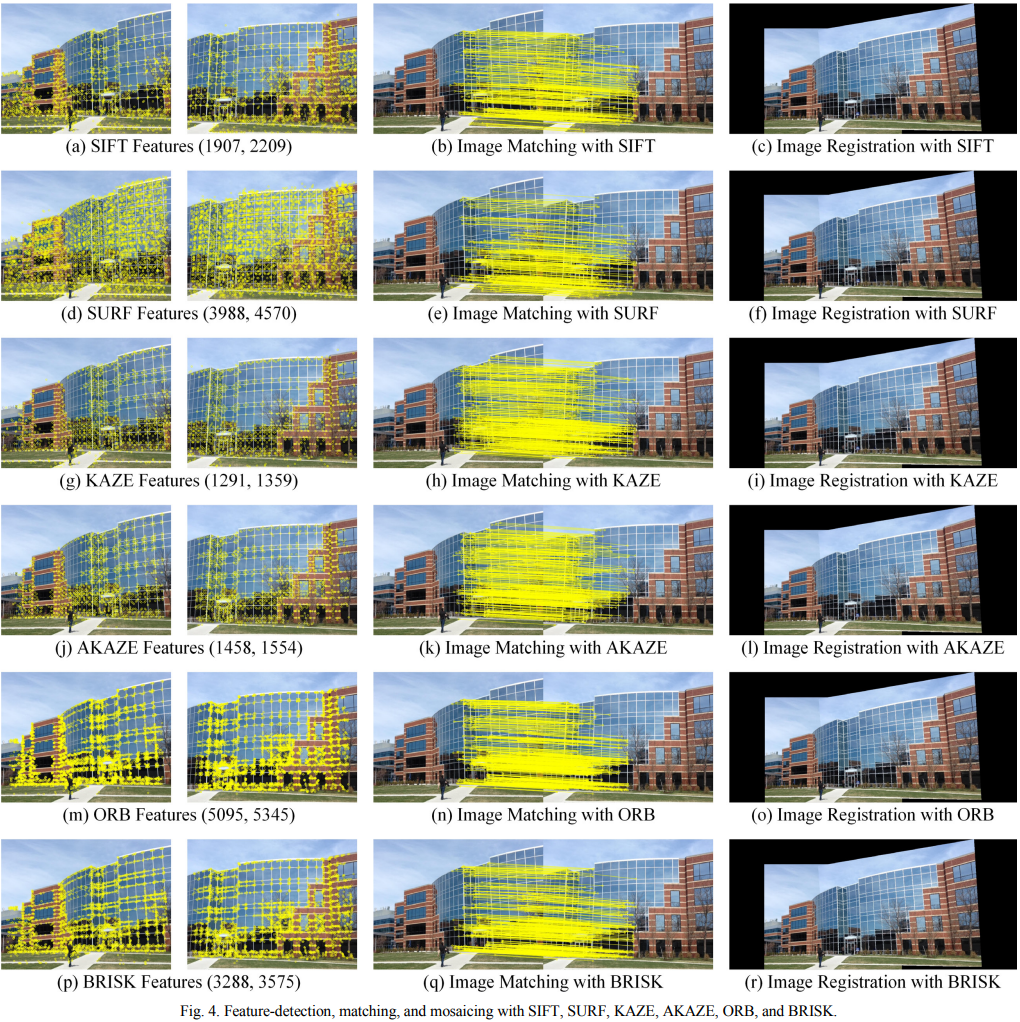
\includegraphics[width=0.85\textwidth]{image_detection}
  \caption{Merkmalsdetektion, Matching und Bildregistrierung derselben Szene mit
  SIFT, SURF, KAZE, AKAZE, ORB und BRISK (Zeilen). Die Detektoren unterscheiden
  sich deutlich in Anzahl und Verteilung der gefundenen Merkmale sowie in der
  Matching-Qualität; SIFT/AKAZE gelten als am genauesten, ORB/BRISK als am
  effizientesten. Nach \cite{tareen2018comparative}.}
  \label{fig:image_detection}
\end{figure}

\noindent \textbf{Faustregel für dieses Projekt:} ORB als Standardwahl für
Echtzeit-Matching und visuelle Odometrie, SIFT/AKAZE, wenn es bei der
CAD-Posenschätzung auf maximale Genauigkeit ankommt. Der folgende Code zeigt
die ORB-Variante exemplarisch.

\begin{lstlisting}[style=py,caption={ORB-Erkennung und Matching (klassisch, kein Training nötig)}]
import cv2

orb = cv2.ORB_create(nfeatures=1500)
# Referenzansicht des Bauteils (z.B. aus CAD-Render) einmalig beschreiben:
kp_ref, des_ref = orb.detectAndCompute(ref_gray, None)
matcher = cv2.BFMatcher(cv2.NORM_HAMMING)

def detect(frame_gray):
    kp, des = orb.detectAndCompute(frame_gray, None)
    if des is None:
        return []
    raw  = matcher.knnMatch(des_ref, des, k=2)
    good = [m for m, n in raw if m.distance < 0.75 * n.distance]  # Lowe
    return kp, good

# 6D-Pose ueber 2D-3D-Korrespondenzen (CAD-Punkte <-> Bildpunkte):
# ok, rvec, tvec = cv2.solvePnPRansac(obj_pts_3d, img_pts_2d,
#                                      K, distCoeffs)
\end{lstlisting}

\noindent Für \textbf{Bewegungserkennung} (Projekt~3) genügt
Hintergrundsubtraktion:
\begin{lstlisting}[style=py,caption={Bewegungserkennung ohne Merkmale}]
bg = cv2.createBackgroundSubtractorMOG2(detectShadows=False)
mask = bg.apply(frame)                      # bewegte Pixel
contours, _ = cv2.findContours(
    mask, cv2.RETR_EXTERNAL, cv2.CHAIN_APPROX_SIMPLE)
movers = [c for c in contours if cv2.contourArea(c) > 500]
\end{lstlisting}

% =============================================================
%  ch22a_echtzeit_scheduling.tex  --  Echtzeit-Stereoverarbeitung:
%  Zeitbudget, Frame-Dropping, Executor-Scheduling, Zustandsautomat
% =============================================================

\chapter{Echtzeit-Stereoverarbeitung: Scheduling, Frame-Dropping und Zustandsautomat}

Der Balltracker ist \textbf{zeitkritisch}: Bei 60\,fps hast du pro Frame nur
$\approx$\,16{,}7\,ms, um zu splitten, zu rektifizieren, den Ball in beiden
Bildern zu finden, zu triangulieren und den Kalman-Filter zu aktualisieren.
Dauert ein Frame länger, läuft die Verarbeitung der Realität hinterher. Dieses
Kapitel zeigt, wie man damit umgeht: Frames gezielt verwerfen, die Prädiktion von
der Messung entkoppeln und die Ablauflogik als Zustandsautomat strukturieren.

\section{Das Zeitbudget eines Frames}
Die Pipeline besteht aus Stufen mit je eigenem Latenzanteil:
\begin{longtable}{@{}p{6.0cm}p{3.0cm}p{5.0cm}@{}}
\toprule
\textbf{Stufe} & \textbf{typ.\ Latenz} & \textbf{Anmerkung} \\
\midrule
Belichtung + USB-Transfer & 2--8\,ms & von der Kamera vorgegeben \\
Split + Rektifizierung    & 1--3\,ms & einmalige Remap-LUT \\
Balldetektion (sparse, beide Bilder) & 2--10\,ms & der teure, schwankende Teil \\
Triangulation + KF-Update & $<$\,1\,ms & billig \\
\bottomrule
\end{longtable}

\noindent Es gibt \textbf{zwei verschiedene Fehlermodi}, die man nicht verwechseln
darf:
\begin{description}[style=nextline,leftmargin=1.4em]
\item[Latenz (zu alt).] Ein einzelner Frame ist verarbeitet, aber das Ergebnis
  kommt zu spät -- die Schätzung beschreibt einen vergangenen Ballort.
\item[Durchsatz (Stau).] Frames kommen schneller, als du sie verarbeitest. Ohne
  Gegenmaßnahme wächst die Warteschlange unbegrenzt, und die Latenz steigt mit
  jeder Sekunde weiter an (\emph{Bufferbloat}).
\end{description}

\begin{warnbox}[title=Die Kernregel für den Kalman-Filter]
Ein \textbf{veralteter} Messwert ist schlechter als \emph{gar kein} Messwert. Der
Filter kann über reine Prädiktion problemlos einige Frames überbrücken (vgl.\
Kalman-Knoten). Also: lieber den alten Frame \textbf{verwerfen} und auf den
nächsten aktuellen warten, als einen veralteten Messwert ins Update zu geben.
\textbf{Niemals Frames aufstauen.}
\end{warnbox}

\section{Frame-Dropping: DDS macht die Arbeit}
Der wichtigste Hebel ist die \textbf{QoS}: Mit \code{KEEP\_LAST}, Tiefe~1 und
\code{BEST\_EFFORT} verwirft DDS selbst alte Bilder -- während dein Callback
rechnet, überschreibt jeder neue Frame den wartenden, und du bekommst nach dem
Callback stets den \emph{neuesten} statt des nächst-ältesten. Genau das ist das
\code{sensor\_data}-QoS-Profil.

\begin{lstlisting}[style=py,caption={QoS für Bild-Topics: nur der neueste Frame zählt}]
from rclpy.qos import qos_profile_sensor_data
# entspricht: BEST_EFFORT + KEEP_LAST + depth=1
self.create_subscription(
    Image, '/left/image_raw', self.on_frame, qos_profile_sensor_data,
    callback_group=self.cb_detect)
\end{lstlisting}

\noindent\textbf{Warum nicht RELIABLE?} \code{RELIABLE} lässt DDS verlorene Frames
neu senden -- bei einem Hochfrequenz-Bildstrom erzeugt das genau den Rückstau,
den du vermeiden willst. \code{RELIABLE} gehört auf das \emph{Ergebnis} (die
3D-Ballposition), \code{BEST\_EFFORT} auf den Bildstrom.

\noindent Als zweite Verteidigungslinie verwirfst du im Callback explizit zu alte
Frames anhand des Zeitstempels -- das fängt auch den Fall ab, dass DDS dir doch
einen leicht veralteten Frame zustellt:
\begin{lstlisting}[style=py,caption={Stale-Gating: Frame anhand seines Alters verwerfen}]
def on_frame(self, msg):
    now   = self.get_clock().now()
    stamp = rclpy.time.Time.from_msg(msg.header.stamp)
    age_s = (now - stamp).nanoseconds * 1e-9
    if age_s > self.max_age_s:          # z. B. 0.020 s = ein Frame bei 60 fps
        self.dropped += 1
        return                          # verwerfen statt verspaetet verarbeiten
    self.process(msg)                   # detektieren -> triangulieren -> KF-Update
\end{lstlisting}

\section{Scheduling: Executor und Callback-Gruppen}
Standardmäßig serialisiert der \code{SingleThreadedExecutor} alle Callbacks: ein
langsamer Detektions-Callback \textbf{blockiert dann auch den Prädiktions-Timer}.
Für zeitkritischen Code trennst du die Anliegen über einen
\code{MultiThreadedExecutor} und \textbf{Callback-Gruppen}:
\begin{itemize}
\item \code{MutuallyExclusiveCallbackGroup}: Callbacks dieser Gruppe laufen nie
  gleichzeitig -- richtig für den CPU-gebundenen Detektor (eine Instanz zur Zeit,
  zusammen mit Tiefe~1 ergibt das automatisches Frame-Dropping).
\item Ein \emph{eigener} Timer-Callback in einer \emph{eigenen} Gruppe für die
  Prädiktion -- so läuft sie in festem Takt weiter, selbst während die Detektion
  noch an einem Frame rechnet.
\end{itemize}

\begin{lstlisting}[style=py,caption={Prädiktion und Detektion in getrennten Gruppen, parallel ausgeführt}]
from rclpy.executors import MultiThreadedExecutor
from rclpy.callback_groups import MutuallyExclusiveCallbackGroup

class Perception(Node):
    def __init__(self):
        super().__init__('perception')
        self.cb_detect  = MutuallyExclusiveCallbackGroup()   # teuer, schwankend
        self.cb_predict = MutuallyExclusiveCallbackGroup()   # billig, deterministisch
        self.create_subscription(Image, '/left/image_raw', self.on_frame,
                                 qos_profile_sensor_data, callback_group=self.cb_detect)
        self.create_timer(1/120.0, self.predict, callback_group=self.cb_predict)

def main():
    rclpy.init()
    node = Perception()
    ex = MultiThreadedExecutor(num_threads=3)   # detect | predict | reserve
    ex.add_node(node); ex.spin()
\end{lstlisting}

\noindent\textbf{Prädiktion schneller als die Kamera.} Der Predict-Timer darf
ruhig mit 120\,Hz laufen, obwohl die Kamera nur 60\,fps liefert -- Prädiktion ist
billig und liefert zwischen den Messungen eine glatte, aktuelle Schätzung. Die
Messung (Update) kommt ereignisgesteuert, wann immer ein \emph{frischer}
Frame durchkommt. Das ist genau die Predict/Update-Aufteilung aus dem Kalman-Knoten,
nur sauber auf zwei Threads gelegt.

\begin{infobox}[title=Veraltete und vertauschte Messungen (Out-of-Order)]
Kommt eine Messung mit einem Zeitstempel \emph{vor} dem aktuellen Filterstand an
(z.\,B.\ weil ein langsamer Detektions-Thread sie spät abliefert), sind zwei
Wege sauber: (a) sie schlicht \textbf{verwerfen} (einfach, meist ausreichend),
oder (b) ein \textbf{Out-of-Sequence-Update} -- Filter auf den Mess-Zeitpunkt
zurückrollen, einarbeiten, wieder vorrollen. Für den Tischtennisball reicht~(a).
Hilfreich, wenn linkes/rechtes Bild synchron sein müssen:
\code{message\_filters.ApproximateTimeSynchronizer}.
\end{infobox}

\section{Ablauflogik als Zustandsautomat}
Die Frage ``was tue ich pro Frame'' hängt vom \textbf{Zustand} ab: Solange kein
Ball da ist, suchst du; sobald genug Punkte einer Flugbahn vorliegen, rechnest du
den Auftreffpunkt; ist der Schlag ausgelöst, fährst du ihn ab. Diese Logik
gehört nicht verstreut in den Bild-Callback, sondern in einen expliziten
\textbf{Zustandsautomaten}, der die Wahrnehmungs-Rate von der Entscheidungs-Rate
entkoppelt.

\begin{center}
\begin{tikzpicture}[node distance=15mm,every node/.style={font=\scriptsize}]
\node[node] (s) {SEARCH\\\scriptsize jeden Frame, Ball suchen};
\node[node,right=of s] (t) {TRACK\\\scriptsize KF-Update, Flugbahn sammeln};
\node[node,right=of t] (i) {INTERCEPT\\\scriptsize Auftreffpunkt prädizieren};
\node[node,below=10mm of i] (st) {STRIKE\\\scriptsize Trajektorie ausführen};
\node[node,left=of st] (r) {RECOVER\\\scriptsize zurück in Grundstellung};
\draw[flow] (s) -- node[topic,fill=white,inner sep=1pt]{\scriptsize Ball erkannt} (t);
\draw[flow] (t) -- node[topic,fill=white,inner sep=1pt]{\scriptsize genug Punkte} (i);
\draw[flow] (i) -- node[topic,fill=white,inner sep=1pt]{\scriptsize Schlagebene erreicht} (st);
\draw[flow] (st) -- node[topic,fill=white,inner sep=1pt]{\scriptsize Schlag fertig} (r);
\draw[flow] (r) -- node[topic,fill=white,inner sep=1pt]{\scriptsize bereit} (s);
\draw[flow] (t) to[bend left=20] node[topic,fill=white,inner sep=1pt]{\scriptsize Ball verloren} (s);
\end{tikzpicture}
\captionof{figure}{Zustandsautomat des Balltrackers. Die Stereo-Detektion treibt
die Übergänge; die Prädiktion läuft zustandsübergreifend im eigenen Timer weiter.}
\end{center}

\noindent\textbf{Umsetzung in ROS\,2 -- drei Stufen nach Komplexität:}
\begin{description}[style=nextline,leftmargin=1.4em]
\item[Eigenes \code{Enum} im Knoten.] Für eine überschaubare Logik wie diese das
  Pragmatischste: ein Zustandsfeld plus \code{match}/\code{if}. Kein Framework,
  voll unter Kontrolle.
\item[YASMIN.] ROS\,2-native Zustandsmaschinen-Bibliothek (Python/C++) mit
  Introspektion -- sinnvoll, wenn die Zustände wachsen.
\item[Behavior Trees.] \code{BehaviorTree.CPP} (wie in Nav2) oder
  \code{py\_trees\_ros} -- für komplexe, wiederverwendbare Verhaltensbäume mit
  Fallbacks; für den reinen Balltracker meist überdimensioniert.
\end{description}

\begin{lstlisting}[style=py,caption={Zustandsautomat als Enum -- Entscheidung getrennt vom Bild-Callback}]
from enum import Enum, auto

class S(Enum):
    SEARCH = auto(); TRACK = auto(); INTERCEPT = auto(); STRIKE = auto(); RECOVER = auto()

class Brain(Node):
    def __init__(self, kf):
        super().__init__('brain')
        self.kf = kf; self.state = S.SEARCH; self.hits = 0
        # eigener Takt: Entscheidung entkoppelt von der Frame-Rate
        self.create_timer(1/200.0, self.tick)

    def on_measurement(self, ok):          # vom Detektor pro frischem Frame
        self.hits = self.hits + 1 if ok else 0

    def tick(self):
        if self.state is S.SEARCH and self.hits > 0:
            self.state = S.TRACK
        elif self.state is S.TRACK:
            if self.hits == 0:                       self.state = S.SEARCH   # Ball verloren
            elif self.hits >= self.min_track:        self.state = S.INTERCEPT
        elif self.state is S.INTERCEPT:
            p = self.kf.predict_intercept(self.z_plane)   # reine Praediktion
            if p is not None:
                self.send_goal(p); self.state = S.STRIKE
        elif self.state is S.STRIKE and self.motion_done():
            self.state = S.RECOVER
        elif self.state is S.RECOVER and self.at_home():
            self.hits = 0; self.state = S.SEARCH
\end{lstlisting}

\begin{infobox}[title=Das Architektur-Prinzip in einem Satz]
Drei entkoppelte Takte statt einer verschachtelten Schleife: \textbf{Detektion}
(ereignisgesteuert, verwirft alte Frames per QoS), \textbf{Prädiktion}
(schneller Timer, läuft immer), \textbf{Entscheidung} (eigener Timer, fährt den
Zustandsautomaten) -- über einen \code{MultiThreadedExecutor} mit getrennten
Callback-Gruppen, damit kein langsamer Frame die anderen beiden blockiert.
\end{infobox}


% =============================================================
% TEIL III  --  Hardware-Auswahl
% =============================================================
\part{Hardware-Auswahl}

% =============================================================
%  ch08_komponenten.tex  --  Komponenten im günstigen Hobby-Bereich
% =============================================================

\chapter{Komponenten im günstigen Hobby-Bereich}

\begin{infobox}[title=Leitprinzip]
Fokus liegt nicht auf Elektrotechnik: Wo möglich Module und Plug-and-Play,
niedrige Kosten. Die Architektur trennt sauber eine
\textbf{Echtzeit-Motorebene} (Mikrocontroller, nah an den Treibern) von einer
\textbf{High-Level-Ebene} (PC/Pi mit vollem ROS\,2 für Trajektorie, Vision,
Kalman).
\end{infobox}

\section{Schrittmotor und Treiber}
\begin{longtable}{@{}p{3.6cm}p{4.2cm}p{7.2cm}@{}}
\toprule
\textbf{Komponente} & \textbf{Empfehlung} & \textbf{Begründung} \\
\midrule
Motor          & NEMA-17 (z.\,B.\ 17HS19) & Standard, günstig, ausreichend Moment mit Getriebe \\
Treiber        & \textbf{TMC2209} (UART)   & StallGuard4 liefert Lastwert über UART = indirekte Drehmomentschätzung; leise, Stepstick-Format, $\approx$5--10\,\euro \\
Treiber-Alt.   & TMC2130/5160 (SPI)       & höherer Strom / SPI statt UART \\
Strom/Spannung & \textbf{INA226}-Modul (I\textsuperscript{2}C) & misst Busspannung + Strom direkt, plug-and-play, $\approx$2\,\euro\ pro Kanal \\
Closed-Loop (opt.) & MKS SERVO42 / BTT S42B & integrierter Encoder + Treiber, falls echter Regelkreis gewünscht \\
\bottomrule
\end{longtable}

\noindent\textbf{Konkret für den Regelungsansatz:} Der TMC2209 im UART-Modus
gibt \code{SG\_RESULT} (Lastproxy) ohne Zusatzhardware. Willst du
\emph{zusätzlich} Busspannung und -strom explizit messen, setzt du je Achse ein
INA226-Modul auf die Treiberversorgung. Beide hängen am selben I\textsuperscript{2}C/UART-Bus
des Mikrocontrollers.

\section{Recheneinheiten}
\begin{description}[style=nextline,leftmargin=1.4em]
\item[ESP32 (Motorebene)] Dual-Core, viele PWM/GPIO, FreeRTOS, harte Echtzeit
  für Schrittgenerierung und das Auslesen von TMC (UART) und INA226
  (I\textsuperscript{2}C). Entscheidend: \textbf{micro-ROS} bindet den ESP32
  als vollwertigen ROS\,2-Knoten in den Graphen ein.
\item[Raspberry Pi (High-Level)] Pi\,4/5 mit Ubuntu kann den vollen
  ROS\,2-Stack tragen (Trajektorienplanung, Kalman). Der \textbf{Pi Zero} ist
  dafür zu schwach -- für Vision ungeeignet; nutze ihn höchstens als
  micro-ROS-Brücke. Vision und schweres Rechnen gehören auf den externen PC.
\end{description}

\begin{infobox}[title=Empfohlene Arbeitsteilung]
\textbf{Externer PC} (Ubuntu + ROS\,2): Trajektorienplanung, Stereo-Vision,
Kalman-Filter, Visualisierung.
\;$\longleftrightarrow$\; (WLAN/USB) \;$\longleftrightarrow$\;
\textbf{ESP32} (micro-ROS): empfängt Sollwerte, generiert Schritte, liest
StallGuard/INA226, publiziert Gelenkzustände. Die Stereokamera hängt per USB
am PC.
\end{infobox}

\section{Stereokamera}
Das ELP-Modell ist eine synchronisierte Doppelobjektiv-USB-Kamera
(UVC-konform). Sie meldet sich unter Linux als V4L2-Gerät (\code{/dev/video*})
und liefert in der Regel ein \emph{nebeneinanderliegendes} (side-by-side) Bild
über eine USB-Verbindung -- die Synchronisierung beider Sensoren ist der
Vorteil gegenüber zwei Einzelkameras (wichtig für bewegte Objekte wie den Ball).
In ROS\,2:
\begin{itemize}
\item Treiber: \code{v4l2\_camera} oder \code{usb\_cam}.
\item Side-by-side-Frame in linkes/rechtes Bild splitten (kleiner eigener Knoten,
  siehe Teil~VI).
\item Eigene Stereokalibrierung ist Pflicht -- das Modul ist nicht vorkalibriert.
\end{itemize}

% =============================================================
%  ch09_pcb.tex  --  Optimierungspotenzial für ein eigenes PCB
% =============================================================

\chapter{Optimierungspotenzial für ein eigenes PCB}

Diese Punkte sind \emph{Erweiterung}, nicht Voraussetzung -- mit Modulen kommst
du zunächst aus. Für ein späteres eigenes Board:
\begin{itemize}
\item \textbf{Treiber integrieren} statt Stepstick-Module: TMC2209 direkt
  bestücken -- spart Bauhöhe, bessere Thermik über Kupferflächen und Thermovias
  unter dem Chip.
\item \textbf{Strom-/Spannungsmessung onboard:} INA-Sensor mit dimensioniertem
  Shunt je Kanal nahe am Treiber, kurze Kelvin-Anbindung des Shunts.
\item \textbf{Power-Integrity:} Bulk-Elko plus keramische Stützkondensatoren
  direkt an jedem Treiber; getrennte Power-/Logik-Masse mit Sternpunkt
  (Single-Point-Ground).
\item \textbf{Signalführung:} STEP/DIR bzw.\ UART als kurze, von der Leistung
  getrennte Leitungen; bei gemischten Pegeln (3{,}3\,V/5\,V) Levelshifter
  vorsehen.
\item \textbf{Schutz:} ESD-Dioden an USB- und Encoder-Leitungen; Verpolschutz;
  Freilauf-/EMV-Betrachtung der Motorleitungen.
\item \textbf{Konnektivität:} JST-Stecker für Motoren/Encoder, Schraubklemme
  für die Versorgung; optional CAN-Transceiver für saubere
  Mehrachs-Verkettung statt vieler UARTs.
\item \textbf{Onboard-Encoder-Interface} für späteren Closed-Loop-Betrieb (FOC).
\item \textbf{Thermik:} Thermopad/Kühlfläche unter den Treibern, definierter
  Luftstrom.
\end{itemize}


% =============================================================
% TEIL IV  --  Software-Setup: VM, Linux, ROS 2
% =============================================================
\part{Software-Setup: VM, Linux, ROS\,2}

% =============================================================
%  ch10_betriebssystem.tex  --  Betriebssystem und Distribution
% =============================================================

\chapter{Betriebssystem und Distribution}

\section{Distributionswahl (Stand Juni 2026)}
ROS\,2-Releases erscheinen jährlich; relevant sind die LTS-Versionen. Für ein
langfristiges Lernprojekt:
\begin{longtable}{@{}p{3.4cm}p{2.6cm}p{2.4cm}p{6cm}@{}}
\toprule
\textbf{Distribution} & \textbf{Ubuntu} & \textbf{Support bis} & \textbf{Eignung} \\
\midrule
\textbf{Jazzy Jalisco} & 24.04 & 2029 (LTS) & \textbf{Empfehlung}: reif, viele Tutorials, von Isaac Sim unterstützt \\
Humble Hawksbill       & 22.04 & 2027 (LTS) & meiste Tutorials, etwas älter \\
Kilted Kaiju           & 24.04 & $\sim$2026 & non-LTS, kurzer Support -- meiden \\
Lyrical Luth           & 24.04 & 2031 (LTS) & brandneu (Mai 2026), Ökosystem noch nicht nachgezogen \\
\bottomrule
\end{longtable}

\begin{infobox}[title=Empfehlung]
\textbf{Ubuntu 24.04 LTS + ROS\,2 Jazzy Jalisco.} LTS bis 2029, ausgereifte
Tutorials, von Gazebo Harmonic und NVIDIA Isaac Sim unterstützt. Lyrical Luth
ist erst $\sim$10 Tage alt -- für den Einstieg zu frisch.
\end{infobox}

\section{VM, Dual-Boot oder WSL2?}
\begin{warnbox}[title=Wichtige Einschränkung bei der VM]
Eine VM (VirtualBox/VMware) ist für die \emph{ROS\,2-Grundlagen} in Ordnung,
aber \textbf{Gazebo Harmonic und Isaac Sim brauchen GPU-Beschleunigung}, die in
VMs schlecht durchgereicht wird -- 3D-Simulation läuft dort zäh. Optionen,
nach Eignung:
\begin{enumerate}
\item \textbf{Natives Ubuntu (Dual-Boot)} -- beste Leistung, empfohlen sobald du
  simulierst.
\item \textbf{WSL2 unter Windows} -- inzwischen mit GPU-Zugriff (WSLg), guter
  Kompromiss.
\item \textbf{VM} -- nur für CLI/Tutorials; für schwere Simulation ungeeignet.
\end{enumerate}
\end{warnbox}

% =============================================================
%  ch11_installation.tex  --  ROS 2 installieren (Schritt für Schritt)
% =============================================================

\chapter{ROS\,2 installieren -- Schritt für Schritt}

\begin{lstlisting}[style=bash,caption={Locale + ROS\,2-Apt-Quelle (Ubuntu 24.04)}]
# 1) Locale auf UTF-8
sudo apt update && sudo apt install -y locales
sudo locale-gen en_US en_US.UTF-8
sudo update-locale LC_ALL=en_US.UTF-8 LANG=en_US.UTF-8

# 2) Universe-Repo + Schluessel + ROS2-Quelle
sudo apt install -y software-properties-common curl
sudo add-apt-repository universe
sudo curl -sSL https://raw.githubusercontent.com/ros/rosdistro/master/ros.key \
  -o /usr/share/keyrings/ros-archive-keyring.gpg
echo "deb [arch=$(dpkg --print-architecture) \
  signed-by=/usr/share/keyrings/ros-archive-keyring.gpg] \
  http://packages.ros.org/ros2/ubuntu \
  $(. /etc/os-release && echo $UBUNTU_CODENAME) main" \
  | sudo tee /etc/apt/sources.list.d/ros2.list > /dev/null
sudo apt update
\end{lstlisting}

\begin{lstlisting}[style=bash,caption={ROS\,2 Jazzy + Entwicklungswerkzeuge}]
# 3) ROS2 Desktop (inkl. RViz2, Demos)
sudo apt install -y ros-jazzy-desktop

# 4) Build-Werkzeuge
sudo apt install -y ros-dev-tools \
  python3-colcon-common-extensions python3-rosdep
sudo rosdep init && rosdep update

# 5) In jeder Shell verfuegbar machen
echo "source /opt/ros/jazzy/setup.bash" >> ~/.bashrc && source ~/.bashrc

# 6) Funktionstest (zwei Terminals)
ros2 run demo_nodes_cpp talker      # Terminal A
ros2 run demo_nodes_py listener     # Terminal B
\end{lstlisting}

\section{Pakete, die du für die Projekte brauchst}
\begin{longtable}{@{}p{6.2cm}p{8.6cm}@{}}
\toprule
\textbf{Paket (apt: \code{ros-jazzy-...})} & \textbf{Zweck} \\
\midrule
\code{ros-gz} (Gazebo Harmonic Bridge)      & Simulation $\leftrightarrow$ ROS\,2 \\
\code{ros2-control}, \code{ros2-controllers}& Hardware-Abstraktion, \code{joint\_trajectory\_controller} \\
\code{gz-ros2-control}                      & ros2\_control-Plugin für Gazebo \\
\code{moveit}                               & Bewegungsplanung, IK, Greifen (Projekt~4) \\
\code{navigation2}, \code{nav2-bringup}     & Autonome Navigation (Projekt~3) \\
\code{slam-toolbox}                         & SLAM/Kartierung (Projekt~3) \\
\code{robot-localization}                   & EKF/UKF-Sensorfusion (Odometrie) \\
\code{image-pipeline}                       & \code{camera\_calibration}, \code{stereo\_image\_proc} \\
\code{v4l2-camera} bzw.\ \code{usb-cam}     & Treiber für die USB-Stereokamera \\
\code{vision-opencv} (\code{cv\_bridge})    & OpenCV $\leftrightarrow$ ROS\,2-Bildnachrichten \\
\code{xacro}, \code{robot-state-publisher}  & URDF/Xacro, TF-Veröffentlichung \\
\code{rqt}, \code{rqt-graph}, \code{rqt-image-view} & Introspektion/Visualisierung \\
\bottomrule
\end{longtable}
\noindent Installation gebündelt, z.\,B.\
\code{sudo apt install ros-jazzy-ros-gz ros-jazzy-ros2-control ros-jazzy-moveit \ldots}\
Für den ESP32 zusätzlich der \textbf{micro-ROS Agent} (separat aus dem
micro-ROS-Workspace gebaut).


% =============================================================
% TEIL V  --  Simulation und der Weg vom CAD-Modell zur Realität
% =============================================================
\part{Simulation und der Weg vom CAD-Modell zur Realität}

% =============================================================
%  ch12_simulationswerkzeuge.tex  --  Simulationswerkzeuge im ROS 2-Ökosystem
% =============================================================

\chapter{Simulationswerkzeuge im ROS\,2-Ökosystem}

\textbf{Gazebo Classic ist seit Januar 2025 EOL}; ``modernes Gazebo''
(früher Ignition) ist der Nachfolger:
\begin{longtable}{@{}p{3.2cm}p{4.4cm}p{7.4cm}@{}}
\toprule
\textbf{Werkzeug} & \textbf{Charakter} & \textbf{Eignung} \\
\midrule
\textbf{Gazebo Harmonic} & Standard-Simulator für Jazzy, Bridge \code{ros\_gz} & Allrounder: Physik, Sensoren (Kamera, Tiefe, IMU, LiDAR), \code{gz\_ros2\_control}. \textbf{Erste Wahl.} \\
NVIDIA Isaac Sim         & photorealistisch, GPU & Vision/Pose-Schätzung mit realistischen Bildern; braucht starke GPU; nur LTS-Distros \\
Webots                   & einfach, didaktisch    & schneller Einstieg, gute ROS\,2-Anbindung \\
MuJoCo                   & schnelle, präzise Dynamik & kontaktreiche Regelung, RL; weniger Sensor-Realismus \\
PyBullet                 & leichtgewichtig        & schnelles Prototyping von Kinematik/Dynamik \\
\bottomrule
\end{longtable}
\noindent \textbf{RViz2} ist kein Simulator, sondern Visualisierung -- du nutzt
es parallel.

\section{Was lässt sich vorab simulieren?}
Sehr viel -- die meiste \emph{Logik} der vier Projekte ist simulierbar:
\begin{itemize}
\item \textbf{Kinematik/Dynamik} des Stepper-Roboters: Gelenkbewegung,
  Trajektorienabfahrt, Kollisionen, Massen/Trägheiten.
\item \textbf{Sensoren:} simulierte Stereokamera (gerenderte Bilder -- du kannst
  deine Merkmalserkennung darauf testen), Tiefenbild, IMU, LiDAR, Odometrie.
\item \textbf{Tischtennisball:} Projektilflug inkl.\ Gravitation und Aufprall
  als Starrkörperphysik; dein Kalman-Filter kann auf den simulierten
  3D-Positionen laufen.
\item \textbf{Navigation:} Nav2 + simulierte Odometrie/LiDAR in einer Welt.
\item \textbf{Greifen:} MoveIt\,2-Planung in simulierter Szene mit platzierten
  Bauteilen.
\end{itemize}

\begin{infobox}[title=Kannst du die Projekte vollständig in Simulation umsetzen?]
\textbf{Die Steuerungs-, Planungs- und Wahrnehmungs-Logik: ja.} Du kannst
Trajektorienregelung, Kalman-Schätzung, Navigation und die Vision-Pipeline
komplett in Gazebo entwickeln und testen. \textbf{Was die Simulation nicht
abbildet:} reales Kamerarauschen/Kalibrierfehler, Schrittverluste und
Resonanzen des realen Steppers, exakte Kontaktdynamik (Ballspin/-absprung sind
Näherungen), reale Latenzen und Zeitverhalten. Diese Effekte treten erst auf
der echten Hardware zutage.
\end{infobox}

% =============================================================
\section{MuJoCo und Isaac Sim im Detail}
Zwei Werkzeuge der obigen Tabelle verdienen eine genauere Betrachtung, weil sie
in der modernen Robotik -- besonders im Lernen von Regelungen
(\emph{Reinforcement Learning}, RL) und in der Wahrnehmung -- eine
Sonderstellung einnehmen. Sie lösen Probleme, an denen Gazebo als
Allzweck-Simulator an seine Grenzen stößt: \textbf{MuJoCo} bei der schnellen,
präzisen Kontaktdynamik, \textbf{Isaac Sim} beim photorealistischen Rendern und
beim massiv parallelen GPU-Training.

\subsection{MuJoCo -- Multi-Joint dynamics with Contact}
\textbf{MuJoCo} (\emph{Multi-Joint dynamics with Contact}) ist eine
quelloffene Physik-Engine, ursprünglich 2012 von Emanuel Todorov vorgestellt
\cite{todorov2012mujoco} und seit 2021 von Google DeepMind entwickelt und unter
Apache-2.0 frei verfügbar \cite{mujoco_docs}. Ihr Markenzeichen ist ein
\textbf{stabiler, weicher Kontaktlöser} (konvexe Optimierung pro Zeitschritt),
der kontaktreiche Vorgänge -- Greifen, Laufen, Anschlagen -- numerisch stabil
und schnell rechnet.

\begin{itemize}
\item \textbf{Stärken:} sehr schnelle und genaue Dynamik (oft schneller als
  Echtzeit, hunderte bis tausende Schritte/s), differenzierbare Physik,
  analytisch saubere Gelenk-/Sehnenmodelle, exzellent für Regelungs- und
  RL-Forschung. Mit \textbf{MJX} läuft MuJoCo über JAX auf der GPU und
  simuliert tausende Welten parallel.
\item \textbf{Schwächen:} \emph{kein} photorealistisches Rendering (einfacher
  OpenGL-Viewer), weniger fertige Sensor-Plugins als Gazebo, Modelle in eigenem
  \code{MJCF}-XML (URDF-Import möglich, aber oft mit Nacharbeit).
\item \textbf{Robotik-Relevanz:} De-facto-Standard im RL-Benchmarking
  (\code{Gymnasium}/\code{dm\_control}), Lokomotion vierbeiniger Roboter,
  geschickte Manipulation, Modellprädiktive Regelung (MPC). Wenn die
  \emph{Kontaktphysik} und die \emph{Trainingsgeschwindigkeit} zählen, ist
  MuJoCo erste Wahl.
\end{itemize}

\subsection{NVIDIA Isaac Sim -- photorealistisch und GPU-parallel}
\textbf{Isaac Sim} ist NVIDIAs Robotik-Simulator auf Basis der
\textbf{Omniverse}-Plattform und des \code{USD}-Szenenformats
\cite{isaacsim_docs}. Die Physik liefert \textbf{PhysX\,5} (GPU-beschleunigt),
das Rendering nutzt \textbf{RTX-Raytracing} -- also physikalisch plausibles
Licht, Schatten und Materialien.

\begin{itemize}
\item \textbf{Stärken:} \emph{photorealistische} Kamerabilder, exzellente
  Erzeugung synthetischer Trainingsdaten (\emph{Synthetic Data}, inkl.\
  automatischer Labels: Segmentierung, Bounding-Boxes, Tiefe), \emph{Domain
  Randomization} für robuste Vision-Modelle, GPU-parallele Physik für
  großskaliges RL über \textbf{Isaac Lab} \cite{mittal2023isaaclab}.
\item \textbf{Schwächen:} braucht eine starke NVIDIA-RTX-GPU (VRAM-hungrig),
  hohe Einstiegshürde, große Installation; weniger ``leichtgewichtig'' als
  Gazebo oder MuJoCo für schnelle Iteration.
\item \textbf{Robotik-Relevanz:} überall dort, wo das \emph{Aussehen} der Szene
  entscheidend ist -- Training von Objekterkennung/Pose-Schätzung, Sim-to-Real
  für kamerabasierte Politiken, digitale Zwillinge ganzer Fertigungszellen.
\end{itemize}

% =============================================================
\section{Lassen sie sich integriert einsetzen?}
\textbf{Ja -- aber meist arbeitsteilig, nicht als ein gemeinsamer
Simulationskern.} Beide sprechen ROS\,2, sodass sie sich in dieselbe Knoten- und
Topic-Architektur einfügen wie Gazebo. Der gemeinsame Nenner ist wieder
\code{ros2\_control} (vgl.\ das folgende Kapitel zur Sim-Real-Trennung): die
High-Level-Logik bleibt identisch, nur die unterste Schicht -- der Simulator
hinter dem Hardware-Interface -- wird getauscht.

\begin{longtable}{@{}p{3.0cm}p{5.4cm}p{6.6cm}@{}}
\toprule
\textbf{Werkzeug} & \textbf{ROS\,2-Anbindung} & \textbf{Typische Rolle im Workflow} \\
\midrule
Gazebo Harmonic & \code{ros\_gz}-Bridge, \code{gz\_ros2\_control} & Allround-Integrationstest, Sensorik, Nav2/MoveIt2 \\
MuJoCo          & \code{mujoco\_ros2\_control}, eigene Bridges    & Regler-/RL-Training, Kontaktdynamik, MPC \\
Isaac Sim       & natives \code{ROS\,2-Bridge}-Extension         & Vision-Trainingsdaten, photorealistische Pose-Schätzung, RL via Isaac Lab \\
\bottomrule
\end{longtable}

\noindent Der heute verbreitete \textbf{kombinierte Workflow} sieht so aus:
\begin{enumerate}
\item \textbf{Politik/Regler lernen} -- massiv parallel in \textbf{Isaac Lab}
  (auf Isaac Sim) oder in \textbf{MuJoCo/MJX} auf der GPU. Hier zählen
  Geschwindigkeit und Kontaktphysik, nicht das Aussehen.
\item \textbf{Wahrnehmung trainieren} -- photorealistische, automatisch
  gelabelte Bilder aus \textbf{Isaac Sim} für die Objekt-/Pose-Erkennung
  (Domain Randomization gegen den Sim-to-Real-Gap).
\item \textbf{Integrieren und gegentesten} -- die fertigen Knoten im
  \textbf{Gazebo}-Allroundmodell oder direkt am realen Roboter über
  \code{ros2\_control} verifizieren.
\end{enumerate}

\begin{infobox}[title=Einordnung für dieses Projekt]
Für den Stepper- und Tischtennisroboter ist \textbf{Gazebo Harmonic die
praktische Basis}: Kinematik, Sensorik, Kontakt Ball/Schläger, ros2\_control.
\textbf{MuJoCo} lohnt sich, falls die
\emph{Schlag-/Kontaktdynamik} oder eine \emph{gelernte Schlagpolitik}
(RL) genauer untersucht werden soll -- es rechnet kontaktreiche Vorgänge
schneller und stabiler. \textbf{Isaac Sim} wird relevant, wenn die
\emph{Ballerkennung} mit photorealistischen, gelabelten Bildern trainiert
werden soll, statt sie nur an realen Kamerabildern abzustimmen. Beide setzen
voraus: MuJoCo profitiert von einer GPU (MJX), Isaac Sim \emph{erfordert} eine
starke NVIDIA-RTX-GPU -- das ist die wichtigste Hürde gegenüber dem leichten
Gazebo-Setup.
\end{infobox}

% =============================================================
%  ch13_sim_real_trennung.tex  --  Wo sich Simulation und Realität trennen
% =============================================================

\chapter{Wo sich Simulation und reale Implementierung trennen}

Das ist die architektonisch wichtigste Einsicht des ganzen Dokuments. Der Trick
von \textbf{ros2\_control}: deine High-Level-Knoten (Trajektorienplaner, Vision,
Kalman, Nav2) bleiben \emph{identisch}. Was sich ändert, ist nur die unterste
Schicht -- das \textbf{Hardware-Interface-Plugin}.

\begin{center}
\begin{tikzpicture}[node distance=8mm]
\node[node,fill=accent!8] (high)
  {High-Level-Knoten\\\scriptsize Trajektorie $\cdot$ Vision $\cdot$ Kalman $\cdot$ Nav2 $\cdot$ MoveIt2};
\node[node,below=of high] (ctrl)
  {controller\_manager\\\scriptsize joint\_trajectory\_controller, joint\_state\_broadcaster};
\node[node,below left=10mm and -10mm of ctrl,fill=accent!18] (sim)
  {Sim-Hardware-Interface\\\scriptsize gz\_ros2\_control};
\node[node,below right=10mm and -10mm of ctrl,fill=accent2!12,draw=accent2] (real)
  {Reales Hardware-Interface\\\scriptsize micro-ROS / Serial $\rightarrow$ ESP32 $\rightarrow$ TMC2209};
\node[node,below=8mm of sim] (gz)
  {Gazebo Harmonic\\\scriptsize Physik + Sensoren};
\node[node,below=8mm of real,draw=accent2,fill=accent2!8] (hw)
  {Realer Roboter\\\scriptsize Motoren, Encoder, Kamera};
\draw[flow] (high)--(ctrl);
\draw[flow] (ctrl)--(sim);
\draw[flow] (ctrl)--(real);
\draw[flow] (sim)--(gz);
\draw[flow] (real)--(hw);
\node[font=\scriptsize\itshape,accent] at ($(high)+(6.4,0)$)
  {\;identisch in Sim \& Real};
\end{tikzpicture}
\captionof{figure}{Sim-zu-Real: nur die unterste Schicht (Hardware-Interface)
wird getauscht. Alles darüber bleibt gleich.}
\end{center}

\noindent Konkret: In der Simulation lädt die URDF das Plugin
\code{gz\_ros2\_control/GazeboSimSystem}. Für die echte Maschine schreibst du
ein eigenes \code{hardware\_interface::SystemInterface}, das Sollwerte an den
ESP32 schickt (micro-ROS oder serielle Brücke) und Gelenkzustände
(Encoder/StallGuard) zurückliest. \textbf{Dieselben Controller, dieselben
Topics, dieselbe Trajektorie} -- du tauschst eine Plugin-Zeile und die
Hardware. Genauso bei der Kamera: simulierte Bildquelle vs.\ \code{v4l2\_camera}
-- die nachgelagerte Vision-Pipeline merkt keinen Unterschied.

% =============================================================
%  ch14_cad_urdf.tex  --  Vorabschritte: vom CAD-Modell zur Simulation
% =============================================================

\chapter{Vorabschritte: vom CAD-Modell zur Simulation}
\label{ch:cad_urdf}

Bevor du simulierst, brauchst du ein \textbf{URDF} (Unified Robot Description
Format) -- die XML-Beschreibung deines Roboters aus \emph{Links} (starre
Körper) und \emph{Joints} (Gelenke dazwischen).

\section{Getrennte STL-Exporte pro Gelenk}
Wenn zwischen Teil\,A und Teil\,B eine Gelenkverbindung besteht, müssen beide
\emph{separat} als Mesh (STL/DAE) exportiert werden -- denn jedes ist ein
eigener Link mit eigenem Koordinatensystem, und das Gelenk dazwischen wird in
der URDF definiert, nicht im CAD-Mesh. Vorgehen:
\begin{enumerate}
\item Im CAD die Gelenkachsen und je Link ein Referenz-Frame festlegen
  (idealerweise Mesh-Ursprung = Gelenkpunkt -- erspart später viel Frame-Frust).
\item \textbf{Jeden Link einzeln} als STL exportieren (Teil\,A, Teil\,B,
  \dots), bevorzugt in seinem eigenen Frame.
\item Masse + Trägheitstensor je Link aus dem CAD übernehmen (für korrekte
  Dynamik).
\item URDF schreiben: Links mit \code{visual}/\code{collision}/\code{inertial};
  Joints mit \code{parent}/\code{child}, \code{origin} (Lage des Gelenks),
  \code{axis} und \code{limit}.
\end{enumerate}

\begin{infobox}[title=Automatisierung -- nicht von Hand schreiben]
Nutze einen CAD-zu-URDF-Exporter statt das XML manuell zu tippen:
\textbf{sw2urdf} (SolidWorks), \textbf{onshape-to-robot} (OnShape) oder
Fusion-360-Plugins. Du wählst Gelenkachsen und Referenz-Frames interaktiv; das
Tool exportiert die Meshes \emph{und} eine konsistente URDF mit korrekten
Frames und Trägheiten.
\end{infobox}

\begin{lstlisting}[style=xml,caption={URDF-Auszug: zwei Links mit Drehgelenk}]
<link name="teilA">
  <visual>
    <geometry>
      <mesh filename="package://my_robot/meshes/teilA.stl"/>
    </geometry>
  </visual>
  <collision>
    <geometry>
      <mesh filename="package://my_robot/meshes/teilA.stl"/>
    </geometry>
  </collision>
  <inertial>
    <mass value="0.45"/>
    <inertia ixx="0.001" iyy="0.001" izz="0.0008"
             ixy="0" ixz="0" iyz="0"/>
  </inertial>
</link>

<joint name="gelenk_AB" type="revolute">
  <parent link="teilA"/>
  <child  link="teilB"/>
  <origin xyz="0 0 0.08" rpy="0 0 0"/>
  <axis   xyz="0 0 1"/>
  <limit lower="-1.57" upper="1.57" effort="12.0" velocity="3.0"/>
</joint>

<link name="teilB"> <!-- visual/collision/inertial wie oben --> </link>
\end{lstlisting}

\section{Gelenktypen}
\begin{itemize}
\item \code{revolute} -- Drehgelenk mit Anschlag (Limits). Der Normalfall für
  Roboterarme.
\item \code{continuous} -- Drehgelenk ohne Anschlag (Räder).
\item \code{prismatic} -- Linearführung.
\item \code{fixed} -- starre Verbindung (z.\,B.\ Kamera an Basis).
\end{itemize}

\section{Getriebeübersetzung in ros2\_control}
Motor + Zykloidgetriebe werden als \emph{ein} angetriebenes Gelenk abstrahiert.
Die Untersetzung steckt in der \textbf{ros2\_control-Transmission}:
\begin{lstlisting}[style=xml,caption={Getriebeübersetzung als SimpleTransmission}]
<transmission name="trans_gelenk_AB">
  <type>transmission_interface/SimpleTransmission</type>
  <joint name="gelenk_AB">
    <hardwareInterface>
      hardware_interface/PositionJointInterface
    </hardwareInterface>
  </joint>
  <actuator name="motor_AB">
    <mechanicalReduction>40</mechanicalReduction>  <!-- 40:1 -->
  </actuator>
</transmission>
\end{lstlisting}
\noindent Die Physik-Engine sieht nur das Ausgangsgelenk. Die Übersetzung
bildet das Verhältnis Motorwinkel $\leftrightarrow$ Gelenkwinkel ab; die
\emph{nach} dem Getriebe verfügbaren Werte trägst du als \code{effort}/
\code{velocity}-Limits am Joint ein (hohes Moment, niedrige Drehzahl). Reales
Restspiel und Reibung kannst du optional über die Joint-Dynamik
(\code{damping}, \code{friction}) annähern.


% =============================================================
% TEIL VI  --  Einstiegsprojekte (Warm-up vor den vier Projekten)
% =============================================================
\part{Einstiegsprojekte: Erste Schritte mit ROS\,2, RViz und Gazebo}

% =============================================================
%  ch14a_projekt0a_arm.tex  --  Projekt 0.A: Planarer 2-Gelenk-Arm
% =============================================================

\chapter{Projekt 0.A -- Planarer 2-Gelenk-Arm: Nodes, Topics, Services, Actions, IK}
\label{ch:projekt0a}

\textbf{Ziel:} ein erstes, vollständig selbst implementiertes ROS\,2-System, das
alle Grundbausteine berührt -- \textbf{Nodes}, \textbf{Topics},
\textbf{Services}, \textbf{Actions}, \textbf{URDF} und \textbf{inverse Kinematik}
-- und das wir in \textbf{RViz} visualisieren und in \textbf{Gazebo Harmonic}
simulieren. Wir übernehmen nur die \emph{Geometrie} eines bekannten
Lernroboters (den planaren 2-Gelenk-Arm im Stil des ``RRBot'' aus
\code{ros2\_control\_demos}) und schreiben die gesamte Logik selbst. Die
Sim-Real-Architektur aus Kapitel~\ref{ch:simreal} gilt unverändert.

\begin{infobox}[title=Warum gerade dieser Arm?]
Der Arm besteht aus zwei Drehgelenken (\emph{revolute}) und zwei Stäben und
bewegt sich in einer Ebene. Seine Geometrie ist trivial -- zwei Zylinder, ganz
ohne CAD-Mesh -- aber er deckt alle Lernziele ab. Wichtig: die \textbf{inverse
Kinematik eines 2-Glieder-Arms ist von Hand nachprüfbar} (es gibt sogar eine
geschlossene Lösung über den Kosinussatz). Wir nutzen den Arm aber, um das
\emph{allgemeine} IK-Verfahren zu üben, das auch bei komplexen Robotern greift:
Vorwärtskinematik aus \textbf{Denavit-Hartenberg}-Parametern plus
\textbf{numerische} Lösung über die Jacobi-Matrix. Die geschlossene Lösung dient
nur als Referenz zum Gegenprüfen. Vertiefung in Kapitel~\ref{ch:kinematik}.
\end{infobox}

\section{ROS\,2-Bausteine}
\begin{longtable}{@{}p{2.6cm}p{12cm}@{}}
\toprule
\textbf{Typ} & \textbf{Konkret (selbst implementiert, sofern nicht anders vermerkt)} \\
\midrule
Nodes    & \code{arm\_commander} (Action-/Service-Client) $\cdot$
           \code{reach\_action\_server} (IK + Bahnerzeugung) $\cdot$
           \code{robot\_state\_publisher} (Standard) $\cdot$
           \code{controller\_manager} + \code{joint\_trajectory\_controller} +
           \code{joint\_state\_broadcaster} (Standard) $\cdot$
           Hardware-Interface (Sim: \code{gz\_ros2\_control}) \\
Topics   & \code{/joint\_states} $\cdot$ \code{/tf}, \code{/tf\_static} $\cdot$
           \code{/robot\_description} $\cdot$
           \code{/arm\_controller/joint\_trajectory} \\
Services & \code{/arm/set\_named\_pose} (eigener \code{srv}: home/extended/folded) $\cdot$
           \code{/controller\_manager/switch\_controller} (Standard) \\
Actions  & \code{/arm/reach\_point} (eigene \code{action}: Ziel $x,y$;
           Feedback: Restdistanz; Result: Erfolg) $\cdot$ intern
           \code{control\_msgs/FollowJointTrajectory} \\
Parameter & Gliedlängen $l_1,l_2$ $\cdot$ Gelenklimits $\cdot$ benannte Posen \\
\bottomrule
\end{longtable}

\section{rqt\_graph (Zielbild)}
\begin{center}
\begin{tikzpicture}[node distance=6mm and 14mm]
\node[node] (cmd) {/arm\_commander};
\node[node,right=of cmd] (ras) {/reach\_action\_\\server\\\scriptsize (IK)};
\node[node,right=of ras] (jtc) {/joint\_trajectory\_\\controller};
\node[node,right=of jtc] (hw) {/gz\_ros2\_control\\\scriptsize (Sim-Hardware)};
\node[topic,below=10mm of jtc] (js) {/joint\_states};
\node[node,below=6mm of cmd] (rviz) {/rviz2};
\draw[flow] (cmd) -- node[topic,fill=white,inner sep=1pt]{\scriptsize reach\_point} (ras);
\draw[flow] (ras) -- node[topic,fill=white,inner sep=1pt]{\scriptsize traj goal} (jtc);
\draw[flow] (jtc) -- node[topic,fill=white,inner sep=1pt]{\scriptsize commands} (hw);
\draw[flow] (hw) |- (js);
\draw[flow] (js) -| (jtc);
\draw[flow] (js) -| (rviz);
\draw[flow,dashed,accent2] (ras) to[bend left=22]
  node[above,font=\scriptsize\itshape]{feedback} (cmd);
\end{tikzpicture}
\captionof{figure}{Projekt~0.A: Der Befehlsknoten schickt ein kartesisches Ziel
als Action-Goal; der Action-Server rechnet die IK, erzeugt eine Trajektorie und
übergibt sie dem Controller. \code{/joint\_states} schließt die Schleife und
speist RViz.}
\end{center}

\screenshotplaceholder{p0a-rqtgraph}{Tatsächlicher \code{rqt\_graph} des
laufenden Systems (\code{rqt\_graph} bzw.\ \code{ros2 run rqt\_graph
rqt\_graph}). Hier sieht man, ob alle Knoten und Topics wie geplant verbunden
sind -- das beste Werkzeug zur Fehlersuche in der Architektur.}

\section{Schritt für Schritt}

\subsection{Schritt 1 -- Pakete anlegen und die Struktur verstehen}
Die Projektlogik kommt in ein Python-Paket, die eigenen Schnittstellen
(\code{srv}/\code{action}) in ein separates \code{ament\_cmake}-Paket -- nur dort
generiert ROS\,2 aus \code{.srv}/\code{.action} echte Nachrichtentypen.
\begin{lstlisting}[style=bash,caption={Pakete anlegen (im Workspace-\code{src})}]
cd ~/ros2_ws/src
ros2 pkg create --build-type ament_python p0a_arm \
  --license Apache-2.0 \
  --dependencies rclpy sensor_msgs trajectory_msgs control_msgs

ros2 pkg create --build-type ament_cmake p0a_arm_interfaces \
  --license Apache-2.0 --dependencies rosidl_default_generators

mkdir -p p0a_arm/{urdf,config,launch}  p0a_arm_interfaces/{srv,action}
\end{lstlisting}

\paragraph{Was die Optionen bedeuten.}
\begin{itemize}
\item \code{--build-type ament\_python} -- das Paket wird über \code{setup.py}
  gebaut, die Knoten sind Python-Skripte. Alternative \code{ament\_cmake}
  (C++ oder Interface-Generierung).
\item \code{--dependencies \ldots} -- trägt die genannten Pakete als
  \code{<depend>} in die \code{package.xml} ein. \code{rclpy} ist die
  Python-Client-Bibliothek von ROS\,2 (Knoten, Publisher, Timer \ldots), dazu
  die verwendeten Nachrichtenpakete. \emph{Deklaration}, keine Installation.
\item \code{--license Apache-2.0} -- vermeidet die TODO-Warnung und schreibt
  eine gültige Lizenz in \code{package.xml}.
\end{itemize}

\paragraph{Zielstruktur des Python-Pakets.}
\begin{lstlisting}[style=bash,caption={Verzeichnisbaum von \code{p0a\_arm} (Endstand Projekt 0.A)}]
p0a_arm/
|- package.xml          # Metadaten + Abhaengigkeiten (<depend>)
|- setup.py             # Build/Install: Knoten (entry_points) + Daten (data_files)
|- setup.cfg            # Ablageort der ausfuehrbaren Skripte
|- resource/p0a_arm     # Marker fuer den ament-Index
|- p0a_arm/             # Python-Modul (gleicher Name) -> hier die Knoten
|  |- __init__.py
|  |- arm_commander.py
|  |- reach_action_server.py
|  `- ik.py
|- urdf/    arm.urdf.xacro
|- config/  controllers.yaml  arm.rviz
`- launch/  display.launch.py  gazebo.launch.py
\end{lstlisting}
\noindent Die \code{package.xml} ist die Visitenkarte des Pakets: Name, Version,
Lizenz und die \code{<depend>}-Zeilen, die \code{rosdep} und \code{colcon}
auswerten. Die \code{setup.py} bestimmt, \emph{was installiert wird} -- dazu in
Schritt~3 mehr: \code{urdf/}, \code{launch/} und \code{config/} müssen dort
explizit eingetragen werden, sonst landen sie nicht im \code{install/}-Baum.
\begin{lstlisting}[style=bash,caption={\code{ros2\_ws}-Delta nach Schritt 1 (\# neu / \# angepasst)}]
src/
|- p0a_arm/             # neu (ament_python: rclpy-Knoten)
`- p0a_arm_interfaces/  # neu (ament_cmake: srv/action)
\end{lstlisting}

\subsection{Schritt 2 -- Geometrie als URDF/Xacro}
Wir schreiben das Modell selbst -- das \emph{ist} das URDF-Lernziel. Datei:
\code{p0a\_arm/urdf/arm.urdf.xacro}. Beide Gelenke drehen um $z$, die Glieder
liegen entlang $+x$ ($l_1=1{,}0$, $l_2=0{,}8$, passend zur DH-Tabelle aus
Schritt~7).

\paragraph{Aufbau einer URDF.} Eine URDF beschreibt einen Baum aus
\textbf{Links} (starre Körper) und \textbf{Joints} (Verbindungen):
\begin{itemize}
\item \textbf{\code{<robot name=\ldots>}} -- Wurzelelement, allgemeine Metadaten.
  Der Robotername ist frei; entscheidend sind die später referenzierten
  \emph{Link-} und \emph{Joint-Namen}.
\item \textbf{\code{<joint>}} -- verbindet einen \code{<parent>}- mit einem
  \code{<child>}-Link, mit \code{<origin>} (Lage relativ zum Parent),
  \code{<axis>} (Achse) und \code{<limit>} (Grenzen). \code{type}:
  \code{revolute} (begrenzt drehbar), \code{continuous}, \code{prismatic}
  (schiebend), \code{fixed} (starr).
\item \textbf{\code{<link>}} -- ein Körper mit \code{<visual>} (Darstellung),
  \code{<collision>} (Kollisionskörper) und \code{<inertial>} (Masse +
  Trägheitstensor; für Gazebo nötig, für RViz optional).
\item \textbf{\code{<ros2\_control>}/\code{<gazebo>}} -- keine Geometrie, sondern
  die Anbindung an die Simulation (Schritt~4).
\end{itemize}

\begin{infobox}[title=Müssen Joints und Links in Reihenfolge stehen?]
\textbf{Nein.} URDF wird \emph{nicht} als Reihenfolge von oben nach unten
gelesen. Der kinematische Baum entsteht allein aus den
\code{<parent>}/\code{<child>}-Verweisen der Joints. Die Abfolge \code{joint1},
\code{link1}, \code{joint2}, \code{link2} \ldots\ ist nur \emph{lesbare}
Konvention -- man dürfte alle Links zuerst und dann alle Joints notieren. Pflicht
ist nur: genau \emph{ein} Wurzel-Link (ohne Parent), ein zusammenhängender,
zyklenfreier Baum, und jeder referenzierte Link existiert.
\end{infobox}

\noindent Die vollständige, lauffähige Datei (Glieder als Boxen, mit
Inertials und Collisions):
\begin{lstlisting}[style=xml,caption={\code{urdf/arm.urdf.xacro} -- vollständig}]
<?xml version="1.0"?>
<!-- Planarer 2-Gelenk-Arm: Gelenke um z, Glieder entlang +x. l1=1.0, l2=0.8 -->
<robot name="rrarm">

  <link name="world"/>
  <joint name="fix" type="fixed">
    <parent link="world"/><child link="base"/>
  </joint>

  <link name="base">
    <visual><origin xyz="0 0 0.05"/>
      <geometry><cylinder length="0.1" radius="0.05"/></geometry>
      <material name="grey"><color rgba="0.5 0.5 0.5 1"/></material></visual>
    <collision><origin xyz="0 0 0.05"/>
      <geometry><cylinder length="0.1" radius="0.05"/></geometry></collision>
    <inertial><mass value="1.0"/>
      <inertia ixx="0.01" ixy="0" ixz="0" iyy="0.01" iyz="0" izz="0.01"/></inertial>
  </link>

  <joint name="joint1" type="revolute">
    <parent link="base"/><child link="link1"/>
    <origin xyz="0 0 0.1"/><axis xyz="0 0 1"/>
    <limit lower="-3.14" upper="3.14" effort="50" velocity="2.0"/>
  </joint>
  <link name="link1">
    <visual><origin xyz="0.5 0 0"/>
      <geometry><box size="1.0 0.06 0.06"/></geometry>
      <material name="blue"><color rgba="0.2 0.4 0.8 1"/></material></visual>
    <collision><origin xyz="0.5 0 0"/>
      <geometry><box size="1.0 0.06 0.06"/></geometry></collision>
    <inertial><origin xyz="0.5 0 0"/><mass value="1.0"/>
      <inertia ixx="0.001" ixy="0" ixz="0" iyy="0.084" iyz="0" izz="0.084"/></inertial>
  </link>

  <joint name="joint2" type="revolute">
    <parent link="link1"/><child link="link2"/>
    <origin xyz="1.0 0 0"/><axis xyz="0 0 1"/>
    <limit lower="-3.14" upper="3.14" effort="50" velocity="2.0"/>
  </joint>
  <link name="link2">
    <visual><origin xyz="0.4 0 0"/>
      <geometry><box size="0.8 0.05 0.05"/></geometry>
      <material name="orange"><color rgba="0.9 0.5 0.1 1"/></material></visual>
    <collision><origin xyz="0.4 0 0"/>
      <geometry><box size="0.8 0.05 0.05"/></geometry></collision>
    <inertial><origin xyz="0.4 0 0"/><mass value="0.8"/>
      <inertia ixx="0.0008" ixy="0" ixz="0" iyy="0.043" iyz="0" izz="0.043"/></inertial>
  </link>

  <!-- Anbindung an die Simulation (Schritt 4) -->
  <ros2_control name="GazeboSystem" type="system">
    <hardware><plugin>gz_ros2_control/GazeboSimSystem</plugin></hardware>
    <joint name="joint1"><command_interface name="position"/>
      <state_interface name="position"/><state_interface name="velocity"/></joint>
    <joint name="joint2"><command_interface name="position"/>
      <state_interface name="position"/><state_interface name="velocity"/></joint>
  </ros2_control>
</robot>
\end{lstlisting}

\begin{warnbox}[title=Der \code{<gazebo>}-Plugin-Block kommt erst in Schritt 4]
Der Block, der die Controller lädt, verweist mit \code{\$(find p0a\_arm)} auf das
\emph{installierte} Paket:
\begin{lstlisting}[style=xml]
<gazebo>
  <plugin filename="gz_ros2_control-system"
          name="gz_ros2_control::GazeboSimROS2ControlPlugin">
    <parameters>$(find p0a_arm)/config/controllers.yaml</parameters>
  </plugin>
</gazebo>
\end{lstlisting}
\code{\$(find \ldots)} lässt sich erst auflösen, \emph{nachdem} das Paket gebaut
und gesourct ist. Schon für den RViz-Test (Schritt~3) hineingenommen, scheitert
\code{xacro} mit ``package not found''. Daher erst in Schritt~4 ergänzen.
\end{warnbox}
\begin{lstlisting}[style=bash,caption={\code{ros2\_ws}-Delta nach Schritt 2 (\# neu / \# angepasst)}]
src/p0a_arm/
`- urdf/arm.urdf.xacro  # neu (Robotermodell: links, joints, ros2_control)
\end{lstlisting}

\subsection{Schritt 3 -- In RViz darstellen (über eine Launch-Datei)}
Den großen URDF-String \emph{nicht} als Kommandozeilen-Parameter übergeben --
\code{rcl} kann das mehrzeilige XML nicht parsen (\code{Couldn't parse parameter
override rule}). Der saubere Weg ist eine \textbf{Launch-Datei}, die
\code{robot\_state\_publisher} den \code{robot\_description}-Parameter als echten
Wert übergibt.

\paragraph{Ressourcen installierbar machen.} Damit \code{ros2 launch} die Dateien
findet, müssen \code{urdf/}, \code{launch/} und \code{config/} in der
\code{setup.py} als \code{data\_files} eingetragen werden:
\begin{lstlisting}[style=py,caption={Ergänzung in \code{setup.py}}]
import os
from glob import glob
# ... in data_files=[ ... ] zusaetzlich:
(os.path.join('share', package_name, 'urdf'),   glob('urdf/*')),
(os.path.join('share', package_name, 'launch'), glob('launch/*.launch.py')),
(os.path.join('share', package_name, 'config'), glob('config/*')),
\end{lstlisting}

\begin{lstlisting}[style=py,caption={\code{launch/display.launch.py}}]
from launch import LaunchDescription
from launch.substitutions import Command, PathJoinSubstitution
from launch_ros.actions import Node
from launch_ros.substitutions import FindPackageShare
from launch_ros.parameter_descriptions import ParameterValue

def generate_launch_description():
    pkg = FindPackageShare('p0a_arm')
    xacro_file = PathJoinSubstitution([pkg, 'urdf', 'arm.urdf.xacro'])
    rviz_config = PathJoinSubstitution([pkg, 'config', 'arm.rviz'])
    robot_description = ParameterValue(Command(['xacro ', xacro_file]),
                                       value_type=str)
    return LaunchDescription([
        Node(package='robot_state_publisher', executable='robot_state_publisher',
             parameters=[{'robot_description': robot_description}]),
        Node(package='joint_state_publisher_gui',
             executable='joint_state_publisher_gui'),
        Node(package='rviz2', executable='rviz2',
             arguments=['-d', rviz_config]),
    ])
\end{lstlisting}

\paragraph{RViz-Ansicht vorkonfigurieren (automatisch).} Frisch gestartet steht
RViz auf \emph{Fixed Frame} \code{map} (Fehler ``Frame [map] does not exist'')
und zeigt kein Modell -- es ist noch kein RobotModel-Display angelegt. Damit
Modell und TF-Achsen sofort erscheinen, legt die mitgelieferte
\code{config/arm.rviz} drei Dinge fest:
\begin{lstlisting}[style=yaml,caption={\code{config/arm.rviz} -- die entscheidenden Einträge}]
Visualization Manager:
  Global Options:
    Fixed Frame: world             # statt "map" -> kein Frame-Fehler mehr
  Displays:
    - Class: rviz_default_plugins/RobotModel
      Description Source: Topic
      Description Topic:
        Value: /robot_description
        Durability Policy: Transient Local   # WICHTIG: rsp latcht die Beschreibung
    - Class: rviz_default_plugins/TF           # zeigt die Gelenk-Frames
\end{lstlisting}

\paragraph{Der manuelle Weg (ohne Config-Datei).} In \emph{Global Options} das
\emph{Fixed Frame} auf \code{world} setzen. Dann unten links \emph{Add}
$\rightarrow$ \code{RobotModel} $\rightarrow$ \emph{OK} und in dessen
Eigenschaften \emph{Description Topic} auf \code{/robot\_description} stellen --
der Arm erscheint. Optional \emph{Add} $\rightarrow$ \code{TF} für die
Gelenk-Frames. Zum Schluss \emph{File\,$\rightarrow$\,Save Config As} nach
\code{config/arm.rviz}, damit der \code{-d}-Start sie künftig automatisch lädt.
\textbf{Häufige Falle:} ohne \emph{Transient Local} sieht das RobotModel die
einmalig gelatchte Beschreibung nicht -- das Modell bleibt unsichtbar.

\begin{lstlisting}[style=bash,caption={Bauen, sourcen, starten}]
cd ~/ros2_ws
colcon build --packages-select p0a_arm
source install/setup.bash          # neue Terminals tun das via .bashrc selbst
ros2 launch p0a_arm display.launch.py   # laedt arm.rviz automatisch (-d)
\end{lstlisting}

\begin{lstlisting}[style=bash,caption={\code{ros2\_ws}-Delta nach Schritt 3 (\# neu / \# angepasst)}]
src/p0a_arm/
|- setup.py                   # angepasst: data_files (urdf, launch, config)
|- launch/display.launch.py   # neu
`- config/arm.rviz            # neu
\end{lstlisting}

\begin{figure}[htbp]\centering
  
\includegraphics[width=0.85\textwidth]{{project_0.A/step3_rviz_with_state_publisher}.png}
  \caption{RViz mit dem Arm-Modell und den TF-Achsen. Über den
  \code{joint\_state\_publisher\_gui} lassen sich die Gelenke bewegen -- dreht
  sich der Arm plausibel, sind URDF und TF korrekt.}
  \label{fig:p0a-rviz-model}
\end{figure}

\subsection{Schritt 4 -- In Gazebo simulieren (\code{ros2\_control})}
Jetzt mit Physik. \textbf{Zuerst} den in Schritt~2 gezeigten
\code{<gazebo>}-Block in \code{arm.urdf.xacro} aktivieren (Auskommentierung
aufheben): Da das Paket nun gebaut und gesourct ist, löst \code{\$(find
p0a\_arm)} auf den installierten \code{config}-Pfad auf. Die Controller
beschreibt eine YAML, die der vom Plugin gestartete \code{controller\_manager}
lädt:
\begin{lstlisting}[style=yaml,caption={\code{config/controllers.yaml}}]
controller_manager:
  ros__parameters:
    update_rate: 100
    joint_state_broadcaster:
      type: joint_state_broadcaster/JointStateBroadcaster
    arm_controller:
      type: joint_trajectory_controller/JointTrajectoryController
arm_controller:
  ros__parameters:
    joints: [joint1, joint2]
    command_interfaces: [position]
    state_interfaces: [position, velocity]
\end{lstlisting}
\noindent Nach jeder Änderung an \code{urdf/} oder \code{config/} neu bauen und
sourcen, sonst läuft die alte installierte Fassung:
\code{colcon build --packages-select p0a\_arm \&\& source install/setup.bash}.

\paragraph{Empfohlen: alles in einer Launch-Datei.} Vier Knoten von Hand in
mehreren Terminals zu starten ist fehleranfällig (Gazebo blockiert sein Terminal,
\code{robot\_state\_publisher} muss laufen, die Controller dürfen erst nach dem
Spawn kommen). Eine Launch-Datei erledigt das in \emph{einem} Befehl und
sequenziert die Schritte über Event-Handler:
\begin{lstlisting}[style=py,caption={\code{launch/gazebo.launch.py}}]
from launch import LaunchDescription
from launch.actions import IncludeLaunchDescription, RegisterEventHandler
from launch.event_handlers import OnProcessExit
from launch.launch_description_sources import PythonLaunchDescriptionSource
from launch.substitutions import Command, PathJoinSubstitution
from launch_ros.actions import Node
from launch_ros.substitutions import FindPackageShare
from launch_ros.parameter_descriptions import ParameterValue

def generate_launch_description():
    pkg = FindPackageShare('p0a_arm')
    ros_gz_sim = FindPackageShare('ros_gz_sim')
    xacro_file = PathJoinSubstitution([pkg, 'urdf', 'arm.urdf.xacro'])
    robot_description = ParameterValue(Command(['xacro ', xacro_file]),
                                       value_type=str)
    rsp = Node(package='robot_state_publisher', executable='robot_state_publisher',
               parameters=[{'robot_description': robot_description,
                            'use_sim_time': True}])   # TF-Stamps = Gazebo-Zeit
    gz = IncludeLaunchDescription(
        PythonLaunchDescriptionSource(
            PathJoinSubstitution([ros_gz_sim, 'launch', 'gz_sim.launch.py'])),
        launch_arguments={'gz_args': '-r empty.sdf'}.items())   # -r: sofort laufen
    # /clock von Gazebo nach ROS bruecken ('[' = gz -> ROS) -- Zeitquelle fuer
    # alle use_sim_time-Knoten (controller_manager, rsp, RViz)
    clock_bridge = Node(package='ros_gz_bridge', executable='parameter_bridge',
                        arguments=['/clock@rosgraph_msgs/msg/Clock[gz.msgs.Clock'])
    spawn = Node(package='ros_gz_sim', executable='create',
                 arguments=['-topic', 'robot_description', '-name', 'rrarm'])
    jsb = Node(package='controller_manager', executable='spawner',
               arguments=['joint_state_broadcaster'])
    arm = Node(package='controller_manager', executable='spawner',
               arguments=['arm_controller'])
    return LaunchDescription([
        rsp, gz, clock_bridge, spawn,
        RegisterEventHandler(OnProcessExit(target_action=spawn, on_exit=[jsb])),
        RegisterEventHandler(OnProcessExit(target_action=jsb, on_exit=[arm])),
    ])
\end{lstlisting}

\noindent Damit genügen \textbf{zwei Terminals}: eines startet alles, das zweite
prüft die Controller und schickt eine Trajektorie.
\begin{lstlisting}[style=bash,caption={Terminal 1 -- bauen, sourcen, alles starten}]
cd ~/ros2_ws
colcon build --packages-select p0a_arm
source install/setup.bash
ros2 launch p0a_arm gazebo.launch.py
\end{lstlisting}
\begin{lstlisting}[style=bash,caption={Terminal 2 -- Controller prüfen und Arm kommandieren}]
source ~/ros2_ws/install/setup.bash
ros2 control list_controllers          # beide sollten "active" sein
ros2 topic pub --once /arm_controller/joint_trajectory \
  trajectory_msgs/msg/JointTrajectory \
  '{joint_names: [joint1, joint2],
    points: [{positions: [0.8, -0.6], time_from_start: {sec: 2}}]}'
\end{lstlisting}

\paragraph{Was dabei unter der Haube passiert.} Die Launch-Datei ersetzt diese
vier Einzelschritte -- nützlich zum Verständnis, von Hand aber nicht nötig:
\begin{lstlisting}[style=bash,caption={Äquivalente Einzelbefehle}]
ros2 launch ros_gz_sim gz_sim.launch.py gz_args:="-r empty.sdf"
ros2 run ros_gz_sim create -topic robot_description -name rrarm
ros2 control load_controller --set-state active joint_state_broadcaster
ros2 control load_controller --set-state active arm_controller
\end{lstlisting}
\paragraph{Was die Befehle und Flags tun.}
\begin{itemize}
\item \code{ros\_gz\_sim gz\_sim.launch.py gz\_args:="empty.sdf"} -- startet
  Gazebo Harmonic mit einer leeren Welt.
\item \code{ros\_gz\_sim create -topic robot\_description} -- spawnt das Modell
  aus dem (vom \code{robot\_state\_publisher}) veröffentlichten
  \code{robot\_description}-Topic in die laufende Welt.
\item \code{ros2 control load\_controller --set-state active <name>} -- lädt
  einen Controller \emph{und} schaltet ihn in einem Schritt aktiv. Ohne
  \code{--set-state active} bliebe er nur konfiguriert (inaktiv) und würde keine
  Befehle umsetzen.
\item \code{controller\_manager spawner <name>} -- die Launch-Variante davon:
  lädt, konfiguriert und aktiviert einen Controller in einem Schritt.
\item \textbf{Reihenfolge:} erst \code{joint\_state\_broadcaster} (publiziert
  \code{/joint\_states}), dann \code{arm\_controller} (nimmt Trajektorien an).
\end{itemize}
\begin{lstlisting}[style=bash,caption={\code{ros2\_ws}-Delta nach Schritt 4 (\# neu / \# angepasst)}]
src/p0a_arm/
|- urdf/arm.urdf.xacro       # angepasst: <gazebo>-Plugin-Block aktiviert
|- config/controllers.yaml   # neu
`- launch/gazebo.launch.py   # neu (Gazebo + rsp + spawn + Controller)
\end{lstlisting}

\begin{figure}[htbp]\centering
  
\includegraphics[width=0.85\textwidth]{{project_0.A/step4_gazebo}.png}
  \caption{Der Arm in Gazebo Harmonic. Hier wirkt Schwerkraft: ohne aktiven
  Controller sinkt der Arm -- mit aktivem \code{arm\_controller} hält er die per
  Trajektorie kommandierte Stellung.}
  \label{fig:p0a-gazebo}
\end{figure}

\subsection{Schritt 5 -- Topics: kommandieren und auslesen}
Erst direkt von der Kommandozeile, dann aus einem eigenen Knoten:
\begin{lstlisting}[style=bash,caption={Gelenke per Topic ansprechen}]
ros2 topic echo /joint_states                       # Ist-Zustand mitlesen
ros2 topic pub --once /arm_controller/joint_trajectory \
  trajectory_msgs/msg/JointTrajectory \
  '{joint_names: [joint1, joint2],
    points: [{positions: [0.5, -0.8], time_from_start: {sec: 2}}]}'
\end{lstlisting}
\noindent Als Knoten verpackt fährt \code{arm\_commander} abwechselnd zwei Posen
an, sodass eine sichtbare Bewegung entsteht.
\begin{lstlisting}[style=py,caption={\code{p0a\_arm/arm\_commander.py}}]
import rclpy
from rclpy.node import Node
from builtin_interfaces.msg import Duration
from trajectory_msgs.msg import JointTrajectory, JointTrajectoryPoint

class ArmCommander(Node):
    def __init__(self):
        super().__init__('arm_commander')
        self.pub = self.create_publisher(
            JointTrajectory, '/arm_controller/joint_trajectory', 10)
        self.poses = [[0.8, -0.6], [-0.8, 0.6]]    # zwei Zielposen
        self.idx = 0
        self.create_timer(3.0, self.tick)           # alle 3 s neues Ziel

    def tick(self):
        target = self.poses[self.idx]
        self.idx = (self.idx + 1) % len(self.poses)
        msg = JointTrajectory()
        msg.joint_names = ['joint1', 'joint2']
        p = JointTrajectoryPoint()
        p.positions = target
        p.time_from_start = Duration(sec=2)         # 2 s bis zum Ziel
        msg.points = [p]
        self.pub.publish(msg)

def main():
    rclpy.init()
    rclpy.spin(ArmCommander())
    rclpy.shutdown()
\end{lstlisting}
\noindent Den Knoten in \code{setup.py} als Skript registrieren (sonst kennt
\code{ros2 run} ihn nicht):
\begin{lstlisting}[style=py,caption={\code{p0a\_arm/setup.py} -- \code{entry\_points}}]
entry_points={
    'console_scripts': [
        'arm_commander = p0a_arm.arm_commander:main',
    ],
},
\end{lstlisting}

\paragraph{Ausführen (drei Terminals).} Damit sich etwas bewegt, muss der
Gazebo-Stack aus Schritt~4 laufen -- er stellt den \code{arm\_controller}, der
die Trajektorien ausführt.
\begin{lstlisting}[style=bash,caption={Terminal 1 -- Gazebo-Stack (wie Schritt 4)}]
cd ~/ros2_ws
colcon build --packages-select p0a_arm
source install/setup.bash
ros2 launch p0a_arm gazebo.launch.py
\end{lstlisting}
\begin{lstlisting}[style=bash,caption={Terminal 2 -- den Knoten starten}]
source ~/ros2_ws/install/setup.bash
ros2 run p0a_arm arm_commander
\end{lstlisting}
\begin{lstlisting}[style=bash,caption={Terminal 3 (optional) -- RViz eigenständig}]
source ~/ros2_ws/install/setup.bash
rviz2 -d "$(ros2 pkg prefix --share p0a_arm)/config/arm.rviz" \
  --ros-args -p use_sim_time:=true     # mit Gazebo: sonst "No transform"
\end{lstlisting}

\begin{warnbox}[title={RViz neben Gazebo -- nicht über display.launch.py}]
Der Arm bewegt sich bereits sichtbar in \textbf{Gazebo}. Will man ihn
\emph{zusätzlich} in RViz sehen, RViz \textbf{eigenständig} starten (Terminal 3)
-- \emph{nicht} über \code{display.launch.py}: dessen
\code{joint\_state\_publisher\_gui} würde mit dem Gazebo-%
\code{joint\_state\_broadcaster} um \code{/joint\_states} konkurrieren. RViz
zeigt die Bewegung dann über \code{/joint\_states}\,$\rightarrow$\,TF.
\end{warnbox}
\begin{lstlisting}[style=bash,caption={\code{ros2\_ws}-Delta nach Schritt 5 (\# neu / \# angepasst)}]
src/p0a_arm/
|- setup.py                  # angepasst: entry_points -> arm_commander
`- p0a_arm/arm_commander.py  # neu
\end{lstlisting}

\subsection{Schritt 6 -- Service: in eine benannte Pose fahren}
Ein Service ist die richtige Wahl für einen kurzen Befehl mit klarer Antwort.
\begin{lstlisting}[style=bash,caption={\code{srv/SetNamedPose.srv}}]
string name        # "home" | "extended" | "folded"
---
bool ok
string message
\end{lstlisting}
\paragraph{Interface bauen.} Eigene \code{srv}-Typen entstehen nur in einem
\code{ament\_cmake}-Paket. In \code{p0a\_arm\_interfaces} zwei Dinge ergänzen --
die Generierung in \code{CMakeLists.txt} und die Laufzeit-Abhängigkeiten in
\code{package.xml}:
\begin{lstlisting}[style=bash,caption={\code{p0a\_arm\_interfaces/CMakeLists.txt} (Ergänzung)}]
find_package(rosidl_default_generators REQUIRED)

rosidl_generate_interfaces(${PROJECT_NAME}
  "srv/SetNamedPose.srv"
)
ament_export_dependencies(rosidl_default_runtime)
\end{lstlisting}
\begin{lstlisting}[style=xml,caption={\code{p0a\_arm\_interfaces/package.xml} (Ergänzung)}]
<exec_depend>rosidl_default_runtime</exec_depend>
<!-- am Ende, direkt vor <export>: -->
<member_of_group>rosidl_interface_packages</member_of_group>
\end{lstlisting}

\paragraph{Server-Knoten.} Er bildet den Namen auf Gelenkwinkel ab, sendet die
Trajektorie (wie in Schritt~5) und meldet Erfolg in der Antwort.
\begin{lstlisting}[style=py,caption={\code{p0a\_arm/named\_pose\_server.py}}]
import rclpy
from rclpy.node import Node
from builtin_interfaces.msg import Duration
from trajectory_msgs.msg import JointTrajectory, JointTrajectoryPoint
from p0a_arm_interfaces.srv import SetNamedPose

class NamedPoseServer(Node):
    NAMED_POSES = {
        'extended': [0.0, 0.0],    # voll gestreckt
        'home':     [1.57, 0.0],   # 90-Grad-Ruhestellung
        'folded':   [0.0, 2.8],    # link2 zurueckgeklappt
    }
    def __init__(self):
        super().__init__('named_pose_server')
        self.pub = self.create_publisher(
            JointTrajectory, '/arm_controller/joint_trajectory', 10)
        self.create_service(SetNamedPose, '/arm/set_named_pose', self.on_request)

    def on_request(self, request, response):
        target = self.NAMED_POSES.get(request.name)
        if target is None:
            response.ok = False
            response.message = f"unbekannte Pose '{request.name}'"
            return response
        msg = JointTrajectory()
        msg.joint_names = ['joint1', 'joint2']
        p = JointTrajectoryPoint()
        p.positions = target
        p.time_from_start = Duration(sec=2)
        msg.points = [p]
        self.pub.publish(msg)
        response.ok = True
        response.message = f"fahre zu '{request.name}' -> {target}"
        return response

def main():
    rclpy.init()
    rclpy.spin(NamedPoseServer())
    rclpy.shutdown()
\end{lstlisting}
\begin{warnbox}[title={Callback nicht \code{handle} nennen}]
Die Callback-Methode heißt bewusst \code{on\_request} und \emph{nicht}
\code{handle}: \code{rclpy.node.Node} besitzt bereits eine Eigenschaft
\code{handle} (den internen rcl-Knoten-Handle). Eine eigene Methode \code{handle}
überschreibt sie, und schon \code{super().\_\_init\_\_()} scheitert mit
\code{'method' object does not support the context manager protocol}. Gleiches
gilt für andere Node-Member (\code{context}, \code{executor}, \ldots).
\end{warnbox}
\noindent Im \code{p0a\_arm}-Paket die Abhängigkeit (für den \code{import}) und
den Einstiegspunkt eintragen:
\begin{lstlisting}[style=xml,caption={\code{p0a\_arm/package.xml}}]
<depend>p0a_arm_interfaces</depend>
\end{lstlisting}
\begin{lstlisting}[style=py,caption={\code{p0a\_arm/setup.py} -- \code{entry\_points}}]
'named_pose_server = p0a_arm.named_pose_server:main',
\end{lstlisting}

\paragraph{Bauen und ausführen.} Das Interface-Paket muss \emph{vor}
\code{p0a\_arm} gebaut werden; \code{colcon} ordnet das anhand der
\code{<depend>}-Zeile automatisch.
\begin{lstlisting}[style=bash,caption={Terminal 1 -- bauen + Gazebo-Stack}]
cd ~/ros2_ws
colcon build --packages-select p0a_arm_interfaces p0a_arm
source install/setup.bash
ros2 launch p0a_arm gazebo.launch.py
\end{lstlisting}
\begin{lstlisting}[style=bash,caption={Terminal 2 -- Server bereitstellen}]
source ~/ros2_ws/install/setup.bash
ros2 run p0a_arm named_pose_server
\end{lstlisting}
\begin{lstlisting}[style=bash,caption={Terminal 3 -- Service aufrufen}]
source ~/ros2_ws/install/setup.bash
ros2 service call /arm/set_named_pose \
  p0a_arm_interfaces/srv/SetNamedPose "{name: folded}"
ros2 service call /arm/set_named_pose \
  p0a_arm_interfaces/srv/SetNamedPose "{name: extended}"
ros2 service call /arm/set_named_pose \
  p0a_arm_interfaces/srv/SetNamedPose "{name: home}"
\end{lstlisting}

\begin{lstlisting}[style=bash,caption={\code{ros2\_ws}-Delta nach Schritt 6 (\# neu / \# angepasst)}]
src/
|- p0a_arm_interfaces/
|  |- srv/SetNamedPose.srv  # neu
|  |- CMakeLists.txt        # angepasst: rosidl_generate_interfaces(srv)
|  `- package.xml           # angepasst: rosidl_default_runtime + member_of_group
`- p0a_arm/
   |- setup.py                     # angepasst: entry_points -> named_pose_server
   |- package.xml                  # angepasst: <depend>p0a_arm_interfaces</depend>
   `- p0a_arm/named_pose_server.py # neu
\end{lstlisting}

\subsection{Schritt 7 -- Inverse Kinematik allgemein: Denavit-Hartenberg + Jacobi}
Für zwei Glieder gäbe es eine geschlossene Lösung (Kosinussatz) -- doch die
\textbf{lässt sich nicht auf komplexe Roboter übertragen}. Reale Arme (6\,DoF und
mehr) löst man \emph{numerisch}: Man beschreibt die Kinematik mit
\textbf{Denavit-Hartenberg-Parametern} $(a_i,\alpha_i,d_i,\theta_i)$, bildet die
Vorwärtskinematik als Produkt der Gliedtransformationen und iteriert die IK über
die \textbf{Jacobi-Matrix}. Genau das tun auch \code{KDL} und \code{TRAC-IK}
hinter MoveIt\,2. Wir schreiben es so, dass derselbe Code von 2 auf $N$ Gelenke
skaliert.

\paragraph{DH-Tabelle des Arms.}
\begin{center}
\begin{tabular}{@{}ccccc@{}}
\toprule
$i$ & $a_i$ & $\alpha_i$ & $d_i$ & $\theta_i$ \\
\midrule
1 & $l_1$ & $0$ & $0$ & $\theta_1$ (Gelenk) \\
2 & $l_2$ & $0$ & $0$ & $\theta_2$ (Gelenk) \\
\bottomrule
\end{tabular}
\end{center}

\paragraph{Vorwärtskinematik.} Jede Zeile liefert eine homogene Transformation;
das Produkt ergibt die Endeffektor-Lage:
\[
A_i=\begin{bmatrix}
c\theta_i & -s\theta_i c\alpha_i & s\theta_i s\alpha_i & a_i c\theta_i\\
s\theta_i & c\theta_i c\alpha_i & -c\theta_i s\alpha_i & a_i s\theta_i\\
0 & s\alpha_i & c\alpha_i & d_i\\
0 & 0 & 0 & 1
\end{bmatrix},\qquad
T^0_n=\prod_{i=1}^{n} A_i,\qquad
\mathbf{p}(\boldsymbol\theta)=T^0_n[\,0\!:\!3,\,3\,].
\]

\paragraph{Numerische IK (Damped Least Squares).} Mit dem Fehler
$\mathbf{e}=\mathbf{p}^\ast-\mathbf{p}(\boldsymbol\theta)$ und der Jacobi-Matrix
$J=\partial\mathbf{p}/\partial\boldsymbol\theta$ iteriert man bis
$\lVert\mathbf{e}\rVert$ klein ist:
\[
\Delta\boldsymbol\theta = J^\top\!\big(JJ^\top+\lambda^2 I\big)^{-1}\mathbf{e},
\qquad \boldsymbol\theta \leftarrow \boldsymbol\theta+\Delta\boldsymbol\theta .
\]
Die Dämpfung $\lambda$ hält die Lösung auch nahe Singularitäten stabil.
\begin{lstlisting}[style=py,caption={\code{ik.py} -- DH-Vorwärtskinematik + numerische IK (skaliert auf N Gelenke)}]
import numpy as np

def dh(a, alpha, d, theta):
    ct, st, ca, sa = np.cos(theta), np.sin(theta), np.cos(alpha), np.sin(alpha)
    return np.array([[ct, -st*ca,  st*sa, a*ct],
                     [st,  ct*ca, -ct*sa, a*st],
                     [0,      sa,     ca,    d ],
                     [0,       0,      0,    1 ]])

# DH-Tabelle: (a, alpha, d) je Gelenk; theta ist die Gelenkvariable
DH = [(1.0, 0.0, 0.0), (0.8, 0.0, 0.0)]      # l1, l2

def fk(q):
    T = np.eye(4)
    for (a, al, d), th in zip(DH, q):
        T = T @ dh(a, al, d, th)
    return T[:3, 3]                            # Endeffektor-Position (x, y, z)

def jacobian(q, eps=1e-6):                     # numerisch -> voellig allgemein
    p0 = fk(q); J = np.zeros((3, len(q)))
    for i in range(len(q)):
        dq = np.array(q, float); dq[i] += eps
        J[:, i] = (fk(dq) - p0) / eps
    return J

def ik_dls(target, q0, lam=0.1, iters=200, tol=1e-4):
    q = np.array(q0, float)
    for _ in range(iters):
        e = np.asarray(target, float) - fk(q)
        if np.linalg.norm(e) < tol:
            break
        J = jacobian(q)
        q += J.T @ np.linalg.solve(J @ J.T + lam**2*np.eye(3), e)
    return q, float(np.linalg.norm(e))         # Gelenkwinkel + Restfehler
\end{lstlisting}

\begin{warnbox}[title=Numerische IK in der Praxis]
Anders als die geschlossene Lösung hängt die numerische IK vom \textbf{Startwert}
ab (sinnvoll: der aktuelle Gelenkzustand aus \code{/joint\_states}), liefert
\emph{eine} von mehreren möglichen Lösungen und muss \textbf{Gelenklimits}
nachgelagert prüfen. Die Dämpfung $\lambda$ verhindert Ausreißer nahe
Singularitäten -- beim planaren Arm etwa, dass die $z$-Richtung gar nicht
erreichbar ist (Zielebene $z=0$). Die geschlossene 2-Glieder-Lösung eignet sich
hervorragend als \textbf{Referenz}, um die numerische Implementierung
gegenzuprüfen.
\end{warnbox}
\begin{lstlisting}[style=bash,caption={\code{ros2\_ws}-Delta nach Schritt 7 (\# neu / \# angepasst)}]
src/p0a_arm/
`- p0a_arm/ik.py  # neu (DH-Vorwaertskinematik + numerische Jacobi-IK)
\end{lstlisting}

\subsection{Schritt 8 -- Action: kartesisches Ziel anfahren}
Das Anfahren eines Punktes ist ein \emph{länger laufender} Auftrag mit
Fortschritt -- also eine \textbf{Action}.
\begin{lstlisting}[style=bash,caption={\code{action/ReachPoint.action}}]
float64 x
float64 y
---
bool success
float64 final_error
---
float64 distance_to_goal
\end{lstlisting}
\paragraph{Interface erweitern.} Actions brauchen zusätzlich \code{action\_msgs}.
Die Action neben dem \code{srv} zur Generierung hinzufügen:
\begin{lstlisting}[style=bash,caption={\code{p0a\_arm\_interfaces/CMakeLists.txt} (Ergänzung)}]
find_package(action_msgs REQUIRED)

rosidl_generate_interfaces(${PROJECT_NAME}
  "srv/SetNamedPose.srv"
  "action/ReachPoint.action"
  DEPENDENCIES action_msgs
)
\end{lstlisting}
\begin{lstlisting}[style=xml,caption={\code{p0a\_arm\_interfaces/package.xml} (Ergänzung)}]
<depend>action_msgs</depend>
\end{lstlisting}

\paragraph{Action-Server.} Er löst die IK (Startwert: aktueller Gelenkzustand
aus \code{/joint\_states}), sendet die Trajektorie an den \code{arm\_controller}
und meldet die Restdistanz als Feedback, bis das Ziel erreicht ist.
\begin{lstlisting}[style=py,caption={\code{p0a\_arm/reach\_action\_server.py} (Kern)}]
import math, time
import rclpy
from rclpy.action import ActionServer
from rclpy.callback_groups import ReentrantCallbackGroup
from rclpy.executors import MultiThreadedExecutor
from rclpy.node import Node
from builtin_interfaces.msg import Duration
from sensor_msgs.msg import JointState
from trajectory_msgs.msg import JointTrajectory, JointTrajectoryPoint
from p0a_arm_interfaces.action import ReachPoint
from p0a_arm.ik import fk, ik_dls

JOINTS = ['joint1', 'joint2']

class ReachActionServer(Node):
    def __init__(self):
        super().__init__('reach_action_server')
        cb = ReentrantCallbackGroup()
        self.joint_pos = {}
        self.pub = self.create_publisher(
            JointTrajectory, '/arm_controller/joint_trajectory', 10)
        self.create_subscription(JointState, '/joint_states',
            self.on_joint_state, 10, callback_group=cb)
        ActionServer(self, ReachPoint, '/arm/reach_point',
            execute_callback=self.execute, callback_group=cb)

    def on_joint_state(self, msg):
        for n, p in zip(msg.name, msg.position):
            self.joint_pos[n] = p

    def current_q(self):
        return [self.joint_pos.get(j, 0.0) for j in JOINTS]

    def execute(self, goal_handle):
        target = [goal_handle.request.x, goal_handle.request.y, 0.0]
        q_goal, _ = ik_dls(target, self.current_q())      # IK loesen
        traj = JointTrajectory(joint_names=JOINTS)
        pt = JointTrajectoryPoint(positions=[float(v) for v in q_goal])
        pt.time_from_start = Duration(sec=2)
        traj.points = [pt]
        self.pub.publish(traj)                             # Trajektorie senden
        fb = ReachPoint.Feedback()
        deadline = time.time() + 6.0
        while time.time() < deadline:                      # Feedback-Schleife
            ee = fk(self.current_q())
            dist = math.hypot(target[0]-ee[0], target[1]-ee[1])
            fb.distance_to_goal = float(dist)
            goal_handle.publish_feedback(fb)
            if dist < 0.02:
                break
            time.sleep(0.1)
        ee = fk(self.current_q())
        res = ReachPoint.Result()
        res.final_error = float(math.hypot(target[0]-ee[0], target[1]-ee[1]))
        res.success = res.final_error < 0.05
        goal_handle.succeed()
        return res

def main():
    rclpy.init()
    ex = MultiThreadedExecutor()
    ex.add_node(ReachActionServer())
    ex.spin()
\end{lstlisting}

\begin{warnbox}[title={MultiThreadedExecutor + ReentrantCallbackGroup}]
Der \code{execute}-Callback blockiert in seiner Feedback-Schleife. Damit die
\code{/joint\_states}-Subscription \emph{währenddessen} weiterläuft, liegen beide
in einer \code{ReentrantCallbackGroup} unter einem
\code{MultiThreadedExecutor}. Mit dem Standard-Executor bliebe der Gelenkzustand
eingefroren -- das Feedback käme nie voran.
\end{warnbox}

\noindent Einstiegspunkt in \code{setup.py}:
\begin{lstlisting}[style=py,caption={\code{p0a\_arm/setup.py} -- \code{entry\_points}}]
'reach_action_server = p0a_arm.reach_action_server:main',
\end{lstlisting}

\paragraph{Ausführen (vier Terminals).} Gazebo-Stack starten, Action-Server
bereitstellen, dann Ziele senden; RViz optional.
\begin{lstlisting}[style=bash,caption={Terminal 1 -- bauen + Gazebo-Stack}]
cd ~/ros2_ws
colcon build --packages-select p0a_arm_interfaces p0a_arm
source install/setup.bash
ros2 launch p0a_arm gazebo.launch.py
\end{lstlisting}
\begin{lstlisting}[style=bash,caption={Terminal 2 -- Action-Server}]
source ~/ros2_ws/install/setup.bash
ros2 run p0a_arm reach_action_server
\end{lstlisting}
\begin{lstlisting}[style=bash,caption={Terminal 3 -- drei kartesische Ziele anfahren (mit Feedback)}]
source ~/ros2_ws/install/setup.bash
ros2 action send_goal /arm/reach_point \
  p0a_arm_interfaces/action/ReachPoint "{x: 1.2, y: 0.4}" --feedback
ros2 action send_goal /arm/reach_point \
  p0a_arm_interfaces/action/ReachPoint "{x: 0.6, y: 0.9}" --feedback
ros2 action send_goal /arm/reach_point \
  p0a_arm_interfaces/action/ReachPoint "{x: 1.5, y: -0.3}" --feedback
\end{lstlisting}
\begin{lstlisting}[style=bash,caption={Terminal 4 (optional) -- RViz eigenständig}]
source ~/ros2_ws/install/setup.bash
rviz2 -d "$(ros2 pkg prefix --share p0a_arm)/config/arm.rviz" \
  --ros-args -p use_sim_time:=true     # mit Gazebo: sonst "No transform"
\end{lstlisting}
\noindent Alle drei Ziele liegen im erreichbaren Ring ($0{,}2 \le r \le 1{,}8$
bei $l_1=1{,}0$, $l_2=0{,}8$); der Arm fährt sie nacheinander an, \code{--feedback}
zeigt die schrumpfende Restdistanz, das Result \code{success} + \code{final\_error}.
\screenshotplaceholder{p0a-reach}{RViz (oder Gazebo), während der Arm ein
kartesisches Ziel anfährt -- am besten mit eingeblendeter Endeffektor-Spur. Belegt
die selbst implementierte IK plus den Action-Mechanismus mit Feedback.}
\begin{lstlisting}[style=bash,caption={\code{ros2\_ws}-Delta nach Schritt 8 (\# neu / \# angepasst)}]
src/
|- p0a_arm_interfaces/
|  |- action/ReachPoint.action  # neu
|  |- CMakeLists.txt            # angepasst: action + DEPENDENCIES action_msgs
|  `- package.xml               # angepasst: <depend>action_msgs</depend>
`- p0a_arm/
   |- setup.py                       # angepasst: entry_points -> reach_action_server
   `- p0a_arm/reach_action_server.py # neu
\end{lstlisting}

\section{Häufige Fehler und Checkliste (Projekt 0.A)}
\begin{warnbox}[title={Stolpersteine, die fast jeden treffen}]
\begin{itemize}
\item \textbf{Aus dem falschen Verzeichnis gestartet.} Pfade wie
  \code{src/p0a\_arm/\ldots} gelten ab \code{\textasciitilde/ros2\_ws}, nicht ab
  \code{\textasciitilde/ros2\_ws/src} -- sonst entsteht \code{src/src/\ldots}.
\item \textbf{URDF per \code{-p} an der Kommandozeile.} Das mehrzeilige XML
  bricht \code{rcl}; immer über die Launch-Datei übergeben.
\item \textbf{\code{\$(find p0a\_arm)} vor dem Bauen.} Erst \code{colcon build}
  \texttt{+} \code{source}, sonst ``package not found''.
\item \textbf{\code{urdf/}/\code{launch/}/\code{config/} fehlen in
  \code{setup.py}.} Dann liegen sie nicht im \code{install/}-Baum und
  \code{ros2 launch} findet nichts -- \code{data\_files} ergänzen, neu bauen.
\item \textbf{Terminal nicht neu gesourct.} Nach \code{apt install} oder
  \code{colcon build} ein neues Terminal öffnen oder
  \code{source \textasciitilde/.bashrc}.
\item \textbf{\code{gz} / \code{joint\_state\_publisher\_gui} nicht gefunden.}
  Paket installieren (Installationskapitel) \emph{und} ROS\,2 sourcen.
\item \textbf{Custom \code{srv}/\code{action} im Python-Paket.} Nicht möglich --
  Interfaces gehören ins \code{ament\_cmake}-Paket \code{p0a\_arm\_interfaces}.
\item \textbf{Methode wie ein Node-Member benannt} (\code{handle}, \code{context}
  \ldots). Überschreibt rclpy-Interna -- Callbacks neutral benennen
  (\code{on\_request}).
\item \textbf{Link ohne \code{<inertial>} in Gazebo.} RViz verzeiht es, Gazebo
  lässt das Glied wegfallen oder wird instabil.
\item \textbf{RViz zeigt nichts / ``Frame [map] does not exist''.} \emph{Fixed
  Frame} auf \code{world} stellen und ein \code{RobotModel}-Display
  (\code{/robot\_description}, QoS \emph{Transient Local}) hinzufügen -- oder die
  fertige \code{config/arm.rviz} laden.
\item \textbf{``No transform from [link1] to [world]'', Modell bewegt sich nicht
  (mit Gazebo).} Sim-Zeit-Problem. Zweierlei nötig: (1)~\code{/clock} von Gazebo
  nach ROS brücken (\code{ros\_gz\_bridge}, siehe \code{gazebo.launch.py}) --
  fehlt sie, warnt der \code{controller\_manager} ``No clock received''; (2)~%
  \code{robot\_state\_publisher} \emph{und} RViz mit \code{use\_sim\_time:=true}
  starten. Nur beides zusammen liefert konsistente TF-Zeitstempel.
\end{itemize}
\end{warnbox}

\begin{infobox}[title=Schnelle Prüfbefehle]
\begin{lstlisting}[style=bash]
xacro src/p0a_arm/urdf/arm.urdf.xacro > /tmp/arm.urdf   # parst die URDF?
colcon build --packages-select p0a_arm                  # baut das Paket?
ros2 pkg prefix p0a_arm                                  # wird es gefunden?
ros2 node list ; ros2 topic list                         # laufen die Knoten?
rqt_graph                                                # stimmt die Architektur?
\end{lstlisting}
\end{infobox}

\section{Was du danach beherrschst}
\begin{itemize}
\item \textbf{URDF/TF:} ein Robotermodell von Hand schreiben, in RViz prüfen.
\item \textbf{Topics:} Soll-/Ist-Größen publizieren und mitlesen.
\item \textbf{Services:} kurze Befehle mit Antwort (benannte Posen).
\item \textbf{Actions:} länger laufende Aufträge mit Feedback (Ziel anfahren).
\item \textbf{IK:} das allgemeine Verfahren -- DH-Vorwärtskinematik plus
  numerische Jacobi-IK (Damped Least Squares) -- selbst implementiert; direkt
  übertragbar auf 6-DoF-Roboter.
\item \textbf{ros2\_control + Gazebo:} dieselbe Controller-Schicht wie in den
  vier Hauptprojekten (Kapitel~\ref{ch:simreal}).
\end{itemize}

% =============================================================
%  ch14b_projekt0b_stereo.tex  --  Projekt 0.B: Stereo + Kalman
% =============================================================

\chapter{Projekt 0.B -- Stereokamera, Objekterkennung und Kalman-Tracking}
\label{ch:projekt0b}

\textbf{Ziel:} Eine simulierte \textbf{Stereokamera} beobachtet einen
\textbf{farbigen Ball}. Wir erkennen ihn im Bild (OpenCV), schätzen seine
\textbf{3D-Position und Entfernung} durch eigene \textbf{Triangulation} und
glätten bzw.\ prädizieren die Bahn mit einem selbst implementierten
\textbf{Kalman-Filter}. Das ist die direkte Vorübung zu Projekt~2
(Tischtennisroboter, Kapitel~\ref{ch:projekt0a} liefert den Bewegungsteil).

\begin{infobox}[title=Was wir übernehmen -- und was wir selbst bauen]
\textbf{Übernommen (Geometrie/Sensor):} ein Kugel-Primitive als Ball und der
Gazebo-Kamerasensor -- kein CAD nötig. \textbf{Selbst implementiert:} die
Farberkennung, die Stereo-Triangulation (Entfernung) und der Kalman-Filter.
Theorie dazu in den Kapiteln~\ref{ch:stereosehen} (Stereosehen) und
\ref{ch:kalman} (Kalman/EKF) -- hier setzen wir sie praktisch um.
\end{infobox}

\section{ROS\,2-Bausteine}
\begin{longtable}{@{}p{2.6cm}p{12cm}@{}}
\toprule
\textbf{Typ} & \textbf{Konkret (selbst implementiert, sofern nicht anders vermerkt)} \\
\midrule
Nodes    & Gazebo-Stereokamera + \code{ros\_gz}-Bildbrücke (Standard) $\cdot$
           \code{ball\_detector} (HSV-Erkennung L+R \emph{und} Triangulation) $\cdot$
           \code{ball\_tracker} (Kalman + Vorhersage) $\cdot$
           \code{marker\_viz} (RViz-Marker) \\
Topics   & \code{/stereo/left/image}, \code{/stereo/right/image} $\cdot$
           \code{/ball/point} (gemessen, \code{PointStamped}) $\cdot$
           \code{/ball/estimate} (KF) $\cdot$
           \code{/ball/prediction} (\code{nav\_msgs/Path}) $\cdot$
           \code{/ball/markers} (\code{MarkerArray}) $\cdot$ \code{/clock}, \code{/tf} \\
Services & \code{/tracker/reset} (KF zurücksetzen, \code{std\_srvs/Trigger}) \\
Parameter & HSV-Bereich (Ballfarbe) $\cdot$ Brennweite $f$, Basisbreite $B$,
            Hauptpunkt $(c_x,c_y)$ $\cdot$ KF-Rauschen $Q,R$, Vorhersage-Horizont \\
\bottomrule
\end{longtable}

\section{rqt\_graph (Zielbild)}
\begin{center}
\begin{tikzpicture}[node distance=5mm and 11mm]
\node[node] (cam) {/stereo\_camera\\\scriptsize (Gazebo+Bridge)};
\node[node,right=of cam] (det) {/ball\_detector\\\scriptsize (HSV L/R + Triangulation)};
\node[node,right=of det] (trk) {/ball\_tracker\\\scriptsize (Kalman + Vorhersage)};
\node[node,below=9mm of trk] (viz) {/marker\_viz};
\node[node,left=of viz] (rviz) {/rviz2};
\draw[flow] (cam) -- node[topic,fill=white,inner sep=1pt]{\scriptsize L/R image} (det);
\draw[flow] (det) -- node[topic,fill=white,inner sep=1pt]{\scriptsize ball/point} (trk);
\draw[flow] (trk) -- node[topic,fill=white,inner sep=1pt]{\scriptsize estimate/pred} (viz);
\draw[flow] (viz) -- node[topic,fill=white,inner sep=1pt]{\scriptsize markers} (rviz);
\draw[flow] (det) to[bend right=20] node[topic,fill=white,inner sep=1pt]{\scriptsize measured} (viz);
\end{tikzpicture}
\captionof{figure}{Projekt~0.B: Wahrnehmungskette von der Stereokamera über
Erkennung und Triangulation bis zum Kalman-Tracker und der RViz-Darstellung.}
\end{center}

\begin{figure}[htbp]\centering
  
\includegraphics[width=0.95\textwidth]{{project_0.B/rqt_graph}.png}
  \caption{Tatsächlicher \code{rqt\_graph} von Projekt~0.B: Die
  \code{ros\_gz}-Bildbrücke speist \code{/stereo/left|right/image} in
  \code{ball\_detector}, dieser publiziert \code{/ball/point}; \code{ball\_tracker}
  erzeugt \code{/ball/estimate} und \code{/ball/prediction}, die \code{marker\_viz}
  und (über \code{fov\_viz}) RViz darstellen.}
  \label{fig:p0b-rqtgraph}
\end{figure}

\section{Schritt für Schritt}

\subsection{Schritt 0 -- Paket anlegen (ein Workspace für alle Projekte)}
Ein colcon-Workspace fasst beliebig viele Pakete; Projekt~0.B kommt deshalb als
weiteres Paket in dasselbe \code{\textasciitilde/ros2\_ws} neben die 0.A-Pakete --
\emph{kein} neuer Workspace nötig. \textbf{Lehre aus 0.A:} hier brauchen wir
\emph{keine} eigenen Interfaces; Standardnachrichten reichen
(\code{geometry\_msgs}, \code{nav\_msgs/Path}, \code{visualization\_msgs},
\code{std\_srvs}). Das erspart das gesamte
\code{rosidl}/\code{ament\_cmake}-Drumherum.
\begin{lstlisting}[style=bash,caption={Paket anlegen}]
cd ~/ros2_ws/src
ros2 pkg create --build-type ament_python p0b_stereo --license Apache-2.0 \
  --dependencies rclpy sensor_msgs geometry_msgs nav_msgs \
                 visualization_msgs std_srvs cv_bridge message_filters
mkdir -p p0b_stereo/{worlds,launch,config,p0b_stereo}
\end{lstlisting}
\begin{lstlisting}[style=bash,caption={\code{ros2\_ws}-Delta nach Schritt 0 (\# neu)}]
src/p0b_stereo/   # neu -- ament_python, Standard-Messages (keine Interfaces!)
\end{lstlisting}

\subsection{Schritt 1 -- Welt: Ball und Stereokamera}
Zwei Kamerasensoren im Abstand der Basisbreite $B=0{,}10\,$m, Blick entlang
$+x$, und ein orangefarbener Ball (dynamisch -- er fällt und lässt sich in der
GUI mit der Maus bewegen). Wichtig: \code{<optical\_frame\_id>} setzt den Rahmen,
in dem wir später die 3D-Punkte veröffentlichen.
\begin{lstlisting}[style=xml,caption={\code{worlds/stereo.sdf} (Auszug -- Ground/Sun/Plugins analog)}]
<model name="stereo_rig"><static>true</static><pose>0 0 1 0 0 0</pose>
  <link name="base">
    <visual name="body">          <!-- sichtbarer Koerper des Rigs in Gazebo -->
      <geometry><box><size>0.05 0.18 0.05</size></box></geometry></visual>
    <sensor name="left" type="camera">
      <pose>0 0.05 0 0 0 0</pose>           <!-- +B/2 -->
      <topic>/stereo/left/image</topic>
      <update_rate>30</update_rate><always_on>1</always_on>
      <camera><horizontal_fov>1.047</horizontal_fov>
        <image><width>640</width><height>480</height></image>
        <optical_frame_id>stereo_left_optical</optical_frame_id></camera>
    </sensor>
    <sensor name="right" type="camera">
      <pose>0 -0.05 0 0 0 0</pose>          <!-- -B/2 -->
      <topic>/stereo/right/image</topic>
      <update_rate>30</update_rate><always_on>1</always_on>
      <camera><horizontal_fov>1.047</horizontal_fov>
        <image><width>640</width><height>480</height></image>
        <optical_frame_id>stereo_right_optical</optical_frame_id></camera>
    </sensor>
  </link>
</model>

<model name="ball"><pose>3 0 1.5 0 0 0</pose>
  <link name="link">
    <inertial><mass>0.05</mass><inertia><ixx>7.2e-5</ixx><iyy>7.2e-5</iyy>
      <izz>7.2e-5</izz><ixy>0</ixy><ixz>0</ixz><iyz>0</iyz></inertia></inertial>
    <collision name="c"><geometry><sphere><radius>0.06</radius></sphere></geometry></collision>
    <visual name="v"><geometry><sphere><radius>0.06</radius></sphere></geometry>
      <material><ambient>1 0.25 0 1</ambient><diffuse>1 0.25 0 1</diffuse></material></visual>
  </link>
</model>
\end{lstlisting}
\noindent Die vollständige Datei (mit \code{ground}, \code{sun} und den
Gazebo-\code{system}-Plugins inkl.\ \code{Sensors}/\code{ogre2}) liegt in
\code{worlds/stereo.sdf}; gestartet wird sie über die Launch-Datei aus
Schritt~6.
\begin{lstlisting}[style=bash,caption={\code{ros2\_ws}-Delta nach Schritt 1 (\# neu)}]
src/p0b_stereo/worlds/stereo.sdf   # neu (Stereo-Rig + Ball + Welt)
\end{lstlisting}

\begin{infobox}[title={SDF (0.B) vs.\ URDF/Xacro (0.A) -- der Unterschied}]
\textbf{URDF/Xacro} (Projekt~0.A, \code{arm.urdf.xacro}) beschreibt \emph{einen
Roboter} als kinematischen Baum aus Links und Joints. Es ist ein \emph{ROS}-Format:
\code{robot\_state\_publisher}, \code{ros2\_control} und RViz lesen es direkt;
Xacro ist nur ein Makro-Präprozessor darüber. Sensoren und Physik müssen über
\code{<gazebo>}-Erweiterungen angehängt werden.

\textbf{SDF} (Projekt~0.B, \code{stereo.sdf}) ist das \emph{native Format von
Gazebo} und beschreibt eine ganze \emph{Welt}: Licht, Boden, mehrere Modelle,
\textbf{Sensoren} (Kamera, IMU, LiDAR) und \textbf{System-Plugins} (Physik,
Rendering) -- alles erstklassig. ROS kennt SDF nicht direkt; die Verbindung
entsteht über \code{ros\_gz}-Brücken.

\textbf{Faustregel:} \emph{einen Roboter} für ROS beschreiben $\rightarrow$
URDF/Xacro (wird beim Spawnen intern nach SDF gewandelt). \emph{Eine
Simulationswelt mit Sensoren} bauen $\rightarrow$ SDF. In 0.A war der Arm der
Gegenstand (URDF, in Gazebo gespawnt); in 0.B ist die Kamera-Welt der Gegenstand
(SDF), und die Wahrnehmungsknoten leben rein in ROS.
\end{infobox}

\subsection{Schritt 2 -- Bilder und Zeit nach ROS bruecken}
Die Bilder bringt die \code{ros\_gz}-Bildbrücke nach ROS; die Simulationszeit
(\code{/clock}) braucht eine eigene Brücke -- \textbf{exakt die Lehre aus 0.A}:
ohne \code{/clock} stehen alle \code{use\_sim\_time}-Knoten ohne Uhr da.
\begin{lstlisting}[style=bash,caption={Brücken (in der Launch-Datei aus Schritt 6 gebündelt)}]
ros2 run ros_gz_image image_bridge /stereo/left/image /stereo/right/image
ros2 run ros_gz_bridge parameter_bridge /clock@rosgraph_msgs/msg/Clock[gz.msgs.Clock
\end{lstlisting}

\subsection{Schritt 3 -- Objekterkennung (OpenCV, HSV)}
In beiden Bildern den Ball über seine Farbe finden und den Pixelmittelpunkt
$(u,v)$ bestimmen (Kern des \code{ball\_detector}):
\begin{lstlisting}[style=py,caption={HSV-Erkennung (Methode \code{detect})}]
def detect(self, img_msg):
    img = self.bridge.imgmsg_to_cv2(img_msg, 'bgr8')
    hsv = cv2.cvtColor(img, cv2.COLOR_BGR2HSV)
    mask = cv2.inRange(hsv, self.lo, self.hi)     # self.lo/hi = HSV-Grenzen
    cnts, _ = cv2.findContours(mask, cv2.RETR_EXTERNAL, cv2.CHAIN_APPROX_SIMPLE)
    if not cnts:
        return None
    (u, v), r = cv2.minEnclosingCircle(max(cnts, key=cv2.contourArea))
    return (float(u), float(v)) if r >= 3.0 else None
\end{lstlisting}

\subsection{Schritt 4 -- Triangulation und der vollständige Detektor}
Bei achsparalleler Stereoanordnung ist die Disparität $d=|u_L-u_R|$; mit
Brennweite $f$ (Pixel) und Basisbreite $B$:
\begin{align*}
Z=\frac{f\,B}{d},\qquad X=\frac{(u_L-c_x)\,Z}{f},\qquad Y=\frac{(v_L-c_y)\,Z}{f}.
\end{align*}
$f,c_x,c_y$ berechnen wir aus den bekannten Kameraparametern
($f=\tfrac{w/2}{\tan(\text{hfov}/2)}$) -- so ist \emph{keine}
\code{camera\_info}-Brücke nötig (eine Fehlerquelle weniger). Beide Bilder werden
per \code{ApproximateTimeSynchronizer} zum selben Zeitpunkt zusammengeführt:
\begin{lstlisting}[style=py,caption={\code{p0b\_stereo/ball\_detector.py} (Kern)}]
class BallDetector(Node):
    def __init__(self):
        super().__init__('ball_detector')
        w, h, hfov = 640, 480, 1.047
        self.f = (w/2.0) / np.tan(hfov/2.0)          # Brennweite [px]
        self.cx, self.cy, self.B = w/2.0, h/2.0, 0.10
        self.frame_id = 'stereo_left_optical'
        self.lo = np.array([3, 120, 70]); self.hi = np.array([25, 255, 255])
        self.bridge = CvBridge()
        self.pub = self.create_publisher(PointStamped, '/ball/point', 10)
        left  = Subscriber(self, Image, '/stereo/left/image')
        right = Subscriber(self, Image, '/stereo/right/image')
        self.sync = ApproximateTimeSynchronizer([left, right], 10, 0.05)
        self.sync.registerCallback(self.on_pair)

    def on_pair(self, left_msg, right_msg):
        L, R = self.detect(left_msg), self.detect(right_msg)
        if L is None or R is None: return
        (uL, vL), (uR, _) = L, R
        d = abs(uL - uR)
        if d < 1e-3: return                          # Objekt zu weit / kein Match
        Z = self.f * self.B / d
        X = (uL - self.cx) * Z / self.f
        Y = (vL - self.cy) * Z / self.f
        msg = PointStamped()
        msg.header.stamp = left_msg.header.stamp
        msg.header.frame_id = self.frame_id
        msg.point.x, msg.point.y, msg.point.z = float(X), float(Y), float(Z)
        self.pub.publish(msg)
\end{lstlisting}
\noindent Im echten Knoten sind HSV, $B$ und Brennweite über
\code{declare\_parameter} einstellbar. Vertiefung: Kapitel~\ref{ch:stereosehen},
\ref{ch:kalibrierung}.
\begin{lstlisting}[style=bash,caption={\code{ros2\_ws}-Delta nach Schritt 4 (\# neu / \# angepasst)}]
src/p0b_stereo/
|- setup.py                     # angepasst: entry_points -> ball_detector
`- p0b_stereo/ball_detector.py  # neu (Erkennung + Triangulation)
\end{lstlisting}

\subsection{Schritt 5 -- Kalman-Tracker mit Vorhersage}
Lineares Modell konstanter Geschwindigkeit, Zustand
$\mathbf{x}=[X,Y,Z,\dot X,\dot Y,\dot Z]^\top$:
\begin{align*}
\hat{\mathbf{x}}^- = F\hat{\mathbf{x}},\ P^-=FPF^\top+Q;\qquad
K=P^-H^\top(HP^-H^\top+R)^{-1},\ \hat{\mathbf{x}}=\hat{\mathbf{x}}^-+K(\mathbf z-H\hat{\mathbf x}^-).
\end{align*}
\begin{lstlisting}[style=py,caption={\code{p0b\_stereo/ball\_tracker.py} (Kern)}]
def on_point(self, msg):
    t = msg.header.stamp.sec + msg.header.stamp.nanosec*1e-9
    z = np.array([msg.point.x, msg.point.y, msg.point.z])
    if not self.initialized:
        self.x[:3] = z; self.initialized = True; self.last_t = t; return
    dt = max(1e-3, t - self.last_t); self.last_t = t
    F = self._F(dt)
    self.x = F @ self.x                                # Praediktion
    self.P = F @ self.P @ F.T + self.Q
    S = self.H @ self.P @ self.H.T + self.R            # Korrektur
    K = self.P @ self.H.T @ np.linalg.inv(S)
    self.x = self.x + K @ (z - self.H @ self.x)
    self.P = (np.eye(6) - K @ self.H) @ self.P
    self._publish(msg.header.stamp, dt)
\end{lstlisting}
\noindent \code{\_publish} sendet \code{/ball/estimate} und integriert den
Zustand \emph{ohne} Messung $N$ Schritte vorwärts -- das ergibt
\code{/ball/prediction} (\code{nav\_msgs/Path}), die Grundlage fürs Abfangen in
Projekt~2. Ein \code{/tracker/reset} (\code{std\_srvs/Trigger}) nullt den Filter.
\begin{lstlisting}[style=bash,caption={\code{ros2\_ws}-Delta nach Schritt 5 (\# neu / \# angepasst)}]
src/p0b_stereo/
|- setup.py                    # angepasst: entry_points -> ball_tracker
`- p0b_stereo/ball_tracker.py  # neu (Kalman + Vorhersage + reset-Service)
\end{lstlisting}

\subsection{Schritt 6 -- Marker in RViz und alles starten}
\code{marker\_viz} macht Messung (rot), Schätzung (grün) und Vorhersage (blaue
Linie) als \code{MarkerArray} sichtbar:
\begin{lstlisting}[style=py,caption={\code{p0b\_stereo/marker\_viz.py} (Kern)}]
def on_meas(self, msg):   # rote Kugel an der gemessenen Position
    self._emit(self._sphere('measured', msg.point, (1, 0.1, 0),
                            msg.header.frame_id, msg.header.stamp, 0.08))

def on_pred(self, msg):   # blaue Linie entlang der Vorhersage
    m = Marker(); m.header = msg.header; m.ns = 'prediction'
    m.type = Marker.LINE_STRIP; m.action = Marker.ADD
    m.scale.x = 0.02; m.color.b = 1.0; m.color.a = 1.0
    m.points = [ps.pose.position for ps in msg.poses]
    self._emit(m)
\end{lstlisting}
\noindent Eine Launch-Datei startet alles in \emph{einem} Befehl -- Gazebo,
\code{/clock}-Brücke, Bildbrücke, eine statische TF (damit der Kamerarahmen in
RViz existiert -- Lehre aus 0.A), die drei Knoten und RViz, alle mit
\code{use\_sim\_time}:
\begin{lstlisting}[style=py,caption={\code{launch/stereo.launch.py} (Knotenliste)}]
return LaunchDescription([
    gz,             # ros_gz_sim + worlds/stereo.sdf  (gz_args: '-r')
    clock_bridge,   # /clock  (gz -> ROS)
    image_bridge,   # /stereo/left|right/image
    static_tf,      # world -> stereo_left_optical
    detector, tracker, viz,   # parameters=[{'use_sim_time': True}]
    rviz,           # -d config/stereo.rviz
])
\end{lstlisting}
\begin{lstlisting}[style=bash,caption={Terminal 1 -- bauen, sourcen, alles starten}]
cd ~/ros2_ws
colcon build --packages-select p0b_stereo
source install/setup.bash
ros2 launch p0b_stereo stereo.launch.py
\end{lstlisting}
\noindent Die Launch-Datei startet \emph{auch} die beiden Brücken aus Schritt~2
(Bild + \code{/clock}). Startet man die Knoten \emph{einzeln} (z.\,B.\ zum
Debuggen), müssen diese Brücken in einem eigenen Terminal laufen -- aber
\textbf{nicht zusätzlich} zur Launch, sonst doppelte Publisher:
\begin{lstlisting}[style=bash,caption={Brücken (nur bei manuellem Start nötig)}]
ros2 run ros_gz_image image_bridge /stereo/left/image /stereo/right/image
ros2 run ros_gz_bridge parameter_bridge /clock@rosgraph_msgs/msg/Clock[gz.msgs.Clock
\end{lstlisting}
\begin{lstlisting}[style=bash,caption={Terminal 2 -- mitlesen / Filter zuruecksetzen}]
source ~/ros2_ws/install/setup.bash
ros2 topic echo /ball/point                        # gemessene 3D-Position
ros2 service call /tracker/reset std_srvs/srv/Trigger {}
\end{lstlisting}
\noindent \textbf{Tipp:} Den Ball in Gazebo mit der Maus greifen und bewegen --
Messung, Schätzung und Vorhersage folgen in RViz. \textbf{Sichtfeld im Blick
behalten:} RViz zeigt die beiden Kamerabilder (\code{/stereo/left|right/image});
der Ball wird nur verfolgt, solange er in \emph{beiden} sichtbar ist. Verlässt er
das Bild, erkennt \code{ball\_detector} nichts mehr und die Marker bleiben auf der
letzten Position stehen -- kein Fehler. Das schwarze Rig-Kästchen zeigt die
Kameraposition in Gazebo.
\begin{figure}[htbp]\centering
  
\includegraphics[width=0.95\textwidth]{{project_0.B/step6_rviz_gazebo_terminal}.png}
  \caption{Projekt~0.B in Betrieb: links Gazebo mit Stereo-Rig und Ball, rechts
  RViz mit den Markern (gemessen rot, Kalman-Schätzung grün, Vorhersage blau) und
  den beiden Kamerabildern; im Terminal die \code{/ball/point}-Ausgabe. Der Filter
  glättet das Messrauschen und schätzt voraus.}
  \label{fig:p0b-rviz-markers}
\end{figure}
\begin{lstlisting}[style=bash,caption={\code{ros2\_ws}-Delta nach Schritt 6 (\# neu / \# angepasst)}]
src/p0b_stereo/
|- setup.py                  # angepasst: entry_points -> marker_viz, data_files
|- p0b_stereo/marker_viz.py  # neu (MarkerArray fuer RViz)
|- launch/stereo.launch.py   # neu (alles in einem Start)
`- config/stereo.rviz        # neu (Fixed Frame, MarkerArray, Image)
\end{lstlisting}

\section{Implementierungs-Referenz: Parameter und Synchronisation}
Die rclpy-Grundlagen (Publisher, Subscription, Service, Launch) stehen in der
Referenz von Projekt~0.A. In 0.B kommen zwei neue Bausteine dazu.

\subsection{Parameter -- \code{declare\_parameter} / \code{get\_parameter}}
Statt Werte (HSV-Bereich, Basisbreite, Brennweite) fest zu verdrahten, deklariert
man sie als \emph{Parameter}: so sind sie beim Start oder zur Laufzeit änderbar,
ohne den Code anzufassen.
\begin{lstlisting}[style=py]
self.declare_parameter('baseline', 0.10)        # Name + Default(-typ)
B = self.get_parameter('baseline').value        # Wert auslesen
\end{lstlisting}
\noindent Gesetzt wird z.\,B.\ in der Launch-Datei
(\code{parameters=[\{'baseline': 0.12\}]}) oder per CLI
(\code{--ros-args -p baseline:=0.12}). Tutorial:
\href{https://docs.ros.org/en/jazzy/Tutorials/Beginner-Client-Libraries/Using-Parameters-In-A-Class-Python.html}{docs.ros.org -- Parameters in a Class (Python)}.

\subsection{Zwei Topics zeitlich koppeln -- \code{message\_filters}}
Die Triangulation braucht das linke \emph{und} rechte Bild \emph{desselben}
Moments. Ein gewöhnliches \code{create\_subscription} pro Kamera liefert die
Bilder unabhängig -- man wüsste nicht, welche zusammengehören. Der
\code{ApproximateTimeSynchronizer} verknüpft beide Subscriptions und ruft den
Callback erst, wenn ein zeitlich passendes \emph{Paar} vorliegt:
\begin{lstlisting}[style=py]
from message_filters import Subscriber, ApproximateTimeSynchronizer
left  = Subscriber(self, Image, '/stereo/left/image')
right = Subscriber(self, Image, '/stereo/right/image')
sync = ApproximateTimeSynchronizer([left, right], queue_size=10, slop=0.05)
sync.registerCallback(self.on_pair)   # on_pair(left_msg, right_msg)
\end{lstlisting}
\noindent \code{slop} ist die maximal erlaubte Zeitdifferenz (s) zwischen den
beiden Zeitstempeln. Doku:
\href{https://docs.ros.org/en/jazzy/p/message_filters/}{docs.ros.org -- message\_filters}.

\section{Sichtfeld visualisieren und Sim-to-Real}

\subsection{Wie das Sichtfeld definiert ist}
Jede Kamera in der SDF hat \code{<horizontal\_fov>} (horizontaler Öffnungswinkel)
und \code{<image><width/height>}. Daraus folgt die gesamte Abbildungsgeometrie:
\begin{itemize}
\item \textbf{Brennweite (Pixel):} $f=\dfrac{w/2}{\tan(\text{hfov}/2)}$ -- genau die
  Größe, die \code{ball\_detector} zur Triangulation berechnet
  ($640\,$px, $60^\circ \Rightarrow f\approx 554$).
\item \textbf{Vertikaler Öffnungswinkel} über das Seitenverhältnis:
  $\text{vfov}=2\arctan\!\big(\tan(\text{hfov}/2)\cdot h/w\big)$.
\item \textbf{Hauptpunkt} $(c_x,c_y)=(w/2,\,h/2)$ -- ideale Kamera, ohne Verzeichnung.
\end{itemize}
Bisher \emph{sehen} wir das Sichtfeld nur indirekt über die beiden Kamerabilder.

\subsection{Das Frustum als Pyramide zeigen (\code{fov\_viz})}
Der Knoten \code{fov\_viz} macht das Sichtfeld im 3D sichtbar: pro Kamera eine
Pyramide (Apex am Kamerazentrum, Grundfläche auf der Fernebene) als
\code{LINE\_LIST}-Marker auf \code{/stereo/fov\_markers}. Die Ecken folgen direkt
aus hfov, Seitenverhältnis und Reichweite:
\begin{lstlisting}[style=py,caption={\code{fov\_viz.py} (Kern der Frustum-Berechnung)}]
tan_h = np.tan(hfov/2.0); tan_v = tan_h * h/w          # Halbwinkel
X, Y = far*tan_h, far*tan_v                            # halbe Fernflaeche
corners = [Point(x=apex_x + sx*X, y=sy*Y, z=far)       # optisch: x rechts, y unten
           for sx, sy in [(-1,-1), (1,-1), (1,1), (-1,1)]]
# LINE_LIST: Apex->4 Ecken + Fernrechteck; linke Kamera apex_x=0, rechte apex_x=B
\end{lstlisting}
\noindent In RViz erscheinen zwei überlappende Pyramiden (grün = links, blau =
rechts). Ihr \emph{Schnittvolumen} ist der Bereich, in dem \emph{beide} Kameras
den Ball sehen -- nur dort kann trianguliert werden. \code{fov\_viz} ist in
\code{stereo.launch.py} enthalten und als \emph{CameraFOV}-Display in
\code{stereo.rviz} eingebunden.
\begin{lstlisting}[style=bash,caption={\code{ros2\_ws}-Delta (\# neu / \# angepasst)}]
src/p0b_stereo/
|- p0b_stereo/fov_viz.py     # neu (Frustum-Marker beider Kameras)
|- setup.py                  # angepasst: entry_points -> fov_viz
|- launch/stereo.launch.py   # angepasst: fov_viz gestartet
`- config/stereo.rviz        # angepasst: CameraFOV- + RightImage-Display
\end{lstlisting}

\begin{figure}[htbp]\centering
  
\includegraphics[width=0.95\textwidth]{{project_0.B/field_of_view}.png}
  \caption{Die von \code{fov\_viz} gezeichneten Sichtfeld-Pyramiden beider Kameras
  in RViz (grün = links, blau = rechts). Das Überlappungsvolumen ist der Bereich,
  in dem \emph{beide} Kameras den Ball sehen -- nur dort liefert die Triangulation
  eine 3D-Position.}
  \label{fig:p0b-fov}
\end{figure}
Damit das in Simulation Entwickelte später auf einer echten USB-Stereokamera
(z.\,B.\ einem ELP-Dual-Lens-Modul mit Global-Shutter) läuft, gleicht man drei
Größen mit dem realen Gerät ab -- dann teilen Sim und Realität dieselbe Geometrie:
\begin{enumerate}
\item \textbf{Öffnungswinkel/Brennweite:} \code{<horizontal\_fov>} auf den Wert des
  realen Objektivs setzen (Datenblatt oder Kalibrierung,
  Kapitel~\ref{ch:kalibrierung}) -- damit stimmt $f$.
\item \textbf{Auflösung:} \code{<image><width/height>} auf die reale
  Sensorauflösung pro Auge.
\item \textbf{Basisbreite $B$:} den Kameraabstand in der SDF (\code{<pose>}) und
  den \code{baseline}-Parameter auf den realen Linsenabstand des Moduls.
\end{enumerate}
\begin{infobox}[title=Was die Simulation (noch) nicht abbildet]
Reale Module haben \textbf{Linsenverzeichnung}: Gazebo kann sie über
\code{<distortion>} (Brown-Conrady $k_1,k_2,\ldots$) nachbilden -- sauberer ist,
\emph{beide} Seiten zu kalibrieren und die Bilder zu entzerren
(Kapitel~\ref{ch:kalibrierung}). Ein \textbf{Global-Shutter} (wie beim genannten
Modul) passt gut zum einfachen Pinhole-Modell; ein Rolling-Shutter erzeugt bei
schnellen Bällen Schräglagen, die wir hier nicht simulieren. Auch reale
Belichtung und Bildrauschen fehlen -- die HSV-Schwellen müssen am Ende an echten
Bildern nachjustiert werden.
\end{infobox}

\section{Häufige Fehler und Checkliste (Projekt 0.B)}
\begin{warnbox}[title={Stolpersteine -- vieles aus 0.A übertragbar}]
\begin{itemize}
\item \textbf{\code{/clock} nicht gebrückt / \code{use\_sim\_time} fehlt.} Wie in
  0.A: ohne \code{/clock}-Brücke und \code{use\_sim\_time:=true} fehlt die
  gemeinsame Zeit -- RViz zeigt nichts oder ``No transform''.
\item \textbf{Kamerarahmen existiert nicht in RViz.} \code{<optical\_frame\_id>}
  in der SDF setzen \emph{und} eine statische TF (\code{world\,$\rightarrow$\,%
  stereo\_left\_optical}) publizieren -- sonst ``Fixed Frame does not exist''.
\item \textbf{Kein Kamerabild (EGL/Headless).} Die Gazebo-\code{Sensors} brauchen
  einen funktionierenden Renderer (\code{ogre2}); auf der RTX\,3060 hilft die
  EGL-Einstellung aus dem Simulationskapitel -- sonst bleiben die Bild-Topics leer.
\item \textbf{HSV-Bereich zu eng/weit.} Kein Blob $\Rightarrow$ keine Punkte. Mit
  \code{rqt\_image\_view} und der Maske abstimmen; Beleuchtung der Welt beachten.
\item \textbf{Disparität $\le 0$.} Bei vertauschter Links/Rechts-Zuordnung wird
  $d$ negativ; wir nehmen $|u_L-u_R|$ und verwerfen $d\approx 0$ (Objekt zu weit).
\item \textbf{Bilder nicht synchron.} Ohne \code{ApproximateTimeSynchronizer}
  trianguliert man Links/Rechts aus verschiedenen Frames -- springende Tiefe.
\item \textbf{NumPy-Skalare in ROS-Felder.} \code{msg.point.x} erwartet ein
  Python-\code{float} -- mit \code{float(\ldots)} casten.
\item \textbf{Unnötige Custom-Interfaces.} Standardnachrichten nutzen
  (\code{geometry\_msgs}, \code{nav\_msgs/Path}, \code{visualization\_msgs}) --
  spart das \code{rosidl}-Drumherum aus 0.A.
\item \textbf{``Stereo is NOT SUPPORTED'' von RViz.} Harmlos -- gemeint ist
  OpenGL-3D-Brillen-Stereo, nicht die Stereokamera. Ignorieren.
\item \textbf{Marker stehen still / kein \code{/ball/point} mehr.} Der Ball ist
  nicht in \emph{beiden} Kamerabildern. Die Image-Panels in RViz beobachten und
  den Ball im gemeinsamen Sichtfeld halten -- erwartetes Verhalten, kein Bug.
\end{itemize}
\end{warnbox}
\begin{infobox}[title=Schnelle Prüfbefehle]
\begin{lstlisting}[style=bash]
ros2 topic hz /stereo/left/image     # liefert die Kamera Bilder?
ros2 topic echo /ball/point          # wird erkannt + trianguliert?
ros2 topic echo /ball/estimate       # schaetzt der Kalman-Filter?
rqt_graph                            # haengt die Kette zusammen?
\end{lstlisting}
\end{infobox}

\section{Was du danach beherrschst}
\begin{itemize}
\item \textbf{Sensorik in Simulation:} Gazebo-Kamerabilder über \code{ros\_gz}
  nach ROS\,2 bringen.
\item \textbf{Bildverarbeitung:} ein Objekt per OpenCV/\code{cv\_bridge} robust
  erkennen.
\item \textbf{Stereo-Geometrie:} Entfernung aus Disparität selbst triangulieren.
\item \textbf{Zustandsschätzung:} einen Kalman-Filter implementieren, der glättet
  \emph{und} prädiziert (Kapitel~\ref{ch:kalman}).
\item \textbf{Visualisierung:} Mess- und Schätzgrößen als RViz-Marker prüfen --
  die direkte Vorstufe zu Projekt~2.
\end{itemize}


% =============================================================
% TEIL VII  --  Die vier Projekte: Architektur und rqt_graph
%   Projekt 2 (ch16) enthält jetzt Mechanik, Kamera-Architektur und CAD/URDF
%   des Tischtennisroboters (früher eigene Kapitel ch23--ch27).
% =============================================================
\part{Die vier Projekte: Architektur und \code{rqt\_graph}}

% =============================================================
%  ch15_projekt1.tex  --  Projekt 1: Stepper-Roboter mit Trajektorienbefehl
% =============================================================

\chapter{Projekt 1 -- Stepper-Roboter mit Trajektorienbefehl vom PC}

\textbf{Ziel:} Vom externen PC eine gewünschte Trajektorie senden, der Roboter
führt sie aus. Da es ein langer Auftrag mit Fortschritt/Abbruch ist, ist die
natürliche Schnittstelle eine \textbf{Action}.

\section{ROS\,2-Bausteine}
\begin{longtable}{@{}p{2.6cm}p{12cm}@{}}
\toprule
\textbf{Typ} & \textbf{Konkret} \\
\midrule
Nodes   & \code{trajectory\_commander} (PC, Action-Client) $\cdot$
          \code{controller\_manager} + \code{joint\_trajectory\_controller} +
          \code{joint\_state\_broadcaster} $\cdot$
          Hardware-Interface (Sim: \code{gz\_ros2\_control};
          Real: micro-ROS$\rightarrow$ESP32) \\
Actions & \code{control\_msgs/FollowJointTrajectory}
          (Goal: Bahn; Feedback: Ist-Position; Result: Erfolg) \\
Topics  & \code{/joint\_states} (Encoder/StallGuard) $\cdot$
          \code{/joint\_trajectory\_controller/\ldots} $\cdot$ \code{/tf} \\
Services & Controller laden/umschalten
           (\code{/controller\_manager/switch\_controller}) \\
Parameter & Gelenklimits, Getriebeübersetzung, Reglerverstärkungen \\
\bottomrule
\end{longtable}

\section{rqt\_graph (vereinfacht)}
\begin{center}
\begin{tikzpicture}[node distance=6mm and 16mm]
\node[node] (cmd)  {/trajectory\_commander\\\scriptsize (PC, Action-Client)};
\node[node,right=of cmd] (jtc)  {/joint\_trajectory\_\\controller};
\node[node,right=of jtc] (hw)   {/hardware\_interface\\\scriptsize (ESP32 via micro-ROS)};
\node[topic,below=10mm of jtc] (js) {/joint\_states};
\node[node,below=6mm of cmd]   (rviz) {/rviz2};
\draw[flow] (cmd) -- node[topic,fill=white,inner sep=1pt]{\scriptsize action goal} (jtc);
\draw[flow] (jtc) -- node[topic,fill=white,inner sep=1pt]{\scriptsize commands} (hw);
\draw[flow] (hw)  |- (js);
\draw[flow] (js)  -| (jtc);
\draw[flow] (js)  -| (rviz);
\draw[flow,dashed,accent2] (jtc) to[bend left=20]
  node[above,font=\scriptsize\itshape]{feedback} (cmd);
\end{tikzpicture}
\captionof{figure}{Projekt~1: Der PC schickt eine Trajektorie als Action-Goal;
der Controller kommandiert das Hardware-Interface (ESP32) und liest
\code{/joint\_states} zur Regelung zurück.}
\end{center}

\noindent\textbf{Datenfluss:}
PC $\rightarrow$ Action-Goal (Bahn) $\rightarrow$
\code{joint\_trajectory\_controller} interpoliert $\rightarrow$
Sollwerte ans Hardware-Interface $\rightarrow$
ESP32 erzeugt Schritte am TMC2209, liest StallGuard/Encoder $\rightarrow$
\code{/joint\_states} zurück $\rightarrow$ Regelschleife schließt sich.
In Simulation ersetzt \code{gz\_ros2\_control} den ESP32 -- der PC-Code bleibt
unverändert.

% =============================================================
%  ch16_projekt2.tex  --  Projekt 2: Tischtennisroboter
%  Gliederung: Vorueberlegungen (Architektur, Mechanik, CAD/URDF) und
%  Vorgehensweise (zuerst Wahrnehmung simulieren, dann Roboter).
% =============================================================

\chapter{Projekt 2 -- Tischtennisroboter}
\label{ch:projekt2}

\textbf{Ziel:} Ballflug per Stereokamera + Kalman schätzen, Roboter fährt an
die Abschlagposition und schätzt Abschlagzeitpunkt und -trajektorie.

\begin{infobox}[title={Grundlagen aus den Einstiegsprojekten werden vorausgesetzt}]
Die \emph{Bausteine} sind in den Einstiegsprojekten eingeführt und werden hier
nur referenziert: \textbf{Stereo-Triangulation und Kalman-Tracking} in
Projekt~0.B (Kap.~\ref{ch:projekt0b}); \textbf{\code{ros2\_control}, URDF/Xacro,
Topics, Services und Actions} in Projekt~0.A (Kap.~\ref{ch:projekt0a}). Dieses
Kapitel gliedert sich in \textbf{Vorüberlegungen} (Architektur, Mechanik,
Simulierbarkeit, CAD/URDF) und \textbf{Vorgehensweise} (was wir in welcher
Reihenfolge umsetzen).
\end{infobox}

% =============================================================
\section{Vorüberlegungen}
Bevor gebaut wird, klären wir die Software-Bausteine, wo gerechnet wird, den
mechanischen Aufbau und seine Grenzen in der Simulation sowie die nebenläufige
Ablauflogik.

\subsection{ROS\,2-Bausteine}
\begin{longtable}{@{}p{2.6cm}p{12cm}@{}}
\toprule
\textbf{Typ} & \textbf{Konkret} \\
\midrule
Nodes   & \code{stereo\_camera} (Treiber) $\cdot$
          \code{stereo\_image\_proc} (Disparität/Tiefe) $\cdot$
          \code{ball\_detector} (Farb-/Blob-Erkennung $\rightarrow$ 3D-Position) $\cdot$
          \code{ball\_tracker} (EKF, Flugvorhersage) $\cdot$
          \code{strike\_planner} (Abfangpunkt + Zeit + Schlagbahn) $\cdot$
          \code{robot\_controller} (Projekt-1-Stack) \\
Topics  & \code{/left/image\_raw}, \code{/right/image\_raw} $\cdot$
          \code{/points2} $\cdot$
          \code{/ball/position} $\cdot$
          \code{/ball/predicted\_trajectory} $\cdot$
          \code{/robot/target\_pose} \\
Actions & \code{FollowJointTrajectory} (Schlagbewegung) \\
Parameter & Kamerakalibrierung, Ballfarbe/-radius, EKF-$Q$/$R$, Tischgeometrie \\
\bottomrule
\end{longtable}

\subsection{Architektur und Wahrnehmungskette}
\begin{center}
\begin{tikzpicture}[node distance=5mm and 11mm]
\node[node] (cam) {/stereo\_camera};
\node[node,right=of cam] (sip) {/stereo\_image\_proc};
\node[node,right=of sip] (det) {/ball\_detector};
\node[node,right=of det] (trk) {/ball\_tracker\\\scriptsize (EKF)};
\node[node,below=9mm of trk] (plan) {/strike\_planner};
\node[node,left=of plan] (rc) {/robot\_controller};
\draw[flow] (cam) -- node[topic,fill=white,inner sep=1pt]{\scriptsize L/R img} (sip);
\draw[flow] (sip) -- node[topic,fill=white,inner sep=1pt]{\scriptsize points2} (det);
\draw[flow] (det) -- node[topic,fill=white,inner sep=1pt]{\scriptsize ball/pos} (trk);
\draw[flow] (trk) -- node[topic,fill=white,inner sep=1pt]{\scriptsize pred traj} (plan);
\draw[flow] (plan) -- node[topic,fill=white,inner sep=1pt]{\scriptsize target pose} (rc);
\end{tikzpicture}
\captionof{figure}{Wahrnehmungskette von der Stereokamera über den
EKF bis zum Schlagplaner und Roboter.}
\end{center}
\noindent\textbf{Kernidee:} Der EKF (Kapitel~\ref{ch:kalman}) bekommt die
verrauschten 3D-Ballpositionen und extrapoliert per reiner Prädiktion bis zur
Schlagebene; daraus folgen Abfangpunkt und -zeit. \textbf{Hauptsächlich reales
Problem:} Latenz und Timing -- in der Simulation triviale Zeit, real kritisch.

\subsection{Kamera-Architektur -- wo wird gerechnet?}
Lohnt es sich, die Stereokamera an den ESP32 / Raspberry Pi Zero zu hängen und
die Rohdaten per ROS-Service oder einfachem UDP/WLAN weiterzuleiten -- oder
entstehen Zeit-/Rechenleistungsprobleme?

\subsubsection{Die Bandbreitenrechnung entscheidet}
Die synchronisierte Stereokamera liefert ein side-by-side-Bild
(z.\,B.\ $2\times1280\times720$). Was das pro Sekunde bedeutet:
\begin{longtable}{@{}p{6.2cm}rr@{}}
\toprule
\textbf{Datenstrom} & \textbf{pro Frame} & \textbf{bei 60\,fps} \\
\midrule
Stereo roh, YUYV (2\,B/px), $2560\times720$ & 3{,}69\,MB & $\approx$\,1769\,Mbit/s \\
Stereo MJPEG-komprimiert ($\approx$\,1:10)   & 0{,}37\,MB & $\approx$\,177\,Mbit/s \\
\textbf{Nur 3D-Ballposition} (Header + 3 Floats) & $\approx$\,80\,B & $\approx$\,0{,}1\,Mbit/s \\
\bottomrule
\end{longtable}
\noindent Dem gegenüber die realistischen Linkkapazitäten:
\begin{longtable}{@{}p{6.2cm}r@{}}
\toprule
\textbf{Verbindung} & \textbf{real nutzbar} \\
\midrule
ESP32 WLAN (TCP, real)         & $\approx$\,10--30\,Mbit/s \\
Pi Zero (2{,}4\,GHz WLAN)     & einige zehn Mbit/s, hoher Jitter \\
Pi\,4 WLAN (Dualband)          & $\approx$\,100--300\,Mbit/s, mit Jitter \\
Pi\,4 Gigabit-Ethernet (Kabel) & 1000\,Mbit/s, deterministisch \\
USB\,2 / USB\,3               & 480 / 5000\,Mbit/s \\
\bottomrule
\end{longtable}

\subsubsection{Verdikt pro Plattform}
\begin{description}[style=nextline,leftmargin=1.4em]
\item[ESP32 -- nein.] Zwei harte Gründe: (1)~Der ESP32 ist \emph{kein}
  USB-Host für UVC-Kameras. (2)~177--1769\,Mbit/s liegen um Größenordnungen
  über seinem WLAN-Durchsatz. Der ESP32 gehört auf die
  \textbf{Echtzeit-Motorebene}, nicht an die Kamera.
\item[Pi Zero -- technisch möglich, aber schlechte Idee.] Der Zero\,2\,W kann
  mit OTG-Adapter eine UVC-Kamera einlesen, aber: schwache CPU, nur
  2{,}4-GHz-WLAN, und er wäre allein mit dem Datenschaufeln gesättigt. Für
  einen \emph{latenzkritischen} Balltracker ist WLAN-Jitter Gift.
\item[Pi\,4 -- ja, und das ist der richtige Ansatz.] Der Pi\,4 hat USB\,3,
  Gigabit-Ethernet und eine brauchbare Quad-Core-CPU. Er kann die Kamera
  einlesen \emph{und die Bildverarbeitung lokal machen}.
\end{description}
\begin{infobox}[title={Das richtige Muster: am Rand rechnen, nur das Ergebnis senden}]
Schiebe nicht die Pixel durchs Netz, sondern die \textbf{Erkenntnis}. Lass den
Pi\,4 (direkt an der Kamera) die Stereo-Erkennung machen und nur die
\textbf{3D-Ballposition} publizieren -- das sind $\approx$\,0{,}1\,Mbit/s,
trivial über jedes Netz. ROS\,2/DDS transportiert das Topic
netzwerktransparent zum PC. Für deterministische Latenz: \textbf{Pi\,4 per
Kabel-Gigabit-Ethernet} an den PC.
\end{infobox}

\subsubsection{Sparse statt dense: der Ball braucht keine volle Tiefenkarte}
Eine dichte Disparitätskarte (SGBM über das ganze Bild) ist teuer. Für die
Ballverfolgung genügt \textbf{sparse Triangulation}: den Ball (heller Blob) in
\emph{beiden} rektifizierten Bildern detektieren und über $Z=fb/d$ nur die Tiefe
\emph{dieses einen Punktes} bestimmen. Genau diese Pixel-zu-3D-Triangulation
haben wir in Projekt~0.B (Kap.~\ref{ch:projekt0b}) implementiert; sie läuft auf
dem Pi\,4 locker bei 60--120\,fps.

\subsubsection{ROS-Service, UDP oder Topic?}
\begin{itemize}
\item \textbf{ROS-Service: falsch} für Streaming. Services sind synchrones
  Request/Response (blockierend, one-shot) -- für kontinuierliche Ströme
  ungeeignet.
\item \textbf{ROS-Topic: richtig.} Ergebnis (Ballposition) als
  \code{RELIABLE}-Topic; falls doch Bilder, \code{image\_transport} mit
  \code{compressed} und QoS \code{BEST\_EFFORT}.
\item \textbf{Rohes UDP/GStreamer: nur als letzter Ausweg} -- du verlierst die
  ROS-Integration. Für berechnete Ergebnisse unnötig.
\end{itemize}
\begin{center}
\begin{tikzpicture}[node distance=6mm and 14mm]
\node[node,fill=accent2!8,draw=accent2] (cam) {Stereokamera\\\scriptsize USB};
\node[node,right=of cam] (pi)
  {Raspberry Pi\,4\\\scriptsize Stereo + Balldetektion\\\scriptsize (sparse Triangulation)};
\node[node,right=22mm of pi] (pc) {Externer PC\\\scriptsize EKF + Schlagplaner};
\node[node,below=8mm of pc] (esp) {ESP32 (micro-ROS)\\\scriptsize Achsen / Schrittmotoren};
\draw[flow] (cam) -- node[topic,fill=white,inner sep=1pt]{\scriptsize USB3} (pi);
\draw[flow] (pi)  -- node[topic,fill=white,inner sep=1pt]{\scriptsize /ball/position (GbE)} (pc);
\draw[flow] (pc)  -- node[topic,fill=white,inner sep=1pt]{\scriptsize Soll-Trajektorie} (esp);
\end{tikzpicture}
\captionof{figure}{Empfohlene Architektur: schwere Pixelarbeit am Pi\,4 nahe der
Kamera, nur die destillierte Ballposition wandert (kabelgebunden) zum PC.}
\end{center}

\subsection{Mechanischer Aufbau: Portalsystem (Gantry)}
\subsubsection{Grundkonzept}
Statt eines Delta-Roboters ein \textbf{kartesisches Portalsystem}: große
Linearachsen positionieren den Schläger grob im Raum, ein kleiner Arm am Ende
führt die Schlagbewegung aus und stellt den Schlägerwinkel. Bezug
Tischtennisplatte (ITTF): $2{,}74\,\text{m} \times 1{,}525\,\text{m}$, Höhe
$0{,}76\,\text{m}$, Netz $15{,}25\,\text{cm}$. Die \textbf{X-Achse} überspannt
die Plattenbreite ($1{,}525\,\text{m}$).

\subsubsection{Geschachtelte Achsen}
\begin{itemize}
\item \textbf{X-Achse} (Plattenbreite, horizontal): zwei parallele
  Führungsstäbe, Zahnriemenantrieb, X-Schlitten. \emph{Glatte Hohlstahl-Stäbe +
  GT2-Zahnriemen}, leichter Schlitten.
\item \textbf{Z-Achse} (Höhe, vertikal): nach demselben Prinzip, montiert
  \emph{im} X-Schlitten. Der Abstand der X-Führungsstäbe definiert den
  \textbf{Hub der Z-Achse}.
\item \textbf{Y-Achse} (Tiefe): entweder starr (fester Ausleger) oder als
  dritte Linearachse auf dem Z-Schlitten.
\item \textbf{Schlagarm}: auf dem Y/Z-Schlitten ein kleiner Roboterarm mit
  Schlägereinspannung.
\end{itemize}
\begin{warnbox}[title={Zahnriemen, nicht Keilriemen}]
Für \emph{Positionierung} brauchst du einen \textbf{Zahnriemen} (GT2),
keinen Keilriemen. Ein Keilriemen überträgt per Reibschluss und \emph{schlupft}
-- damit verlierst du Positionsgenauigkeit. Zahnriemen sind formschlüssig und
der Standard in 3D-Druckern/Plottern.
\end{warnbox}

\subsubsection{Antriebstopologie und Hardware-Anschluss}
\begin{longtable}{@{}p{3.2cm}p{11.4cm}@{}}
\toprule
\textbf{Element} & \textbf{Umsetzung} \\
\midrule
X-/Z-/Y-Motoren  & NEMA-17, möglichst \emph{rahmenfest} (Riemen treibt Schlitten) \\
Treiber          & TMC2209 (UART) je Achse, StallGuard als Last-/Endlagenhinweis \\
Endschalter      & optische/mechanische Endstops je Achse zum Homing \\
Strom/Spannung   & INA226-Modul je Treiberzweig (I\textsuperscript{2}C), optional \\
Controller       & ESP32 (micro-ROS): bündelt STEP/DIR bzw.\ UART, liest Endstops + INA226 \\
Versorgung       & 24\,V Netzteil für Motoren, getrennte 5\,V-Logik; Sternmasse \\
Schlagarm-Motoren & klein, idealerweise basisnah (Riemen-/Seilzug zu distalen Gelenken) \\
\bottomrule
\end{longtable}
\begin{center}
\begin{tikzpicture}[scale=1.0,every node/.style={font=\scriptsize}]
\draw[thick,accent] (0,0) rectangle (7,4.2);
\node[accent] at (3.5,4.5) {Rahmen (rahmenfest, X-Motor + Idler)};
\draw[gray,line width=2pt] (0.5,3.6)--(6.5,3.6);
\draw[gray,line width=2pt] (0.5,2.4)--(6.5,2.4);
\node[gray] at (-0.2,3.0) {X};
\draw[fill=accent!12,draw=accent] (2.6,2.2)rectangle(4.4,3.8);
\node[accent] at (3.5,3.95) {X-Schlitten};
\draw[accent2,line width=1.5pt] (2.9,2.3)--(2.9,3.7);
\draw[accent2,line width=1.5pt] (4.1,2.3)--(4.1,3.7);
\node[accent2] at (3.5,3.0) {Z};
\draw[fill=accent2!12,draw=accent2] (2.95,2.55)rectangle(4.05,3.0);
\node[accent2] at (3.5,2.78) {Z-Schlitten};
\draw[line width=1.4pt,black] (3.5,2.55)--(3.5,1.0);
\draw[fill=black!8] (3.2,0.6) rectangle (3.8,1.0);
\node at (3.5,0.8) {Arm};
\draw[fill=accent!20,draw=accent] (3.35,0.2) rectangle (3.65,0.6);
\node[rotate=90] at (3.5,0.4) {\tiny Schl\"ager};
\draw[<->,accent2] (4.0,2.55)--(4.0,0.4);
\node[accent2,right] at (4.05,1.5) {Hebelarm $L$};
\end{tikzpicture}
\captionof{figure}{Frontblick: X-Schlitten trägt die im Rod-Abstand
geschachtelte Z-Achse; der Schlagarm hängt als Ausleger (Hebelarm $L$).}
\end{center}

\subsection{Das Hebelarm- und Schwingungsproblem}
Der Arm hängt mit Abstand $L$ unter der X-Achse. Bei harten Beschleunigungen
zur Zielposition entstehen Reaktionskräfte und -momente, die den Ausleger zum
Schwingen anregen.

\subsubsection{Die Physik}
Beschleunigt der Schlitten mit $a$, wirkt auf die bewegte Masse $m$ die
Trägheitskraft $F=m\,a$. Über den Hebelarm $L$ ergibt das ein \textbf{Biegemoment}
\begin{equation}
M = F\cdot L = m\,a\,L.
\end{equation}
Der Ausleger verhält sich wie ein einseitig eingespannter Balken (Kragträger)
mit Steifigkeit $k=\dfrac{3EI}{L^3}$ und erster \textbf{Eigenfrequenz}
\begin{equation}
f_1 = \frac{1}{2\pi}\sqrt{\frac{k}{m_{\text{eff}}}}
    = \frac{1}{2\pi}\sqrt{\frac{3EI}{m_{\text{eff}}\,L^3}}.
\end{equation}
$f_1$ fällt mit $L^{3/2}$ -- ein längerer Ausleger ist drastisch weicher.
Anregung nahe $f_1$ führt zu Resonanz und Nachschwingen, was die
Schlaggenauigkeit ruiniert.

\subsubsection{Gegenmaßnahmen}
\begin{enumerate}
\item \textbf{Bewegte Masse minimieren:} Motoren rahmenfest (Riemen-/Seilzug,
  CoreXY-Logik), Arm aus Aluminium/CFK, Schwerpunkt nah an der Achse.
\item \textbf{Steifigkeit maximieren:} große Schienenquerschnitte (gestützte
  Linearschienen), Doppelführung, kurzer Ausleger, triangulierter Rahmen.
\item \textbf{Ruckbegrenzte Profile (S-Kurve):} sanftes Beschleunigen regt hohe
  Frequenzen weniger an.
\item \textbf{Input Shaping / Resonanzkompensation:} der Steuerbefehl wird so
  vorgeformt, dass die Anregung bei $f_1$ ausgelöscht wird -- wie Bambu/Klipper
  per ADXL345. Die wirksamste softwareseitige Maßnahme.
\item \textbf{Dämpfung:} Strukturdämpfung, abgestimmter Tilger, höhere
  Riemenvorspannung.
\end{enumerate}
\begin{infobox}[title=Anknüpfung an den FEM-Hintergrund]
Bestimme $f_1$ und die Modenformen per \textbf{Modalanalyse} (SolidWorks
Simulation / FEM). Das liefert die Frequenz, auf die du das Input Shaping
abstimmst, und zeigt, welche Strukturteile zu versteifen sind.
\end{infobox}

\subsection{Simulierbarkeit in Gazebo und RViz}
Die Sim-Real-Trennung über \code{ros2\_control} (Kap.~\ref{ch:simreal}) und der
Gazebo-Workflow sind aus 0.A/0.B bekannt -- hier nur die \emph{Grenzen}.
\subsubsection{Was Gazebo kann -- und was nicht}
\begin{longtable}{@{}p{7.4cm}p{7.2cm}@{}}
\toprule
\textbf{Gazebo bildet ab (Starrkörperdynamik)} & \textbf{Gazebo bildet \emph{nicht} ab} \\
\midrule
Anfahren der Zielposition (prism.\ + rot.\ Gelenke) & Strukturelle Biegung der Stäbe \\
Schlagbewegung des Arms      & Riemendehnung als kontinuierliche Elastizität \\
Gelenkmomente/-kräfte (auslesbar) & Modale Resonanz/Eigenschwingung \\
Dynamische Kopplung (Armträgheit $\leftrightarrow$ Portal) & Rahmenflattern, Mikrovibrationen \\
Ball-Schläger-Kontakt + Reaktionskräfte & exakte Spin-/Absprungphysik (nur genähert) \\
\bottomrule
\end{longtable}
\begin{warnbox}[title=Der Kernpunkt]
Gazebo behandelt Links als \textbf{starre Körper}. Die befürchtete Schwingung
kommt aber aus \emph{struktureller Nachgiebigkeit} (Stabbiegung, Riemendehnung)
-- starre Links biegen sich nicht, also zeigt Standard-Gazebo die Resonanz
\emph{nicht}.
\end{warnbox}
\subsubsection{Wege, die Nachgiebigkeit doch abzubilden}
\begin{itemize}
\item \textbf{Klumpen-Nachgiebigkeit in Gazebo:} ein steifes Feder-Dämpfer-Gelenk
  zwischen Segmenten (Riemendehnung als prismatische Feder). Näherung der ersten
  Mode, kein volles Modalverhalten.
\item \textbf{Echte Strukturvibration:} FEM / flexible Mehrkörpersimulation --
  SolidWorks (modal), MATLAB \textbf{Simscape Multibody}, Adams; Co-Simulation
  mit ROS möglich.
\item \textbf{RViz:} reine Visualisierung -- Kräfte als Marker, wenn ein anderer
  Knoten sie berechnet.
\end{itemize}
\begin{infobox}[title=Empfohlene Aufteilung]
\textbf{Gazebo} für Regelung, Trajektorientracking, Momentenbudget und
Ball-Schläger-Kontakt. \textbf{FEM/Simscape} für die strukturelle Resonanz
($f_1$). Beides verbindet die Input-Shaping-Frequenz.
\end{infobox}

\subsection{CAD-Module und URDF}
Wie man eine URDF aus Links, Joints und einem \code{ros2\_control}-Block aufbaut,
steht in Projekt~0.A (Kap.~\ref{ch:projekt0a}) und im CAD$\to$URDF-Kapitel
(Kap.~\ref{ch:cad_urdf}). Hier das Gantry-Spezifische.
\subsubsection{Notwendige CAD-Module mit Designanforderungen}
\begin{longtable}{@{}p{3.0cm}p{4.4cm}p{7.2cm}@{}}
\toprule
\textbf{Modul} & \textbf{Funktion} & \textbf{Designanforderung} \\
\midrule
Rahmen / Basis         & trägt X-Achse + X-Motor, ortsfest & sehr steif (Alu-Profil), trianguliert; URDF-Wurzel \\
X-Achse                & horizontale Verfahrachse & Hohlstahl-Stäbe + GT2-Riemen; Motor rahmenfest; $>1{,}6\,$m \\
X-Schlitten            & trägt + verfährt die Z-Achse & leicht, biegesteif; Stababstand $=$ Z-Hub \\
Z-Achse                & vertikale Verfahrachse & gleiches Prinzip; Hub $=$ X-Stababstand \\
Z-Schlitten            & trägt Y/Arm & geringe Masse (bewegte Masse!) \\
Y-Achse (optional)     & Tiefenzustellung & nur falls nötig; sonst starrer Ausleger \\
Armbasis               & Anbindung Arm an Schlitten & steife Einspannung; kurzer Hebel $L$ \\
Armglieder (2--3 DOF)  & Schwung + Schlägerwinkel & leicht (Alu/CFK); Motoren basisnah \\
Schlägereinspannung    & hält den Schläger & starr, definierte Schlägerebene \\
Endeffektor-Frame      & Schlagpunkt + Normale & TF-Frame: Schlägerflächenmitte + Normale \\
\bottomrule
\end{longtable}
\subsubsection{Kinematische Kette}
\begin{center}
\begin{tikzpicture}[node distance=3.5mm and 7mm,every node/.style={font=\scriptsize}]
\node[node] (w)  {world};
\node[node,right=of w]  (b)  {base\_link};
\node[node,right=of b]  (xc) {x\_carriage};
\node[node,right=of xc] (zc) {z\_carriage};
\node[node,right=of zc] (ab) {arm\_base};
\node[node,right=of ab] (l1) {link1};
\node[node,below=5mm of l1] (l2) {link2};
\node[node,left=of l2]  (pad) {paddle};
\draw[flow] (w) --node[above,font=\tiny]{fixed}(b);
\draw[flow] (b) --node[above,font=\tiny,align=center]{joint\_x\\prism.}(xc);
\draw[flow] (xc)--node[above,font=\tiny,align=center]{joint\_z\\prism.}(zc);
\draw[flow] (zc)--node[above,font=\tiny]{[joint\_y]}(ab);
\draw[flow] (ab)--node[above,font=\tiny,align=center]{arm1\\rev.}(l1);
\draw[flow] (l1)--node[right,font=\tiny]{arm2 rev.}(l2);
\draw[flow] (l2)--node[above,font=\tiny]{wrist rev.}(pad);
\end{tikzpicture}
\captionof{figure}{Kinematische Kette: drei (optional vier) Linear-/Drehübergänge
bis zur Armbasis, dann der Schlagarm bis zum Schläger.}
\end{center}
\subsubsection{URDF/Xacro-Gerüst}
\begin{lstlisting}[style=xml,caption={Gantry + Schlagarm als URDF (gekürzt)}]
<link name="base_link"> <!-- Wurzel: Rahmen fest mit der Welt --> </link>

<joint name="joint_x" type="prismatic">          <!-- X ueber die Plattenbreite -->
  <parent link="base_link"/> <child link="x_carriage"/>
  <origin xyz="0 0 1.0"/> <axis xyz="1 0 0"/>
  <limit lower="0" upper="1.5" effort="60" velocity="3.0"/>
</joint>
<link name="x_carriage"> ... </link>

<joint name="joint_z" type="prismatic">          <!-- Z vertikal, Hub = X-Stababstand -->
  <parent link="x_carriage"/> <child link="z_carriage"/>
  <axis xyz="0 0 1"/>
  <limit lower="-0.4" upper="0.0" effort="50" velocity="2.5"/>
</joint>
<link name="z_carriage"> ... </link>

<joint name="joint_arm1" type="revolute">        <!-- Schlagarm (arm2, wrist analog) -->
  <parent link="arm_base"/> <child link="link1"/>
  <axis xyz="0 1 0"/>
  <limit lower="-2.0" upper="2.0" effort="8" velocity="12"/>
</joint>
<link name="link1"> ... </link>

<joint name="joint_paddle" type="fixed">         <!-- Schlaeger-Endeffektor -->
  <parent link="link2"/> <child link="paddle"/>
  <origin xyz="0 0 0.12"/>
</joint>
<link name="paddle"> ... </link>
\end{lstlisting}
\begin{infobox}[title=Riemenübersetzung der Linearachsen]
Eine prismatische Riemenachse wandelt Motordrehung in Linearweg: \emph{Weg pro
Umdrehung} $=$ Zähnezahl $\times$ Riementeilung. Ein 20-Zahn-GT2-Rad
($2\,$mm Teilung) ergibt $40\,$mm/Umdrehung; mit $200\times16$ Microsteps folgt
$40/3200=0{,}0125\,$mm/Microstep. Diese Umrechnung Motor$\leftrightarrow$mm
gehört ins Hardware-Interface; in der URDF stehen am Joint die \emph{linearen}
Limits.
\end{infobox}

\subsection{Ablauf- und Parallellogik}
Wahrnehmung, Schätzung und Stellgrößen laufen \textbf{nebenläufig} mit sehr
unterschiedlichen Raten -- als separate ROS\,2-Knoten (teils auf verschiedenen
Rechnern), die nur über Topics gekoppelt sind und sich nicht gegenseitig
blockieren (Producer/Consumer).
\begin{longtable}{@{}p{3.4cm}p{2.8cm}p{8.0cm}@{}}
\toprule
\textbf{Knoten} & \textbf{Rate} & \textbf{Aufgabe} \\
\midrule
\code{ball\_detector} & Kamera-FPS (30--120\,Hz) & Stereo-Erkennung $\rightarrow$ 3D-Punkt (Pi\,4) \\
\code{ball\_tracker} (EKF) & pro Messung & Zustand updaten, Flug prädizieren \\
\code{strike\_planner} & pro EKF-Update & Auftreffpunkt + Zeit + Schlagbahn \\
\code{robot\_controller} & $\approx$\,100\,Hz & Trajektorie interpolieren, Stellgrößen \\
ESP32 (micro-ROS) & Echtzeit (kHz) & STEP/DIR-Erzeugung, Endstops \\
\bottomrule
\end{longtable}
\begin{infobox}[title={Frühe Reaktion statt Warten auf die perfekte Schätzung}]
Der \code{strike\_planner} veröffentlicht bereits nach den \emph{ersten}
EKF-Schätzungen eine vorläufige \code{/robot/target\_pose}; der Roboter fährt
sofort grob in Richtung Abfangzone. Jede neue Ballmessung verfeinert die
Schätzung -- die \code{target\_pose} wird laufend aktualisiert, und der Regler
folgt der bewegten Sollgröße. So wird die knappe Flugzeit voll genutzt, statt auf
eine endgültige Schätzung zu warten.
\end{infobox}

% =============================================================
\section{Vorgehensweise}
Wir bauen die \textbf{Wahrnehmung zuerst vollständig in Simulation} und erst
danach die Robotermechanik und -regelung. So lässt sich das Balltracking und die
Auftreffpunkt-Schätzung isoliert verifizieren (direkt auf Projekt~0.B
aufbauend), bevor die Mechanik dazukommt.

\subsection{Phase 1 -- Kamera und Balltracking in Simulation}

\subsubsection{Tischtennisplatte als CAD/SDF-Modell}
Zuerst wird die Tischtennisplatte konstruiert (CAD $\to$ Mesh/Primitive) und als
\emph{statisches} Modell in die Gazebo-Welt eingefügt: Platte
$2{,}74\times1{,}525\times0{,}76\,$m mit Netz. Sie dient als Referenzgeometrie
und definiert die \textbf{Zielebene} (siehe unten). Die Stereokamera-Welt aus
Projekt~0.B (Kap.~\ref{ch:projekt0b}) wird um dieses Modell ergänzt.

\subsubsection{Gegnerischen Ballschlag parametrisch simulieren}
Ein Knoten (oder Gazebo-Plugin) startet den Ball mit einer
\emph{parametrierbaren} Anfangsbedingung -- so sind Schläge reproduzierbar:
\begin{lstlisting}[style=yaml,caption={Parameter eines simulierten Gegnerschlags}]
start_position:  [x0, y0, z0]      # Abschlagort auf der Gegnerseite
speed:           v0                 # Betrag der Abschlaggeschwindigkeit [m/s]
azimuth:         phi                # horizontaler Abschlagwinkel [rad]
elevation:       theta              # vertikaler Abschlagwinkel [rad]
# optional (spaeter): spin_axis, spin_rate
\end{lstlisting}
\noindent Daraus folgt die Anfangsgeschwindigkeit
$\mathbf{v}_0=v_0\,(\cos\theta\cos\phi,\ \cos\theta\sin\phi,\ \sin\theta)$, die
dem Ball als Twist gesetzt wird; die Schwerkraft übernimmt Gazebo.

\subsubsection{Stereokamera-Tracking des Balls}
Die Wahrnehmungskette aus 0.B (\code{ball\_detector} $\rightarrow$
\code{/ball/point}) trackt den fliegenden Ball und liefert verrauschte
3D-Positionen im Kamerasystem.

\subsubsection{Auftreffpunkt über schiefen Wurf und EKF}
Ohne Luftwiderstand ist der Flug ein \textbf{schiefer Wurf} mit bekannter
Erdbeschleunigung $\mathbf{g}=(0,0,-g)$:
\begin{equation}
\mathbf{r}(t) = \mathbf{r}_0 + \mathbf{v}_0\,t + \tfrac{1}{2}\,\mathbf{g}\,t^2 .
\end{equation}
Der EKF-Zustand ist $\mathbf{x}=[\mathbf{r},\mathbf{v}]^\top$ (6D), Messung sind
die 3D-Stereopositionen, das Prozessmodell ist die konstante Beschleunigung
$\mathbf{g}$. Die Ballmasse ist bekannt -- sie wird erst relevant, sobald
Luftwiderstand/Spin das Modell \emph{nichtlinear} machen (dann ist der EKF
zwingend, beim reinen Wurf genügte ein linearer KF). Mit jeder neuen Messung
werden die Wurfparameter (effektiv $\mathbf{r}_0,\mathbf{v}_0$ bzw.\ der
aktuelle Zustand) aktualisiert; reine Prädiktionsschritte extrapolieren den Flug.

\paragraph{Schätzung nur bis zur Tischmitte -- danach unveränderbar.} Der EKF
korrigiert die Bahn nur, solange der Ball auf der \emph{Gegnerseite} ist
(bis zur Tischmitte, $y=0$). Überschreitet die Schätzung die Mitte, wird sie
\textbf{eingefroren} -- Abfangpunkt und -zeit gelten ab dann als fest. Drei
Gründe: (1)~Der Roboter beginnt eine \emph{frühe} Abfangbewegung und verfeinert
sie bis zur Mitte, fährt danach aber \emph{ruhig} zu Ende -- statt kurz vor dem
Auftreffpunkt noch schnelle, mechanisch kaum umsetzbare Korrekturen zu machen.
(2)~In der zeitkritischen Endphase fällt die EKF-Rechenlast weg. (3)~Bis zur
Mitte ist die Schätzung ohnehin konvergiert. Ein neuer Schlag (Ball wieder weit
auf der Gegnerseite) setzt das Filter zurück.

\paragraph{Aufprall auf der Platte (Restitution).} Trifft der Ball die
Tischfläche, ist das ein \emph{Stoß} statt einer glatten Parabel. Ein realer
Tischtennisball verliert dabei wenig Energie: aus der ITTF-Prüfung (Fall aus
$30{,}5\,$cm, Rücksprung $24$--$26\,$cm) folgt ein Restitutionskoeffizient
$e=\sqrt{h_{\text{zurück}}/h_{\text{fall}}}\approx0{,}9$ -- \emph{nahezu}
elastisch, aber nicht ideal ($e=1$). Im Flugmodell wird der Aufprall als
\textbf{stückweise Reflexion} eingebaut: schneidet die prädizierte Bahn die
Tischebene ($z=h_{\text{Tisch}}$) innerhalb der Platte, kehrt sich die
Normalkomponente um und wird gedämpft,
\begin{equation}
v_z \;\rightarrow\; -e\,v_z,\qquad (v_x,v_y\ \text{bei Reibungsfreiheit unverändert}),
\end{equation}
danach läuft die Parabel weiter. \textbf{Reibung} beim Aufprall wirkt nur
tangential und damit fast ausschließlich auf den \emph{Spin}; auf die
translatorische Bahn ist sie ohne Spin vernachlässigbar. Ein ideal elastischer
Stoß ($e=1$) ist eine brauchbare erste Näherung, $e\approx0{,}9$ ist genauer und
verschiebt Rücksprunghöhe und damit Abfangzeit spürbar. In der Simulation liefert
Gazebo dieses Verhalten über den \code{restitution\_coefficient} der
Kollisionsfläche (Schritt~2).

\subsubsection{Zielebene, Plattenrand und Fehlschuss-Erkennung}
Zwei Ebenen sind relevant. \textbf{(1)~Die Tischfläche}
($z=h_{\text{Tisch}}=0{,}76\,$m, horizontal): Der Schnittpunkt der prädizierten
Bahn mit ihr ist der \emph{Aufprallpunkt} auf der Platte. Liegt er \emph{innerhalb}
des Plattenrands auf der Roboterhälfte, ist der Schlag gültig (dort findet der
Restitutions-Bounce statt); liegt er außerhalb, geht der Ball ins Aus.
\textbf{(2)~Die Abfangebene} (vertikal, z.\,B.\ $y=y_R$ an der hinteren
Plattenkante der Roboterseite): ihr Durchstoßpunkt \emph{nach} dem Bounce ist die
eigentliche \textbf{Abfangposition} des Schlägers,
\begin{equation}
t^\ast=\frac{y_R-y_0}{v_{y0}},\qquad x^\ast=x(t^\ast),\quad z^\ast=z(t^\ast),
\end{equation}
also $(x^\ast,y_R,z^\ast)$ und Abfangzeit $t^\ast$ (mit dem gespiegelten
Geschwindigkeitsvektor nach dem Tischkontakt). Als \textbf{Fehlschuss} markiert
wird (Flag/Diagnostic): wenn der Ball das gemeinsame Sichtfeld beider Kameras
verlässt (keine Triangulation mehr -- vgl.\ FOV-Kegel, Kap.~\ref{ch:projekt0b}),
\emph{oder} der Aufprallpunkt außerhalb der Platte liegt, \emph{oder} die
Abfangposition außerhalb des Arbeitsraums, \emph{oder} ein \textbf{Netztreffer}
vorhergesagt wird.

\paragraph{Netztreffer und Netzroller.} Schneidet die prädizierte Bahn die
\emph{Netzebene} ($y=0$) \emph{unterhalb} der Netzoberkante ($z<0{,}9125\,$m),
geht der Ball ins Netz -- der Wurf wird ebenfalls als \textbf{ungültig} erkannt.
Auch ein \emph{Netzroller} (der Ball berührt die Netzkante und fällt knapp
dahinter) gilt als nicht abfangbar: die dabei stark verlangsamte, abgelenkte Bahn
lässt dem Roboter weder Bewegungsraum noch Reaktionszeit, ihn regulär zu treffen.
Solche Bälle werden gar nicht erst angefahren.

\paragraph{Aufschlag- vs.\ Ballwechselregeln.} Bisher haben die Beispielwürfe nur
einen \emph{Ballwechsel} nachgebildet (der Ball kommt über das Netz und trifft
zuerst die Roboterseite). Ein regelkonformer \textbf{Aufschlag} sieht anders aus:
Der Ball muss \emph{zuerst genau einmal auf der Aufschlagseite} ($y>0$, beim
Gegenspieler) aufkommen und \emph{danach} auf der Roboterseite ($y<0$). Erst dann
ist der Aufschlag gültig. \textbf{Der Roboter schlägt nie selbst auf} -- der
Aufschlag kommt immer vom Spieler; der Roboter ist hier ausschließlich
Rückschläger. Daraus folgen die Fehlschuss-Fälle des Aufschlags: erster Aufprall
\emph{nicht} auf der eigenen Seite, ein \emph{zweiter} Aufprall erneut auf der
Aufschlagseite, oder ein Netztreffer. Nach einem gültigen Aufschlag wird auf die
\textbf{Ballwechselregeln} umgeschaltet: der ankommende Ball muss genau einmal auf
der Roboterseite aufkommen (ein zweiter Aufprall ohne Rückschlag ist ein
Doppelaufprall). Dieselbe kleine Zustandsmaschine, die schon zwischen REAKTIV und
PAUSE trennt, verwaltet damit auch die Phase \emph{Aufschlag} bzw.\
\emph{Ballwechsel}.

\paragraph{Sichtbare Begrenzungswand als Güte-Anzeige.} Um die Qualität von EKF
und Flugmodell \emph{direkt} beurteilen zu können, wird am Plattenrand der
Roboterseite (an der Abfangebene $y=y_R$) eine \textbf{durchsichtige
Begrenzungswand} eingezogen -- rein visuell, der Ball fliegt hindurch. Auf ihr
wird der vom EKF geschätzte \emph{Auftreffpunkt} als Marker eingeblendet, der sich
mit jeder Messung aktualisiert. So sieht man unmittelbar, \emph{wo} das Modell den
Durchstoßpunkt erwartet und \emph{wo} der reale Ball die Wand tatsächlich
durchbricht -- die Abweichung ist die Modellgüte. Ein \textbf{Fehlschuss} wird an
derselben Stelle sichtbar gemacht (die Wand färbt sich rot) und beim nächsten
Ballwechsel wieder zurückgesetzt.

\paragraph{Abbruch und Rückkehr in die Initialstellung.} Wird ein Wurf -- noch
\emph{während} des Anfahrens -- als ungültig erkannt (Aus, Netz, außer
Reichweite), muss die laufende Roboterbewegung \textbf{abgebrochen} werden: das
aktive Goal wird gecancelt, der Roboter stoppt die Abfangbewegung und fährt in
seine \textbf{Initialstellung} (Home) zurück -- bereit für den nächsten
Ballwechsel. Genau dafür ist der \textbf{Action}-Mechanismus gemacht
(Projekt~0.A, Kap.~\ref{ch:projekt0a}): ein Goal ist jederzeit \emph{cancelbar},
und der Action-Server reagiert mit einem definierten Abbruch -- in Simulation und
Realität identisch.

\paragraph{Betriebsmodi: reaktiv vs.\ Pause.} Der Roboter darf \emph{nicht
immer} auf erkannte Bälle reagieren. Eine kleine \textbf{Zustandsmaschine} trennt:
\begin{itemize}
\item \textbf{REAKTIV} -- ein Ballwechsel läuft: die Tracker-Schätzungen werden in
  Roboter-Goals umgesetzt (frühe Abfangbewegung, laufende Verfeinerung).
\item \textbf{PAUSE} -- zwischen den Ballwechseln (Ball holen, Aufschlag
  vorbereiten): der Tracker darf weiterlaufen, löst aber \emph{keine}
  Roboterbewegung aus. So werden \textbf{Fehlreaktionen} ausgeschlossen, etwa wenn
  jemand den Ball aufhebt oder über den Tisch greift.
\end{itemize}
Diese Moduslogik gehört bereits in den \emph{Entwurf}. Da die Roboterbefehle
ohnehin über \textbf{Actions und Goals} laufen, ist das passende Konstrukt schon
vorhanden: im PAUSE-Modus werden schlicht keine Goals gesendet bzw.\ angenommen,
im REAKTIV-Modus sendet der \code{strike\_planner} Goals und
aktualisiert bzw.\ cancelt sie. Derselbe Mechanismus trägt von der Simulation in
die reale Anlage.

\subsubsection{Ausblick: Luftwiderstand}
Beim leichten Tischtennisball (Masse $m\approx2{,}7\,$g, Durchmesser $40\,$mm)
ist der Luftwiderstand \emph{nicht} vernachlässigbar -- das kleine Verhältnis von
Masse zu Querschnittsfläche führt zu spürbarer Verzögerung. Die
Widerstandskraft wirkt entgegen der Geschwindigkeit und wächst quadratisch:
\begin{equation}
\mathbf{F}_D = -\tfrac{1}{2}\,\rho\,C_D\,A\,\lVert\mathbf{v}\rVert\,\mathbf{v},
\qquad A=\pi r^2,
\end{equation}
mit Luftdichte $\rho\approx1{,}2\,$kg/m\textsuperscript{3}, Widerstandsbeiwert
$C_D\approx0{,}4$ (Kugel) und Querschnittsfläche $A$. Die Bewegungsgleichung
lautet damit
\begin{equation}
\dot{\mathbf{v}} = \mathbf{g} - k\,\lVert\mathbf{v}\rVert\,\mathbf{v},
\qquad k=\frac{\rho\,C_D\,A}{2m},
\end{equation}
und ist \textbf{nichtlinear} in $\mathbf{v}$ -- genau deshalb wird hier der
\textbf{EKF} (statt eines linearen KF) gebraucht: Das Prozessmodell wird pro
Schritt linearisiert (Jacobi-Matrix der Beschleunigung nach dem Zustand). Die
bekannte Ballmasse $m$ geht direkt in $k$ ein. Wirkung: Die reale Flugbahn ist
\emph{flacher und kürzer} als die reine Wurfparabel -- der Auftreffpunkt
verschiebt sich, weshalb der Term für eine genaue Abfangzeit-Schätzung relevant
ist. Der Schritt vom reinen Wurf zum Modell mit Luftwiderstand ist die natürliche
erste Verfeinerung; der Spin (folgender Abschnitt) baut darauf auf.

\subsubsection{Ausblick: Ballspin (Magnus)}
Das Modell wird so aufgebaut, dass es um \textbf{Spin} erweiterbar ist: Die
Magnus-Kraft $\mathbf{F}_M\propto \boldsymbol\omega\times\mathbf{v}$ ergänzt das
Prozessmodell (nichtlinear $\rightarrow$ EKF/UKF), der Zustand wird um die
Drehrate $\boldsymbol\omega$ erweitert. Messbar wird der Spin, indem
\textbf{Markierungen auf dem Ball} getrackt werden, um Rotationsrichtung und
-geschwindigkeit zu schätzen -- eine spätere Ausbaustufe.

\subsection{Phase 2 -- Roboteranbindung}

\subsubsection{Frühe Abfangbewegung (iterative Verfeinerung)}
Gemäß der Ablauflogik fährt der Roboter bereits nach den ersten Schätzungen los
(grobe \code{target\_pose}) und verfeinert das Ziel mit jeder neuen Messung. Das
minimiert die effektive Reaktionszeit innerhalb der kurzen Ballflugdauer.

\subsubsection{Stellgrößen und Motorsteuerung}
Die geschätzte \code{target\_pose} (Abfangpunkt + Schlägerorientierung) wird per
inverser Kinematik in Achswerte umgesetzt: $x,z$ (und optional $y$) aus der
kartesischen Zielposition, die Armgelenke für den Schlägerwinkel. Der
\code{joint\_trajectory\_controller} interpoliert, das Hardware-Interface
(micro-ROS $\rightarrow$ ESP32 $\rightarrow$ TMC2209) erzeugt die Schritte --
derselbe \code{ros2\_control}-Stack wie in Projekt~0.A und Projekt~1. Hier zählt
das \textbf{Timing}: in der Simulation trivial, real der kritische Faktor.

% =============================================================
\section{Umsetzung}
Hier folgen die konkreten Implementierungsschritte -- jeder für sich lauffähig,
bevor der nächste daraufgesetzt wird. Wie in den Einstiegsprojekten lebt der Code
in einem eigenen Paket \code{p2\_tabletennis} im gemeinsamen Workspace
\code{\textasciitilde/ros2\_ws}.

\subsection{Schritt 1 -- Tischtennisplatte als STL in Gazebo einbinden}
Das CAD-Modell der Platte (aus SolidWorks o.\,Ä.\ als \code{.stl} exportiert)
wird als statisches Mesh-Modell in eine Gazebo-Welt eingebunden. Zwei Eigenheiten
von STL-Dateien sind dabei zu beachten:
\begin{itemize}
\item \textbf{Einheiten:} STL trägt keine Einheit. Der Export ist hier in
  \emph{Millimetern} (Bounding-Box $1525\times2740\times912$) -- Gazebo rechnet in
  \emph{Metern}, also \code{<scale>0.001 0.001 0.001</scale>}.
\item \textbf{Orientierung:} Im CAD zeigt $Y$ nach oben (die Platte sitzt auf der
  $y=0$-Ebene), in ROS/Gazebo zeigt $Z$ nach oben. Eine Modell-\code{<pose>} mit
  Roll $+90^\circ$ ($1{,}5708$) dreht $Y$-oben auf $Z$-oben.
\end{itemize}
\begin{lstlisting}[style=xml,caption={\code{worlds/tabletennis.sdf} -- die Platte als Mesh-Modell}]
<model name="table">
  <static>true</static>
  <pose>0.173 0 0 1.5708 0 0</pose>   <!-- x: Breite zentrieren; roll +90: Y->Z -->
  <link name="link">
    <visual name="v"><geometry><mesh>
      <uri>package://p2_tabletennis/meshes/Tischtennisplatte.stl</uri>
      <scale>0.001 0.001 0.001</scale>            <!-- mm -> m -->
    </mesh></geometry></visual>
    <collision name="c"><geometry><mesh>
      <uri>package://p2_tabletennis/meshes/Tischtennisplatte.stl</uri>
      <scale>0.001 0.001 0.001</scale>
    </mesh></geometry></collision>
  </link>
</model>
\end{lstlisting}

\begin{warnbox}[title={Gazebo löst \code{package://} nur über \code{GZ\_SIM\_RESOURCE\_PATH}}]
Gazebo kennt keine ROS-Pakete. Damit \code{package://p2\_tabletennis/\ldots}
auflöst, hängt die Launch-Datei den \emph{Eltern-Ordner} des Paket-share an den
Suchpfad -- Gazebo sucht dort den ersten URI-Teil als Unterordner. Deshalb
\textbf{immer über die Launch-Datei starten}, nicht mit nacktem \code{gz sim}.
\begin{lstlisting}[style=py,caption={\code{launch/table.launch.py} (Kern)}]
from launch.actions import AppendEnvironmentVariable
pkg_share = get_package_share_directory('p2_tabletennis')
AppendEnvironmentVariable('GZ_SIM_RESOURCE_PATH', os.path.dirname(pkg_share))
# ... IncludeLaunchDescription(gz_sim.launch.py, gz_args=[world, ' -r'])
\end{lstlisting}
\end{warnbox}

\begin{lstlisting}[style=bash,caption={Bauen, sourcen, Welt starten}]
cd ~/ros2_ws
colcon build --packages-select p2_tabletennis
source install/setup.bash
ros2 launch p2_tabletennis table.launch.py
\end{lstlisting}

\begin{figure}[htbp]\centering
  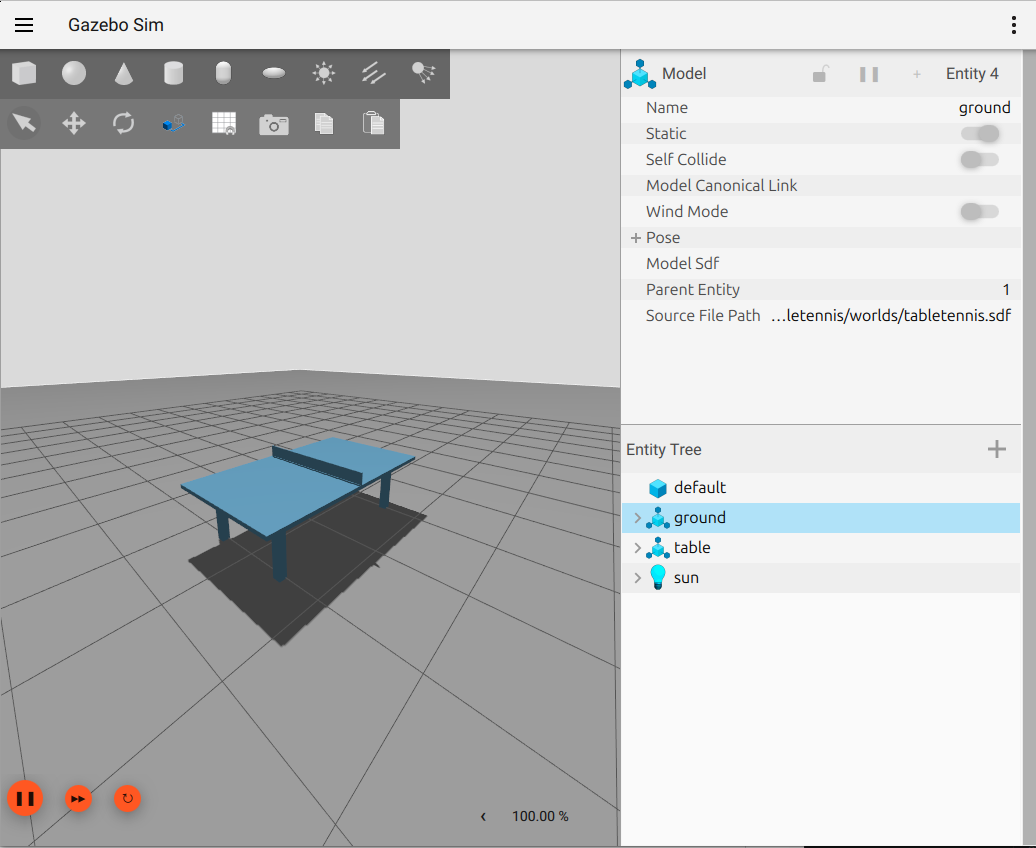
\includegraphics[width=0.85\textwidth]{project_2/tabletennis_plate.png}
  \caption{Die eingebundene Tischtennisplatte in Gazebo: korrekt in Metern
  skaliert (Spielfläche bei $z=0{,}76\,$m) und über Roll\,$+90^\circ$ aufrecht
  gestellt. Sie bildet die Referenzgeometrie und die spätere Zielebene.}
  \label{fig:p2-table}
\end{figure}

\begin{lstlisting}[style=bash,caption={\code{ros2\_ws}-Delta nach Schritt 1 (\# neu / \# angepasst)}]
src/p2_tabletennis/
|- meshes/Tischtennisplatte.stl   # neu (STL aus dem CAD, in mm)
|- worlds/tabletennis.sdf         # neu (Platte als Mesh-Modell + Boden + Licht)
|- launch/table.launch.py         # neu (Gazebo + GZ_SIM_RESOURCE_PATH)
`- setup.py                       # angepasst: data_files (worlds/launch/meshes)
\end{lstlisting}

\subsection{Schritt 2 -- Stereo-Rig und Ball in die Welt integrieren}
Die Wahrnehmung aus Projekt~0.B (Kap.~\ref{ch:projekt0b}) wird übernommen: das
Stereo-Rig und der Ball kommen in \code{tabletennis.sdf}, die Knoten
(\code{ball\_detector}, \code{ball\_tracker}, \code{marker\_viz},
\code{fov\_viz}) werden unverändert aus \code{p0b\_stereo} wiederverwendet.

\paragraph{Welt erweitern.} Stereo-Rig (Blick entlang $+y$ zur Gegnerseite,
Basisbreite $0{,}10\,$m) und der orange Ball (40\,mm, 2{,}7\,g) kommen hinzu.
Damit der Ball \textbf{nicht durch die Platte fällt}, bekommt die Spielfläche
eine \emph{Box-Kollision} (robuster als ein konkaves Mesh) mit Restitution:
\begin{lstlisting}[style=xml,caption={Spielflächen-Kollision + Ball (Auszug aus tabletennis.sdf)}]
<model name="table_top"><static>true</static>
  <pose>0 0 0.74 0 0 0</pose>                 <!-- Oberkante z=0.76 -->
  <link name="link"><collision name="c">
    <geometry><box><size>1.525 2.74 0.04</size></box></geometry>
    <surface>
      <bounce><restitution_coefficient>0.9</restitution_coefficient><threshold>0</threshold></bounce>
      <friction><ode><mu>0.4</mu><mu2>0.4</mu2></ode></friction>
    </surface>
  </collision></link>
</model>

<model name="ball"><pose>0 0.5 1.2 0 0 0</pose>
  <link name="link">
    <inertial><mass>0.0027</mass> ... </inertial>
    <collision name="c"><geometry><sphere><radius>0.02</radius></sphere></geometry>
      <surface><bounce><restitution_coefficient>0.9</restitution_coefficient>
        <threshold>0</threshold></bounce></surface></collision>
    <visual name="v"> ... orange ... </visual>
  </link>
</model>
\end{lstlisting}
\begin{infobox}[title={Aufprall: kein Durchfallen, fast elastischer Stoß}]
Eine \emph{Box}-Kollision der Spielfläche (statt des konkaven Tisch-Meshes)
verhindert Tunneling; mit dem kleinen Zeitschritt ($1\,$ms) bleibt der Ball
sicher auf dem Tisch (Test: Start $z=1{,}2$, nach Sekunden noch springend bei
$z\approx0{,}83$ -- nicht durchgefallen). Der \code{restitution\_coefficient}
$0{,}9$ entspricht dem realen Ball (nahezu elastisch, vgl.\ 26.2.1.4); Reibung
beim Aufprall ist ohne Spin vernachlässigbar.
\end{infobox}

\paragraph{Netz: Box-Kollision statt eigenem STL.} Das Tisch-Mesh enthält das
Netz nur \emph{visuell} -- ohne Kollision fliegt der Ball hindurch. Ein eigener
STL-Körper fürs Netz ist dafür \emph{nicht} nötig (und als dünner, konkaver
Collider sogar tunneling-anfällig); robuster ist -- wie bei der Spielfläche --
eine dünne \emph{Box}-Kollision am Netzort ($y=0$, Höhe $15{,}25\,$cm über der
Platte):
\begin{lstlisting}[style=xml,caption={Netz-Kollision (Auszug aus tabletennis.sdf)}]
<model name="net"><static>true</static>
  <pose>0 0 0.83625 0 0 0</pose>            <!-- 0.76 + 0.1525/2 -->
  <link name="link"><collision name="c">
    <geometry><box><size>1.525 0.01 0.1525</size></box></geometry>
    <surface>
      <bounce><restitution_coefficient>0.1</restitution_coefficient><threshold>0</threshold></bounce>
      <friction><ode><mu>0.8</mu><mu2>0.8</mu2></ode></friction>
    </surface>
  </collision></link>
</model>
\end{lstlisting}
\noindent Die \textbf{niedrige Restitution} ($0{,}1$) und \textbf{hohe Reibung}
nähern das weiche, energiezehrende Verhalten des Netzes an: der Ball prallt nicht
wie von einer Wand ab, sondern verliert Energie und fällt. Eine genauere
\emph{Netzphysik} (nachgiebiges Gewebe) bräuchte ein Soft-Body- bzw.\
Feder-Masse-Netz -- in Gazebo aufwändig; für die Spiel-Logik genügt meist ein
\emph{Netztreffer-Flag} (Let/Fehler) zusätzlich zur Fehlschuss-Erkennung
(26.2.1.5).

\paragraph{Sichtkegel.} Wie in Projekt~0.B (Kap.~\ref{ch:projekt0b},
Sichtfeld-Visualisierung) zeichnet \code{fov\_viz} die Sichtkegel beider Kameras
als \code{MarkerArray} auf \code{/stereo/fov\_markers}; ihr Überlappungsbereich
ist die Zone, in der trianguliert werden kann.

\paragraph{Pipeline per Launch.} Eine Launch-Datei bündelt -- mit allen Lehren
aus 0.A/0.B -- Gazebo, \code{/clock}-Brücke, Bildbrücke, statische Kamera-TF und
die vier Knoten, alle mit \code{use\_sim\_time}:
\begin{lstlisting}[style=py,caption={\code{launch/tabletennis.launch.py} (gekürzt)}]
detector = Node(package='p0b_stereo', executable='ball_detector', parameters=[SIM])
tracker  = Node(package='p0b_stereo', executable='ball_tracker',  parameters=[SIM])
viz      = Node(package='p0b_stereo', executable='marker_viz',    parameters=[SIM])
fov      = Node(package='p0b_stereo', executable='fov_viz',       parameters=[SIM])
static_tf = Node(package='tf2_ros', executable='static_transform_publisher',
    arguments=['--x','0','--y','-1.9','--z','1.1','--roll','-1.5708',
               '--frame-id','world','--child-frame-id','stereo_left_optical'])
return LaunchDescription([resource, gz, clock_bridge, image_bridge,
                          static_tf, detector, tracker, viz, fov, rviz])
\end{lstlisting}
\begin{infobox}[title={Checkliste 0.A/0.B -- in dieser Launch beachtet}]
\code{/clock} gebrückt \emph{und} \code{use\_sim\_time:=true} auf allen Knoten
(sonst ``No transform''); statische TF \code{world}$\rightarrow$%
\code{stereo\_left\_optical}, damit der Kamerarahmen existiert; \code{ogre2}/EGL
fürs Kamerarendering; \code{ApproximateTimeSynchronizer} für L/R-Bilder; Ball
orange ($\Rightarrow$ HSV-Bereich aus 0.B passt); \code{package://} über
\code{GZ\_SIM\_RESOURCE\_PATH}.
\end{infobox}

\paragraph{Terminals und Befehle.}
\begin{lstlisting}[style=bash,caption={Terminal 1 -- bauen + alles starten (Gazebo + RViz + Pipeline)}]
cd ~/ros2_ws
colcon build --packages-select p2_tabletennis
source install/setup.bash
ros2 launch p2_tabletennis tabletennis.launch.py
\end{lstlisting}
\begin{lstlisting}[style=bash,caption={Terminal 2 -- Ballposition anzeigen}]
source ~/ros2_ws/install/setup.bash
ros2 topic echo /ball/point        # gemessene 3D-Position (Triangulation)
ros2 topic echo /ball/estimate     # Kalman-Schaetzung
\end{lstlisting}
\noindent In Gazebo erscheinen Platte, Rig und der (fallende/springende) Ball;
in RViz die Sichtkegel, die Marker (gemessen/geschätzt/Vorhersage) und beide
Kamerabilder. Der \emph{parametrische Gegnerschlag} (Anfangsgeschwindigkeit statt
freier Fall) folgt später; bis dahin lässt sich der Ball in Gazebo mit der Maus
bewegen.
\begin{lstlisting}[style=bash,caption={\code{ros2\_ws}-Delta nach Schritt 2 (\# neu / \# angepasst)}]
src/p2_tabletennis/
|- worlds/tabletennis.sdf       # angepasst: Stereo-Rig + Ball + Box-Kollision (Platte + Netz)
|- launch/tabletennis.launch.py # neu (Welt + Bruecken + Pipeline + RViz)
|- config/tabletennis.rviz      # neu (Marker, FOV, Kamerabilder; Fixed Frame world)
`- package.xml                  # angepasst: exec_depend p0b_stereo u.a.
\end{lstlisting}

\subsection{Schritt 3 -- Balltracking: fliegender Ball}
Damit die Pipeline einen echten Flug verfolgt, muss der Ball über den Tisch
fliegen -- der Gegnerschlag aus 26.2.1.2. Gazebo bietet \emph{keine} API, einem
freien Körper eine Anfangsgeschwindigkeit zu geben (nur \code{set\_pose}). Wir
bewegen den Ball daher \textbf{kinematisch} entlang einer parametrischen
Wurfparabel: der Knoten \code{opponent\_serve} integriert Position und
Geschwindigkeit (mit Tisch-Bounce, vgl.\ 26.2.1.4) und setzt die Ballpose
$\sim$50x/s über den gebrückten \code{SetEntityPose}-Service. Vorteil:
reproduzierbar und mit bekannter Ground Truth -- ideal, um Erkennung und EKF
gegenzuprüfen. (\code{self.p(n)} unten ist Kürzel für
\code{self.get\_parameter(n).value}.)
\begin{lstlisting}[style=py,caption={\code{opponent\_serve} -- Kern (Wurf + Bounce)}]
def start_serve(self):                      # v0 aus speed/azimuth/elevation
    s, sp = self.p('start'), self.p('speed')
    az, el = self.p('azimuth'), self.p('elevation')
    self.pos = [float(s[0]), float(s[1]), float(s[2])]
    self.vel = [sp*cos(el)*cos(az), sp*cos(el)*sin(az), sp*sin(el)]
    self.last_t = None

def tick(self):
    if self.pos is None: return
    now = self.get_clock().now().nanoseconds * 1e-9    # dt aus (Sim-)Zeit!
    if self.last_t is None: self.last_t = now; return
    dt = now - self.last_t; self.last_t = now
    self.vel[2] -= self.p('g') * dt
    for i in range(3): self.pos[i] += self.vel[i] * dt
    if self.pos[2] <= TZ and self.vel[2] < 0 and on_table(self.pos):
        self.pos[2] = TZ; self.vel[2] *= -self.p('restitution')   # Bounce
    self.set_ball(self.pos)                 # SetEntityPose-Service (async)
\end{lstlisting}

\begin{infobox}[title={Lehre: dt aus der Uhr -- und \code{use\_sim\_time} braucht /clock}]
Mit \emph{festem} \code{dt} pro Tick flog der Ball zu schnell, weil der Timer
unter \code{use\_sim\_time} beim Sim-Zeit-Aufholen mehrfach feuert; korrekt ist
\code{dt} aus der \emph{tatsächlichen} Uhr-Differenz. Und: läuft
\code{opponent\_serve} mit \code{use\_sim\_time}, aber \emph{ohne} gebrückte
\code{/clock}, feuert sein Timer nie -- der Ball bleibt stehen (genau der
Checklistenpunkt aus 24.6). Die \code{/clock}-Brücke ist in der Launch deshalb
zwingend.
\end{infobox}

\noindent Den fliegenden Ball verarbeitet die \textbf{unveränderte Pipeline aus
Schritt 2}: \code{ball\_detector} (HSV + sparse Triangulation, 0.B) $\rightarrow$
\code{/ball/point}; \code{ball\_tracker} (Kalman) $\rightarrow$
\code{/ball/estimate} und \code{/ball/prediction}; \code{marker\_viz} zeigt alles
in RViz. Verlässt der Ball das gemeinsame Sichtfeld, stoppt \code{/ball/point} --
die Marker frieren auf der letzten Position ein (Fehlschuss-Indiz, vgl.\
26.2.1.5).

\begin{infobox}[title={Checkliste 23.5/24.6 -- in Schritt 3 beachtet}]
\code{/clock} + \code{use\_sim\_time} (sonst kein Servetimer); Pose-Felder mit
\code{float(\ldots)} gecastet (NumPy-Skalare in ROS-Feldern); \emph{kein}
Custom-Interface -- Auslösung über \code{std\_srvs/Trigger}; der Callback heißt
\code{on\_serve}, nicht \code{handle} (rclpy-Kollision); HSV-Bereich,
L/R-Synchronisation und Disparität unverändert aus 0.B.
\end{infobox}

\paragraph{Terminals und Befehle.}
\begin{lstlisting}[style=bash,caption={Terminal 1 -- alles starten (Welt + Pipeline + Gegnerschlag + RViz)}]
cd ~/ros2_ws
colcon build --packages-select p2_tabletennis
source install/setup.bash
ros2 launch p2_tabletennis tabletennis.launch.py
\end{lstlisting}
\begin{lstlisting}[style=bash,caption={Terminal 2 -- Messung und Schaetzung mitlesen}]
source ~/ros2_ws/install/setup.bash
ros2 topic echo /ball/point        # gemessene 3D-Position (Triangulation)
ros2 topic echo /ball/estimate     # Kalman-Schaetzung
\end{lstlisting}
\begin{lstlisting}[style=bash,caption={Terminal 3 (optional) -- Schlag manuell ausloesen}]
source ~/ros2_ws/install/setup.bash
ros2 service call /opponent/serve std_srvs/srv/Trigger "{}"
\end{lstlisting}
\noindent \code{opponent\_serve} schlägt standardmäßig alle $5\,$s automatisch
auf (Parameter \code{auto\_period}); \code{speed}, \code{azimuth},
\code{elevation} und \code{start} lassen sich anpassen, damit der Ball auf der
Roboterhälfte aufkommt und im Sichtfeld bleibt.
\begin{lstlisting}[style=bash,caption={\code{ros2\_ws}-Delta nach Schritt 3 (\# neu / \# angepasst)}]
src/p2_tabletennis/
|- p2_tabletennis/opponent_serve.py  # neu (parametrischer Gegnerschlag)
|- config/set_pose_bridge.yaml       # neu (Service-Bruecke set_pose)
|- launch/tabletennis.launch.py      # angepasst: set_pose-Bruecke + opponent_serve
|- setup.py                          # angepasst: entry_point opponent_serve
`- package.xml                       # angepasst: ros_gz_interfaces, std_srvs ...
\end{lstlisting}

\subsection{Schritt 4 -- Flugschätzung mit EKF und Luftwiderstand}
Der lineare 0.B-Tracker wird durch ein \textbf{EKF} ersetzt
(\code{flight\_ekf}), das den nichtlinearen Flug aus 26.2.1.4/26.2.1.6 schätzt:
Zustand $\mathbf{x}=[\mathbf{r},\mathbf{v}]^\top$ (6D), Prozessmodell
\begin{equation}
\dot{\mathbf r}=\mathbf v,\qquad
\dot{\mathbf v}=\mathbf g-k\,\lVert\mathbf v\rVert\,\mathbf v,\qquad
k=\frac{\rho\,C_D\,A}{2m}\approx0{,}131\,\mathrm{m^{-1}}.
\end{equation}
Wegen des $\lVert\mathbf v\rVert\mathbf v$-Terms ist das nichtlinear -- der EKF
linearisiert pro Schritt mit der Jacobi-Matrix; für den Geschwindigkeitsblock gilt
\begin{equation}
\frac{\partial \dot{\mathbf v}}{\partial \mathbf v}
= -k\Big(\lVert\mathbf v\rVert\,I+\frac{\mathbf v\mathbf v^\top}{\lVert\mathbf v\rVert}\Big).
\end{equation}
\begin{lstlisting}[style=py,caption={\code{flight\_ekf} -- EKF-Kern (Position gemessen, H=[I\ 0])}]
def ekf_step(self, z, dt):
    F = self._F(self.x, dt)               # Jacobi der Dynamik
    self.x = self._f(self.x, dt)          # Praediktion (nichtlinear, mit Drag)
    self.P = F @ self.P @ F.T + self.Q
    S = self.P[:3, :3] + self.R           # Korrektur, H = [I 0]
    K = self.P[:, :3] @ np.linalg.inv(S)
    self.x = self.x + K @ (z - self.x[:3])
    self.P = (np.eye(6) - K @ H) @ self.P
\end{lstlisting}

\begin{warnbox}[title={Physik im Welt-Frame -- Messungen per TF transformieren}]
Gravitation, Tischebene ($z=0{,}76$) und Abfangebene leben im \textbf{Welt-Frame},
die Messungen (\code{/ball/point}) kommen aber im \emph{optischen Kameraframe}.
Der EKF transformiert sie daher per TF nach \code{world}
(\code{tf\_buffer.transform(msg, 'world')}) und rechnet/publiziert in \code{world}.
In 0.B war das egal (konstante Geschwindigkeit, kein Schwerefeld) -- hier ist es
zwingend.
\end{warnbox}

\paragraph{Auftreffpunkt vorhersagen.} Nach jedem Update wird der Zustand
\emph{ohne} Messung vorwärts integriert (mit Tisch-Bounce) bis zur Abfangebene
$y=y_R$; das ergibt Abfangpunkt und -zeit. Netztreffer und Aus werden dabei wie
in 26.2.1.5 erkannt.
\begin{lstlisting}[style=py,caption={\code{predict\_impact} -- Bounce, Netz, Abfangebene}]
def predict_impact(self):
    x = self.x.copy(); pts = [x[:3].copy()]
    for _ in range(STEPS):
        yprev = x[1]; x = self._f(x, dt)
        if x[2] <= TZ and x[5] < 0 and on_table(x):   # Tisch-Bounce
            x[2] = TZ; x[5] *= -E
        if yprev > 0 >= x[1] and x[2] < NET_TOP:       # Netztreffer -> ungueltig
            return pts, None
        if x[1] <= yR:                                 # Abfangebene erreicht
            return pts, x[:3].copy()
    return pts, None
\end{lstlisting}
\noindent Veröffentlicht werden \code{/ball/estimate} und \code{/ball/prediction}
(wie 0.B, sodass \code{marker\_viz} weiterläuft) sowie \code{/ball/intercept} und
ein Marker (\code{/ball/intercept\_marker}, gelber Zylinder in RViz).

\paragraph{Einfrieren an der Tischmitte (Umsetzung).} Gemäß 26.2.1.4 korrigiert
der EKF nur bis zur Mitte ($y=0$); danach steht die Schätzung fest und es wird
\emph{nicht weitergerechnet} (Performance, ruhige Endanfahrt). Ein neuer Schlag
setzt zurück:
\begin{lstlisting}[style=py,caption={\code{flight\_ekf} -- Einfrieren und Reset}]
def on_point(self, msg):
    z = self._to_world(msg)                  # TF: optical -> world
    if self.frozen:                          # Schaetzung steht fest
        if z[1] > self.reset_y: self._reset()   # nur neuer Schlag setzt zurueck
        else: return                         # sonst: kein EKF-Rechnen mehr
    ...                                      # init / ekf_step / publish
    if self.x[1] <= self.freeze_y:           # Tischmitte erreicht
        self.frozen = True                   # -> Abfangpunkt unveraenderbar
\end{lstlisting}
\noindent Verifiziert: das Einfrieren erfolgt bei $y\approx0$; danach bleiben
Schätzung und Abfangpunkt identisch (keine weiteren Updates), ein Ball wieder bei
$y>1{,}0$ löst den Reset aus.

\begin{infobox}[title={Zwei EKF-Stolpersteine, die wir live trafen}]
\textbf{(1) Geschwindigkeit initialisieren:} mit Startgeschwindigkeit $0$ braucht
der EKF zu lange -- wir setzen $\mathbf v$ aus der \emph{Differenz der ersten
zwei Messungen} ($\mathbf v=(\mathbf z_1-\mathbf z_0)/\Delta t$). \textbf{(2) $Q$
strukturieren:} ein großes $Q$ auf \emph{allen} Zuständen macht die Schätzung
verrauscht; klein auf der Position (das Modell $\mathbf r\!+\!\mathbf v\,\Delta t$
ist exakt), moderat auf der Geschwindigkeit. Damit liegt die \emph{frühe}
Abfangpunkt-Vorhersage (nach $\sim$16 Messungen) bei wenigen bis $\sim$20\,cm und
verfeinert sich mit jeder weiteren Messung (frühe Reaktion, vgl.\ 26.1.8).
\end{infobox}

\begin{infobox}[title={Checkliste 23.5/24.6 -- in Schritt 4 beachtet}]
Mess-Frame korrekt behandelt (TF optical$\rightarrow$\code{world});
\code{use\_sim\_time} + \code{/clock}; Pose-/Punktfelder mit \code{float(\ldots)}
gecastet; \emph{kein} Custom-Interface (\code{PointStamped}, \code{nav\_msgs/Path},
\code{Marker}); Methoden neutral benannt (\code{ekf\_step}, nicht \code{handle}).
Zur Konsistenz nutzt auch \code{opponent\_serve} jetzt Luftwiderstand (gleiche
$k$), und die Schlagparameter sind so gewählt, dass der Ball \emph{über} das Netz
kommt.
\end{infobox}

\paragraph{Terminals und Befehle.}
\begin{lstlisting}[style=bash,caption={Terminal 1 -- alles starten (jetzt mit flight\_ekf)}]
cd ~/ros2_ws
colcon build --packages-select p2_tabletennis
source install/setup.bash
ros2 launch p2_tabletennis tabletennis.launch.py
\end{lstlisting}
\begin{lstlisting}[style=bash,caption={Terminal 2 -- Schaetzung und Abfangpunkt mitlesen}]
source ~/ros2_ws/install/setup.bash
ros2 topic echo /ball/estimate     # EKF-Schaetzung (im world-Frame)
ros2 topic echo /ball/intercept    # vorhergesagter Abfangpunkt
\end{lstlisting}
\noindent In RViz zeigt der gelbe Zylinder den vorhergesagten Abfangpunkt, die
blaue Linie die prädizierte (gebouncte) Bahn. Geht der Schlag ins Netz oder ins
Aus, verschwindet der Abfang-Marker (ungültig).
\begin{lstlisting}[style=bash,caption={\code{ros2\_ws}-Delta nach Schritt 4 (\# neu / \# angepasst)}]
src/p2_tabletennis/
|- p2_tabletennis/flight_ekf.py      # neu (EKF + Luftwiderstand + Auftreffpunkt)
|- p2_tabletennis/opponent_serve.py  # angepasst: Luftwiderstand + Schlag ueber Netz
|- launch/tabletennis.launch.py      # angepasst: flight_ekf statt 0.B-ball_tracker
|- config/tabletennis.rviz           # angepasst: Marker /ball/intercept_marker
`- setup.py / package.xml            # angepasst: flight_ekf, tf2_*-Abhaengigkeiten
\end{lstlisting}

\subsection{Schritt 5 -- Aufschlagregeln, Fehlschuss und Begrenzungswand}
Schritt~5 setzt die Tischtennis-Regeln aus 26.2.1.5 um und macht das Ergebnis
\emph{sichtbar}. Ein neuer Knoten \code{match\_referee} (Schiedsrichter) erkennt
die Aufpraller des Balls, prüft sie gegen die Aufschlag- bzw.\ Ballwechselregeln
und steuert die Visualisierung. Zusätzlich erhält \code{opponent\_serve} einen
echten \textbf{Aufschlag}-Modus -- denn die bisherigen Würfe waren Ballwechsel,
keine Aufschläge.

\paragraph{Regelkonformer Aufschlag im Gegnerknoten.} Der Roboter schlägt nie
selbst auf; der Aufschlag kommt immer vom Spieler. \code{opponent\_serve} kennt
daher zwei Modi (Services \code{/opponent/serve} und \code{/opponent/rally}) und
meldet jeden Schlag auf \code{/opponent/event}, womit der Schiedsrichter seine
Zustandsmaschine zurücksetzt. Die Aufschlagparameter sind so gewählt (offline
geprüft), dass der Ball zuerst auf der eigenen Seite ($y\approx+0{,}5$), dann über
das Netz ($z\approx0{,}97>0{,}9125$) auf die Roboterseite ($y\approx-0{,}5$) springt.
\begin{lstlisting}[style=py,caption={\code{opponent\_serve} -- Modus wählen und Schiedsrichter informieren}]
def _launch(self, mode):
    if mode == 'serve':   # 1. Aufprall eigene Seite, dann ueber Netz
        s, speed, az, el = self.serve_start, 3.0, -1.5708, 0.0873
    else:                 # Ballwechsel: direkt ueber Netz auf Roboterseite
        s, speed, az, el = self.start, 4.5, -1.5708, 0.10
    self.pos = [float(s[0]), float(s[1]), float(s[2])]
    self.vel = [speed*cos(el)*cos(az), speed*cos(el)*sin(az), speed*sin(el)]
    self.event_pub.publish(String(data=mode))   # Schiedsrichter zuruecksetzen
\end{lstlisting}

\paragraph{Aufprall-Erkennung aus den Messungen.} Der Schiedsrichter darf
\emph{nicht} die EKF-Schätzung verwenden -- die ist ab der Tischmitte eingefroren
(Schritt~4) und sähe den Aufprall auf der Roboterseite gar nicht. Stattdessen
transformiert er die Messungen \code{/ball/point} per TF nach \code{world} und
erkennt einen Aufprall als \emph{lokales $z$-Minimum} nahe der Tischhöhe (Vorzeichen
von $v_z$ kippt von $-$ nach $+$), innerhalb der Platte:
\begin{lstlisting}[style=py,caption={\code{match\_referee} -- Aufprall = $z$-Minimum auf Tischhöhe}]
def _check_bounce(self):
    (p0,t0),(p1,t1),(p2,t2) = self.buf          # letzte drei Messungen
    vz_old = (p1[2]-p0[2])/(t1-t0); vz_new = (p2[2]-p1[2])/(t2-t1)
    if not (vz_old < -0.2 and vz_new > 0.2):     return  # kein Umkehrpunkt
    if p1[2] > self.tz + 0.10:                   return  # nicht auf Tischhoehe
    if abs(p1[0]) > self.hw or abs(p1[1]) > self.hl:  return  # ausserhalb Platte
    if t1 - self.last_bounce_t < 0.15:           return  # Entprellung
    self.last_bounce_t = t1
    self._on_bounce('player' if p1[1] > 0 else 'robot')
\end{lstlisting}

\paragraph{Regel-Zustandsmaschine.} Aus der Reihenfolge der Aufprall-Seiten ergibt
sich der Verdikt. Ein Netztreffer (Bahn schneidet $y=0$ unter $0{,}9125\,$m) wird
zusätzlich beim Überqueren der Netzebene erkannt.
\begin{lstlisting}[style=py,caption={\code{match\_referee} -- Aufschlag-/Ballwechselregeln}]
def _on_bounce(self, side):
    self.bounces.append(side); n = len(self.bounces)
    if self.phase == 'SERVE':
        if n == 1 and side == 'robot':  self._fault('nicht auf Aufschlagseite')
        elif n == 2 and side == 'robot': self._valid_serve()  # -> Phase RALLY
        elif n == 2:                    self._fault('2x eigene Seite')
    else:  # RALLY
        if n == 1 and side == 'robot':  self._status('gueltiger Aufprall')
        elif n == 1:                    self._fault('falsche Seite')
        else:                           self._fault('Doppelaufprall')
\end{lstlisting}

\paragraph{Begrenzungswand und Auftreffpunkt in Gazebo.} Die Wand ist als
\emph{durchsichtiges, kollisionsfreies} Box-Visual am Plattenrand ($y=-1{,}30$,
der Abfangebene) in die Welt eingebaut -- der Ball fliegt hindurch. Da Gazebo zur
Laufzeit kein bequemes Umfärben über ROS erlaubt, nutzt der Schiedsrichter einen
Trick \emph{ohne} Materialeingriff: Es gibt \emph{zwei} Wände -- eine grüne
(\code{wall\_ok}) und eine rote (\code{wall\_fault}, sonst unter dem Boden
geparkt). Bei einem Fehlschuss werden sie über dieselbe \code{set\_pose}-Brücke
wie der Ball (Schritt~3) getauscht; ein neuer Ballwechsel tauscht zurück. Der vom
EKF geschätzte Auftreffpunkt (\code{/ball/intercept}) wird als flache Scheibe live
auf die Wand gesetzt.
\begin{lstlisting}[style=py,caption={\code{match\_referee} -- Wand umfärben \& Auftreffpunkt setzen (set\_pose)}]
def _set_wall(self, fault):                      # Tausch statt Umfaerben
    self._move('wall_ok',    0, self.wall_y, self.park_z if fault else self.wall_z)
    self._move('wall_fault', 0, self.wall_y, self.wall_z if fault else self.park_z)

def on_intercept(self, msg):                     # EKF-Schaetzung auf die Wand
    if self.fault: return
    self._move('impact_marker', msg.point.x, self.wall_y, msg.point.z,
               qx=0.7071, qw=0.7071)             # roll 90: Scheibe liegt flach
\end{lstlisting}

\begin{warnbox}[title={Schiedsrichter liest Messungen, nicht die EKF-Schätzung}]
Die Aufprall-Erkennung läuft auf \code{/ball/point} (per TF nach \code{world}),
\emph{nicht} auf \code{/ball/estimate}. Grund: Der EKF friert seine Schätzung an
der Tischmitte ein (Schritt~4) und liefert für die Roboterseite -- wo der
entscheidende zweite Aufprall liegt -- gar keine Updates mehr. Die rohe Messung
sieht die ganze Bahn.
\end{warnbox}

\begin{infobox}[title={Checkliste 23.5/24.6 -- in Schritt 5 beachtet}]
Mess-Frame korrekt (TF optical$\rightarrow$\code{world}); \code{use\_sim\_time} +
\code{/clock} an allen Knoten; \code{set\_pose} wird erst nach
\code{service\_is\_ready()} aufgerufen (kein Blockieren); Pose-Felder mit
\code{float(\ldots)} gecastet; \emph{keine} Custom-Interfaces (\code{PointStamped},
\code{std\_msgs/String}, \code{ros\_gz\_interfaces/SetEntityPose}); Knoten und
Methoden neutral benannt (\code{match\_referee}, \code{process\_world\_point}).
Die Wand ist \emph{ohne Kollision} modelliert -- sonst würde der Ball an ihr
abprallen statt hindurchzufliegen.
\end{infobox}

\paragraph{Terminals und Befehle.}
\begin{lstlisting}[style=bash,caption={Terminal 1 -- alles starten (jetzt mit Schiedsrichter + Wand)}]
cd ~/ros2_ws
colcon build --packages-select p2_tabletennis
source install/setup.bash
ros2 launch p2_tabletennis tabletennis.launch.py
\end{lstlisting}
\begin{lstlisting}[style=bash,caption={Terminal 2 -- Aufschlag/Ballwechsel auslösen, Verdikt mitlesen}]
source ~/ros2_ws/install/setup.bash
ros2 service call /opponent/serve std_srvs/srv/Trigger   # regelkonformer Aufschlag
ros2 service call /opponent/rally std_srvs/srv/Trigger   # Ballwechsel-Schlag
ros2 topic echo /match/status                            # bereit / gueltig / FEHLSCHUSS
\end{lstlisting}
\noindent In Gazebo zeigt die Scheibe auf der durchsichtigen Wand den
EKF-Auftreffpunkt; der reale Ball durchbricht die Wand daneben -- die Differenz ist
die Modellgüte. Bei einem ungültigen Aufschlag (z.\,B.\ \code{/opponent/serve} mit
einem Ballwechsel-artigen Wurf, oder ein Ball ins Netz) färbt sich die Wand rot,
beim nächsten Schlag wieder grün.
\begin{lstlisting}[style=bash,caption={\code{ros2\_ws}-Delta nach Schritt 5 (\# neu / \# angepasst)}]
src/p2_tabletennis/
|- p2_tabletennis/match_referee.py   # neu (Regeln + Fehlschuss + Wand-Visualisierung)
|- p2_tabletennis/opponent_serve.py  # angepasst: Aufschlag-/Ballwechsel-Modus + /opponent/event
|- worlds/tabletennis.sdf            # angepasst: wall_ok/wall_fault + impact_marker (visual-only)
|- launch/tabletennis.launch.py      # angepasst: match_referee gestartet
`- setup.py / package.xml            # angepasst: match_referee, std_msgs
\end{lstlisting}

\noindent Offline verifiziert (Regel-Logik mit synthetischen Bahnen, gleiches
Drag-Modell): gültiger Aufschlag (player$\rightarrow$robot) $\rightarrow$ Wechsel
auf Ballwechsel; erster Aufprall Roboterseite $\rightarrow$ Fehlschuss; zweiter
Aufprall erneut eigene Seite $\rightarrow$ Fehlschuss; Aufschlag ins Netz
$\rightarrow$ Fehlschuss (Netztreffer); gültiger Ballwechsel (ein Aufprall
Roboterseite) $\rightarrow$ kein Fehlschuss.

\subsection{Schritt 6 -- Roboteranbindung}
\emph{[Dokumentation folgt.]} Frühe Abfangbewegung (iterative Verfeinerung),
inverse Kinematik des Portals und Motorsteuerung über den
\code{ros2\_control}-Stack.

% =============================================================
%  ch17_projekt3.tex  --  Projekt 3: Mobiler Roboter
% =============================================================

\chapter{Projekt 3 -- Mobiler Roboter: Odometrie, Navigation, Bewegungserkennung}

\textbf{Ziel:} Mit Stereokamera, Odometrie und Pfadalgorithmen navigieren und
Bewegung erkennen.

\section{ROS\,2-Bausteine}
\begin{longtable}{@{}p{2.6cm}p{12cm}@{}}
\toprule
\textbf{Typ} & \textbf{Konkret} \\
\midrule
Nodes   & \code{stereo\_camera} $\cdot$
          \code{visual\_odometry} oder Radodometrie $\cdot$
          \code{robot\_localization} (EKF: Odom+IMU) $\cdot$
          \code{slam\_toolbox} (Karte) $\cdot$
          \code{nav2} (Planer+Controller) $\cdot$
          \code{motion\_detector} (optischer Fluss/Hintergrundsubtraktion) \\
Topics  & \code{/odom} $\cdot$ \code{/tf} $\cdot$
          \code{/scan} bzw.\ \code{/points2} $\cdot$
          \code{/map} $\cdot$ \code{/cmd\_vel} \\
Actions & \code{nav2\_msgs/NavigateToPose} \\
Parameter & Kostenkarte, Controller-Frequenz, EKF-Konfiguration, Roboterfußabdruck \\
\bottomrule
\end{longtable}

\begin{center}
\begin{tikzpicture}[node distance=5mm and 11mm]
\node[node] (cam) {/stereo\_camera};
\node[node,below=8mm of cam] (vo) {/visual\_odometry};
\node[node,right=14mm of vo] (rl) {/robot\_localization\\\scriptsize (EKF)};
\node[node,right=of rl] (slam) {/slam\_toolbox};
\node[node,right=of slam] (nav) {/nav2};
\node[node,above=8mm of nav] (md) {/motion\_detector};
\draw[flow] (cam) -- (vo);
\draw[flow] (cam) -| (md);
\draw[flow] (vo) -- node[topic,fill=white,inner sep=1pt]{\scriptsize odom} (rl);
\draw[flow] (rl) -- node[topic,fill=white,inner sep=1pt]{\scriptsize tf} (slam);
\draw[flow] (slam) -- node[topic,fill=white,inner sep=1pt]{\scriptsize map} (nav);
\draw[flow] (nav) to[bend right=18]
  node[below,font=\scriptsize]{cmd\_vel} ($(vo)+(0,-1.2)$);
\end{tikzpicture}
\captionof{figure}{Projekt~3: Odometrie $\rightarrow$ EKF-Fusion $\rightarrow$
SLAM $\rightarrow$ Nav2; Bewegungserkennung als paralleler Zweig.}
\end{center}

% =============================================================
%  ch18_projekt4.tex  --  Projekt 4: CAD-Posenerkennung und Greifen
% =============================================================

\chapter{Projekt 4 -- CAD-basierte Posenerkennung und Greifen}

\textbf{Ziel:} Bauteile per Stereokamera über sich matchende CAD-Modelle
erkennen, deren 6D-Lage bestimmen und das Greifen daran anpassen.

\section{ROS\,2-Bausteine}
\begin{longtable}{@{}p{2.6cm}p{12cm}@{}}
\toprule
\textbf{Typ} & \textbf{Konkret} \\
\midrule
Nodes       & \code{stereo\_camera} $\cdot$
              \code{part\_detector} (ORB/SIFT-Matching gegen gerenderte
              CAD-Ansichten \emph{oder} Punktwolke+ICP) $\cdot$
              \code{pose\_estimator} (\code{solvePnP}/ICP $\rightarrow$ 6D-Pose) $\cdot$
              \code{moveit2} (Greifplanung) $\cdot$
              \code{robot\_controller} \\
Topics/Msgs & \code{vision\_msgs/Detection3DArray} $\cdot$
              Pose über \code{/tf} \\
Actions     & MoveIt\,2 \code{MoveGroup} (Planen + Ausführen) \\
Parameter   & CAD-Modellpfade, Matching-Schwellen, ICP-Iterationen,
              Greifvorgaben \\
\bottomrule
\end{longtable}

\begin{center}
\begin{tikzpicture}[node distance=5mm and 12mm]
\node[node] (cam) {/stereo\_camera};
\node[node,right=of cam] (det) {/part\_detector\\\scriptsize CAD-Matching};
\node[node,right=of det] (pe)  {/pose\_estimator\\\scriptsize PnP / ICP};
\node[node,right=of pe]  (mv)  {/moveit2};
\node[node,below=8mm of mv] (rc) {/robot\_controller};
\draw[flow] (cam) -- (det);
\draw[flow] (det) -- (pe);
\draw[flow] (pe)  -- node[topic,fill=white,inner sep=1pt]{\scriptsize 6D pose (tf)} (mv);
\draw[flow] (mv)  -- (rc);
\end{tikzpicture}
\captionof{figure}{Projekt~4: CAD-Matching $\rightarrow$ 6D-Posenschätzung
$\rightarrow$ MoveIt\,2-Greifplanung, angepasst an die erkannte Werkstücklage.}
\end{center}

\section{Zwei Wege zur 6D-Pose}
Für das CAD-Matching gibt es einen klassischen und einen lernbasierten Pfad --
beide enden im selben \code{pose\_estimator} und liefern $(\bm{R},\bm{t})$ über
\code{/tf} an MoveIt\,2:
\begin{enumerate}
\item \textbf{Klassisch (kein Training):} ORB/SIFT-Matching gegen gerenderte
  CAD-Ansichten $\rightarrow$ \code{solvePnPRansac}, \emph{oder} Stereo-Punktwolke
  $+$ ICP gegen die CAD-Punktwolke. Schnell aufzusetzen, aber fragil bei
  texturlosen/glänzenden/symmetrischen Teilen.
\item \textbf{Gelernte Surface Embeddings (SurfEmb-Linie):} das im Theoriekapitel
  beschriebene Zwei-Turm-Netz. Robuster bei genau diesen Industrieteilen, dafür
  Trainingsaufwand. \textbf{Empfehlung:} klassisch starten, lernbasiert
  nachrüsten, wenn die Teile die klassischen Deskriptoren überfordern.
\end{enumerate}
Die theoretischen Grundlagen beider Wege (Rotationsrepräsentationen, kontrastives
Lernen, Two-Tower-Modell, \code{PnP}+\code{RANSAC}, grobe/feine Registrierung,
PointNet++) stehen im Theoriekapitel zur 6-DoF-Posenschätzung.

\section{Inferenz-Pipeline (lernbasiert)}
\begin{enumerate}
\item \textbf{Detektion/Segmentierung} des Objekts im Stereobild $\rightarrow$
  Bildausschnitt (RGB oder RGB-D) plus bekanntes CAD-Modell als Eingang.
\item \textbf{Embedding:} Query-Tower bettet die Pixel ein, Key-Tower die
  CAD-Oberflächenpunkte -- in denselben Merkmalsraum.
\item \textbf{Matching} im Embedding-Raum (nächster Nachbar) $\rightarrow$ dichte
  2D-3D-Korrespondenzen.
\item \textbf{Pose-Hypothesen:} \code{PnP}+\code{RANSAC} sampeln und bewerten
  (Scoring), beste Hypothese wählen.
\item \textbf{Verfeinerung} per ICP $\rightarrow$ finale $(\bm{R},\bm{t})$,
  Modell$\rightarrow$Roboterframe.
\end{enumerate}

\noindent\textbf{Punktwolken-Zusatzschritte} (3D-3D-Pfad): Hintergrund entfernen,
Voxel-Downsampling, statistischer Ausreißerfilter -- vor der Registrierung.

\begin{infobox}[title=Labels sind quasi gratis]
Das CAD-Modell wird in bekannten Posen gerendert $\rightarrow$ Ground-Truth-Pose
\emph{und} die Pixel-Punkt-Korrespondenzen liegen automatisch vor. Kein manuelles
Annotieren, keine Symmetrie-Labels. Das synthetische Training wird per
\textbf{Domain Randomization} und PBR-Rendering (Isaac Sim) gegen den
Sim-to-Real-Gap abgehärtet, optional mit kleinem realem Feintuning-Satz.
\end{infobox}

\section{Stereo als metrische Skala}
Die Stereokamera ist hier nicht nur Bildquelle: Sie löst die
\textbf{Skalenmehrdeutigkeit} der Mono-Ansicht. Tiefe geht entweder als
RGB-D-Zusatzkanal ins Netz oder wird zur Punktwolke rückprojiziert. Erst dadurch
steht $(\bm{R},\bm{t})$ in echten Millimetern -- die Voraussetzung dafür, dass
MoveIt\,2 überhaupt greifen kann. \textbf{Vorsicht:} glänzendes Metall liefert
ungültige Tiefe; saubere Kalibrierung, Rektifizierung und Tiefen-Entrauschung
sind Pflicht.

\section{Bewegte Teile: Pose-Tracking mit Kalman}
Liegt das Teil nicht still (Förderband, armmontierte Kamera), ist die bildweise
Netz-Pose verrauscht und zittrig. Ein \textbf{Kalman-Filter} (vgl.\ Projekt~1/3
und das Kalman-Kapitel) macht aus Einzelschuss ein \emph{Tracking}: Zustand =
Pose (ggf.\ + Geschwindigkeit), Messung = bildweise Netz-Pose;
Prädiktion~$\rightarrow$~Korrektur glättet Jitter, verwirft Ausreißer-Frames und
überbrückt kurze Verdeckungen. Da Rotationen nichtlinear sind: EKF/UKF oder
Filtern auf einer geeigneten Rotationsdarstellung. \emph{Dieselbe
Kalman-Kompetenz wie beim Tischtennisball -- nur auf die 6D-Pose statt die
Ballposition angewandt.}

\section{Hyperparameter und Evaluation}
\begin{longtable}{@{}p{4.4cm}p{9.8cm}@{}}
\toprule
\textbf{Stellgröße} & \textbf{Wirkung} \\
\midrule
Embedding-Dimension & Ausdrucksstärke des Merkmalsraums \\
Kontrastive Temperatur $\tau$ & Schärfe der Zuordnung im Verlust \\
\#Negative / Backbone-Tiefe & Trennschärfe bzw.\ Kapazität \\
LR / Batch / Optimierer & Trainingsdynamik \\
Augmentierungsstärke & Robustheit gegen Sim-to-Real-Gap \\
\code{RANSAC}-Iterationen + Inlier-Schwelle & Ausreißerrobustheit der Posenlösung \\
\#Pose-Hypothesen / Crop-Auflösung & Genauigkeit vs.\ Laufzeit \\
\bottomrule
\end{longtable}
\noindent\textbf{Metriken:} ADD / ADD-S (ADD-S für symmetrische Teile),
geodätischer Rotations- und euklidischer Translationsfehler, RMSE; im
Forschungskontext die BOP-Metriken (VSD, MSSD, MSPD $\rightarrow$ Average Recall)
auf Datensätzen wie T-LESS/ITODD. \textbf{Industrielle KPIs:} Taktzeit/Latenz,
Pick-Erfolgsrate, Falsch-Positiv-Rate -- das sind die Zahlen, die im
Maschinenbeladungs-Einsatz zählen.


% =============================================================
% TEIL VIII  --  Dokumentationsmethodik
% =============================================================
\part{Dokumentationsmethodik}

% =============================================================
%  ch28_dokumentation.tex  --  Dokumentationsmethodik
% =============================================================

\chapter{Vorgehensweise festhalten}

Eine konsistente Dokumentation der Projekte schlägt folgende Struktur und
Werkzeuge vor:
\begin{description}[style=nextline,leftmargin=1.4em]
\item[Versionskontrolle] Alles in \textbf{Git}. Ein Monorepo oder ein Repo je
  Projekt mit klarer \code{README}.
\item[Verzeichnisstruktur]
  \code{/docs} (Theorie, Entscheidungen),
  \code{/design} (CAD, URDF, Frames),
  \code{/hardware} (Stückliste/BOM, Verdrahtung, Pinbelegung),
  \code{/software} (Pakete, Launch-Files, Parameter-YAMLs),
  \code{/calibration} (Kamera-\code{.yaml}),
  \code{/logs} (Tests, \code{ros2 bag}-Aufzeichnungen).
\item[Entscheidungsprotokoll (ADR)] Kurze Notizen ``Warum TMC2209 statt
  A4988?'', ``Warum Jazzy statt Humble?'' -- spart in Monaten viel Grübeln.
\item[Code-Doku] \textbf{Doxygen} (C++) bzw.\ Docstrings + \textbf{Sphinx}
  (Python); \code{rosdoc2} für ROS\,2-Pakete.
\item[Reproduzierbarkeit] Launch-Files und Parameter-YAMLs sind Teil der Doku
  -- sie machen ein Experiment wiederholbar. \code{rqt\_graph}-Screenshots je
  Projekt beilegen.
\item[Nachweise] \code{ros2 bag} zeichnet reale Läufe auf; damit kannst du
  Vision/Kalman \emph{offline} debuggen und Sim vs.\ Real vergleichen.
\end{description}

\begin{infobox}[title=Empfohlene Reihenfolge der Umsetzung]
1.\ Setup (Teil~III)
$\rightarrow$ 2.\ URDF aus CAD + in Gazebo bewegen (Teil~IV)
$\rightarrow$ 3.\ \code{ros2\_control} in Sim, Trajektorie abfahren (Projekt~1 simuliert)
$\rightarrow$ 4.\ Stereokamera real anbinden + kalibrieren (Teil~VI)
$\rightarrow$ 5.\ Kalman/Vision auf simulierten \emph{und} realen Daten
$\rightarrow$ 6.\ Hardware-Interface tauschen, ESP32 + TMC2209 real
$\rightarrow$ 7.\ projektspezifische Logik (Tischtennis, Navigation, Greifen).
Jeder Schritt ist für sich testbar -- das ist der Sinn der
ros2\_control-Trennung.
\end{infobox}


% =============================================================
% Back matter
% =============================================================
\clearpage
\printbibliography[heading=bibintoc,title={Literaturverzeichnis}]

\end{document}
